\documentclass[12pt, oneside]{book}

% UCSD dissertation required geometry
\usepackage[left=1.5in, right=1in, top=1in, bottom=1.25in, centering]{geometry}      
\setlength\parindent{0.5in} \raggedbottom

% Hyperlinks and appendices
\usepackage[hidelinks]{hyperref} \urlstyle{rm}  
\usepackage{appendix}                          

% Math packages
\usepackage{color, amssymb, amsmath, amsthm, verbatim, wasysym, mathrsfs, etaremune}
\usepackage[mathscr]{eucal}

% Formatting and figure packages
\usepackage[font={footnotesize}]{caption}
\usepackage{fancyhdr, lineno, natbib, setspace, indentfirst}
\usepackage{epsfig, float, lscape, scrextend, rotating}

% Custom style sheets for the UCSD dissertation style 
\usepackage{dissertationTableContentTweaks}
\usepackage{dissertationPageStyles}
\usepackage{dissertationRotatedFigures}
\usepackage{dissertationCustomCommands}


% Title page ------------------------------------------------------------------ 
\begin{document}
\pagestyle{title}

\pagenumbering{gobble} \pagenumbering{roman}
\setcounter{page}{1}

\begingroup  
  \centering
  UNIVERSITY OF CALIFORNIA, SAN DIEGO \\[12ex]
  \textbf{On the coupled evolution of oceanic internal waves \\ and quasi-geostrophic flow} \\[12ex]
  A dissertation submitted in partial satisfaction of the requirements for the degree \\
  Doctor of Philosophy \\[6ex]
  in \\[6ex]
  Engineering Sciences (Aerospace Engineering) \\[6ex]
  by \\[6ex]
  Gregory LeClaire Wagner \par
\endgroup

\vfill 
\begingroup
  \noindent
  Committee in charge: \\[2ex]
  \indent Professor William R. Young, Chair \\
  \indent Professor Daniel H.E. Dubin \\
  \indent Professor Sutanu Sarkar \\
  \indent Professor Stefan Llewellyn Smith \\
  \indent Professor Kraig B. Winters \\[6ex]
\endgroup

\begingroup
  \centering
   2016 \par
\endgroup


% Copyright page -------------------------------------------------------------- 
\clearpage
\thispagestyle{empty}
  
\hfill \vfill
\begingroup
  \centering
  Copyright \\ \bigskip
  Gregory LeClaire Wagner, 2016 \\ \bigskip
  Licensed under the Creative Commons Attribution-NonCommercial-NoDerivatives 4.0 International license, \url{http://creativecommons.org/licenses/by-nc-nd/4.0} \par
\endgroup


% Signature page -------------------------------------------------------------- 
\clearpage
\phantomsection \addcontentsline{toc}{chapter}{Signature Page}
\pagestyle{preliminary}
\doublespacing
\hfill \\[6ex]
\begingroup
\noindent The Dissertation of Gregory LeClaire Wagner is approved, and it is acceptable in quality and form for publication on microfilm and electronically: \\[10ex]
\rule{\textwidth}{1pt} \\[8ex]
\rule{\textwidth}{1pt} \\[8ex]
\rule{\textwidth}{1pt} \\[8ex]
\rule{\textwidth}{1pt} \\[8ex] 
\rule{\textwidth}{1pt} \\[-8ex] 
\flushright Chair \\[12ex]
\endgroup

\begingroup
  \centering
  University of California, San Diego \\[2ex]
  2016 \par
\endgroup


% Epigraph -------------------------------------------------------------------- 
\clearpage \phantomsection \addcontentsline{toc}{chapter}{Epigraph}
\singlespacing
\begingroup
	\centering 
	EPIGRAPH \par
\endgroup

$\, $ \vspace{2ex}

\begin{flushright}
Do not be tricked by human-centered views. \\[2ex]
Gary Synder quoting Dogen, \textit{Pearly Everlasting}
\end{flushright}

$\, $ \vfill
 
I had two dreams about him after he died. I don't remember the first one all that well but it was about meetin' him in town somewheres and he give me some money and I think I lost it. But the second one it was like we was both back in older times and I was on horseback goin' through the mountains of a night. Goin' through this pass in the mountains. It was cold and there was snow on the ground and he rode past me and kept on goin'. Never said nothin'. He just rode on past and he had this blanket wrapped around him and he had his head down and and when he rode past I seen he was carryin' fire in a horn the way people used to do and I could see the horn from the light inside of it. About the color of the moon. And in the dream I knew that he was goin' on ahead and that he was fixin' to make a fire somewhere out there in all that dark and all that cold and I knew that whenever I got there he would be there.
And then I woke up.

\begin{flushright}
Cormac McCarthy, \textit{No Country for Old Men}
\end{flushright}


% Table of contents ----------------------------------------------------------- 
\clearpage \phantomsection \addcontentsline{toc}{chapter}{Table of Contents}
\singlespacing
\renewcommand\contentsname{Table of Contents}
{\let\cleardoublepage\relax \tableofcontents}

\clearpage \phantomsection \addcontentsline{toc}{chapter}{List of Figures}
{\let\cleardoublepage\relax \listoffigures}

\clearpage \phantomsection \addcontentsline{toc}{chapter}{List of Tables}
{\let\cleardoublepage\relax \listoftables}


% Acknowledgements ------------------------------------------------------------ 
\clearpage \phantomsection \addcontentsline{toc}{chapter}{Acknowledgements}
\doublespacing
\begingroup
	\centering 
	ACKNOWLEDGEMENTS \medskip \par
\endgroup

Most of the credit and blame for my current state of affairs belongs to my advisor, Bill Young.  Five years and eight months after arriving in San Diego disheveled and somewhat dissatisfied with past adventures in aerospace engineering, I've ended up writing a dissertation on physical oceanography and geophysical fluid dynamics.  How did this happen?  

It is perhaps not too mysterious: one moment in the third week of February at the 2014 Ocean Sciences conference in Honolulu, Bill announced he would ``put me to work'' on near-inertial waves.  And it was Bill who took me in as a wayward third-year engineering student, sent me to the GFD program at Woods Hole in the summer of 2013, told me to take introductory oceanography classes in my fourth year, and guided our daily practice at the blackboard.  These shaped who I am today.

I would not have been advised by Bill if not for an email sent by my first advisor, Eric Lauga.  Eric convinced me against my better judgement to come to San Diego.  He taught me asymptotic methods and his infectious energy kept me afloat in my first three years.  His support after he left for Cambridge --- including a computer, funding, a teaching job, and scientific advice by Skype --- was a PhD's worth.  

Then there is my committee: Kraig, Stefan, Dan, and Sutanu.  Kraig gave invaluable advice on the simulations in \ch \ref{threeComponentModelChapter} and also kept me in line while Stefan hired me to help teach his class and even still endures my complaints about how I never really learned linear theory.  I have had some of my deepest conversations with Rick about how theories of wave-vortex interaction might finally yield progress on two-dimensional turbulence.  Neil guided me in the early stages of my stumbling into the world of geophysical fluid dynamics.  Numerous and varied conversations with Rob, Jerry, David, and Matthew were of no small help.  And I cannot really express my full gratitude for Jen and Amy's invitation to join the ArcticMix cruise in September of 2015.  That experience showed me the power of the dark side and taught me that the ocean is not 2D.  I might have never known.

So many officemates and friends bettered the 2061 days that culminate in this dissertation.  The old Lauga group of Saverio, Gwynn, On Shun, and Art regulated my unruly first-year brain in our exclusive lab-turned-office in EBU II.  Then there were Yi and Roberto and Diego and Fran\c{c}ois, who showed me how many special functions could fit in a single paper and then led me up the South Face of Clyde Minaret.  Lorenzo tolerated every ``buongiorno!'' and used my desk as a printer stand when I started spending most of my time at Scripps.  At Scripps I first shared an office with Ryan, who somehow remained calm when I demanded ``what \textit{is} this Rossby number, anyways?''  Later Cesar taught me that Python is best and shared my frustration with the abuse of spectra and exclaimed ``you've changed!'' when I returned from the Arctic a bit battered by oceanic reality.  The company of science siblings Spencer, Sean, Navid, Nick, Nico, Roy, Ruth, Caitlin, Till, Marion, and many others made procrastination productive, sometimes. 

Part of my education transpired amidst the landscapes of the American West: surfing at Scripps and scrambling at Black's, roaming the rock-studded hills of San Diego's extended backcountry, climbing the silver granite of San Jacinto and the Sierra, skiing but not summiting Cascade volcanos, and exploring the beaches, deserts, forests, and snowpeaks of California and the wildernesses beyond.  Thanks to all who shared them with me.  Thanks to Mr. Fox for leasing me a room within the ponderosa and basalt landscapes of Bend, Oregon, where I wrote most of this dissertation.  Thanks to my brother Andrew for enduring my harshest criticisms and still taking me on rainy ridgeline long runs above Eugene.  And thanks to my parents for their love though my most difficult and headstrong moments and for always being there.

Most of Chapter 2 excepting chapter 2.4 is taken from the paper `Available potential vorticity and wave-averaged quasi-geostrophic flow' published in the Journal of Fluid Mechanics by myself and William R. Young.  This chapter benefited greatly from conversations with Oliver B\"uhler, Jacques Vanneste, and Jin-Han Xie.  

The majority of Chapter 3 excepting chapters 3.B and 3.C is a reprint of the draft `A three-component model for the coupled evolution of near-inertial waves, quasi-geostrophic flow, and the near-inertial second harmonic' submitted to the Journal of Fluid Mechanics by myself and William R. Young.  Chapter 3 was improved by helpful discussions with Cesar Rocha, Nico Grisouard, Kraig Winters, Oliver B\"uhler, Jacques Vanneste and Jin-Han Xie, and by Nico Grisouard's help setting up his customized version of Winters' flowsolve code.  

Chapter 4 would not be nearly as complete if not for the able mathematical assistance of Gwen\"ael Ferrando. 

For the first three years of graduate school I was fortunate to be fully funded by a Focht-Powell fellowship awarded by the Department of Mechanical and Aerospace Engineering at UCSD.  In later years I was partially funded by the National Science Foundation under OCE-1357047. 


% Vita ------------------------------------------------------------------------ 
\clearpage \phantomsection \addcontentsline{toc}{chapter}{Vita}
\singlespacing
\begingroup
	\centering 
	VITA \medskip \par
\endgroup

\begin{table}[htp!]
\begin{tabular}{p{12ex} p{72ex}} 
2009 & Bachelor of Science in Engineering (\textit{Magna Cum Laude}) \\ 
& Aerospace Engineering, University of Michigan, Ann Arbor \\[2ex]
2010 & Master of Science in Engineering \\
& Aerospace Engineering, University of Michigan, Ann Arbor \\[2ex]
2010--2013 & Focht-Powell Fellow, Department of Mechanical and Aerospace Engineering, University of California, San Diego \\[2ex]
2016 & Doctor of Philosophy \\
& Engineering Sciences (Aerospace Engineering) \\
& University of California, San Diego
\end{tabular}
\end{table}

\bigskip

\begingroup
	\centering 
	PUBLICATIONS \bigskip \par
\endgroup

\noindent \textbf{Slow evolution of internal tides in quasi-geostrophic flow} \\
Gregory L. Wagner, Gwen\"ael Ferrando, and William R. Young \\
Journal of Fluid Mechanics, {\it in preparation} \\

\noindent \textbf{A three-component model for the coupled evolution of near-inertial waves, quasi-geostrophic flow, and the near-inertial second harmonic} \\
Gregory L. Wagner and William R. Young \\
Journal of Fluid Mechanics, {\it in review} \\

\noindent \textbf{Available potential vorticity and wave-averaged quasi-geostrophic flow} \\
Gregory L. Wagner and William R. Young \\
Journal of Fluid Mechanics, {\bf 2015}, {\it 785} \\

\noindent \textbf{Mixing by microorganisms in stratified fluids} \\ 
Gregory L. Wagner, William R. Young, and Eric Lauga \\
Journal of Marine Research, {\bf 2014}, {\it 72} \\  

\noindent \textbf{Bubble-Propelled Micromotors for Enhanced Transport of Passive Tracers} \\
Jahir Orozco, Beatriz Jurado-Sanchez, Gregory Wagner, Wei Gao, Rafael Vazquez-Duhalt, 
Sirilak Sattayasamitsathit, Michael Galarnyk, Allan Cortes, David Santillan, Joseph Wang \\
Langmuir, {\bf 2014}, {\it 30}(18) \\

\noindent \textbf{Crawling scallop: Friction-based locomotion with one degree of freedom} \\
Gregory L. Wagner and Eric Lauga \\
Journal of Theoretical Biology, {\bf 2013}, {\it 324} \\

% Abstract -------------------------------------------------------------------- 
\clearpage \phantomsection \addcontentsline{toc}{chapter}{Abstract of the Dissertation}
\label{abstractChapter}

\begingroup  
  \centering  
  
 \mbox{ } \vspace{1.5in}
  
  ABSTRACT OF THE DISSERTATION \\[6ex]
  \textbf{On the coupled evolution of oceanic internal waves \\ and quasi-geostrophic flow} \\[6ex]
  by \\[5ex]
  \doublespacing 
  Gregory LeClaire Wagner \\ 
  Doctor of Philosophy \\
  University of California, San Diego, 2016 \\[4ex]
  Professor William R. Young, Chair \\[4ex]
  
  \endgroup

\doublespacing
Oceanic motion outside thin boundary layers is primarily a mixture of quasi-geostrophic flow and internal waves with either near-inertial frequencies or the frequency of the semidiurnal lunar tide.  This dissertation seeks a deeper understanding of waves and flow through reduced models that isolate their nonlinear and coupled evolution from the Boussinesq equations.  Three physical-space models are developed: an equation that describes quasi-geostrophic evolution in an arbitrary and prescribed field of hydrostatic internal waves; a three-component model that couples quasi-geostrophic flow to both near-inertial waves and the near-inertial second harmonic; and a model for the slow evolution of hydrostatic internal tides in quasi-geostrophic flow of near-arbitrary scale.  This slow internal tide equation opens the path to a coupled model for the energetic interaction of quasi-geostrophic flow and oceanic internal tides. 

Four results emerge.  First, the wave-averaged quasi-geostrophic equation reveals that finite-amplitude waves give rise to a mean flow that advects quasi-geostrophic potential vorticity.  Second is the definition of a new material invariant: Available Potential Vorticity, or APV.  APV isolates the part of Ertel potential vorticity available for balanced-flow evolution in Eulerian frames and proves necessary in the separating waves and quasi-geostrophic flow.  The third result, hashed out for near-inertial waves and quasi-geostrophic flow, is that wave-flow interaction leads to energy exchange even under conditions of weak nonlinearity.  For storm-forced oceanic near-inertial waves the interaction often energizes waves at the expense of flow.  We call this extraction of balanced quasi-geostrophic energy `stimulated generation' since it requires externally-forced rather than spontaneously-generated waves.  The fourth result is that quasi-geostrophic flow can encourage or `catalyze' a nonlinear interaction between a near-inertial wave field and its second harmonic that transfers energy to the small near-inertial vertical scales of wave breaking and mixing.  

\let\cleardoublepage\relax\clearpage


% ----------------------------------------------------------------------------- 
% ----------------------------------------------------------------------------- 
% Body
% ----------------------------------------------------------------------------- 
% ----------------------------------------------------------------------------- 

% Chapter 1 ------------------------------------------------------------------- 
\chapter{Introduction}

\thispagestyle{preliminary}
\pagenumbering{arabic}
\setcounter{page}{1}
\label{introChapter}

\noindent How inappropriate to call this planet Earth when it is quite clearly Ocean. \smallskip

\indent ---Arthur C. Clarke \bigskip \bigskip

From a certain perspective in space, the Earth seems ocean entire.\footnote{\url{http://eoimages.gsfc.nasa.gov/images/imagerecords/46000/46209/earth_pacific_lrg.jpg}}  Ocean covers 70.9\% of the Earth's surface despite billions of years of continental accumulation.  In epochs past, there was only ocean \citep{ward2000rare}.

The ocean's part in climate and life on Earth surpasses its size.  More than 90\% of the heat energy added to the Earth system between 1955 and 2010 is stored in the ocean.  This massive amount of energy corresponds to $36^{\circ}$C of atmospheric warming \citep{levitus2012world}.  Whatever the concerns of mankind, the increase in land surface temperature known as `global warming' is a minor correction to the changes recorded in our warming ocean.

The many oceanic roles in climate emerge from its kaleidoscopic patchwork of motion: the froth of white-capping sea and swell, storm-like eddies spinning off the Gulf Stream, and lumbering internal waves tens to hundreds of meters tall.  The ocean's rotating and density-stratified dynamics entangle each piece spanning from the planetary to the planktonic, placing detailed predictions of ocean dynamics far beyond reach of current technology.  A necessary step toward forecasting climate change is thus the development of new models for ocean physics that are efficient and approximate yet still physically-based and reliable. 

This dissertation contributes to that effort by seeking a deeper understanding of part of the patchwork: the interweaving of two oceanic motions called `internal waves' and `quasi-geostrophic flow' with spatial scales of tens to hundreds of kilometers.  The methods of this dissertation are theoretical, consisting mainly of the development of models that isolate the physics of waves and flow and augmented by a small number of analytical and numerical examples.  It is hoped that further analysis of the models developed in this dissertation will prove useful in interpreting both observations and numerical simulations and in developing ever-better models for oceanic circulation and the evolution of Earth's climate.

\pagestyle{main}

\section{Waves and flow}

Outside surface and bottom boundary layers, oceanic motion is mostly a mixture of internal waves and quasi-geostrophic flow. Waves and flow have similar horizontal space-scales of tens to hundreds of kilometers, but widely disparate time-scales ranging from a few minutes for the fastest waves to months or years for the most slowly-evolving flows.  These pithy oceanic facts are evidenced by six estimates of kinetic energy frequency spectra shown in figure \ref{frequencySpectraIntro}.  The estimates are made from hourly, year-long observations of horizontal velocity in the western Pacific made during the WESTPAC experiment between the summers of 1980 and 1981\footnote{\url{http://www.cmrecords.net/quick/pacific/wp/wp.htm}}.  

\begin{figure}[H]
\centering
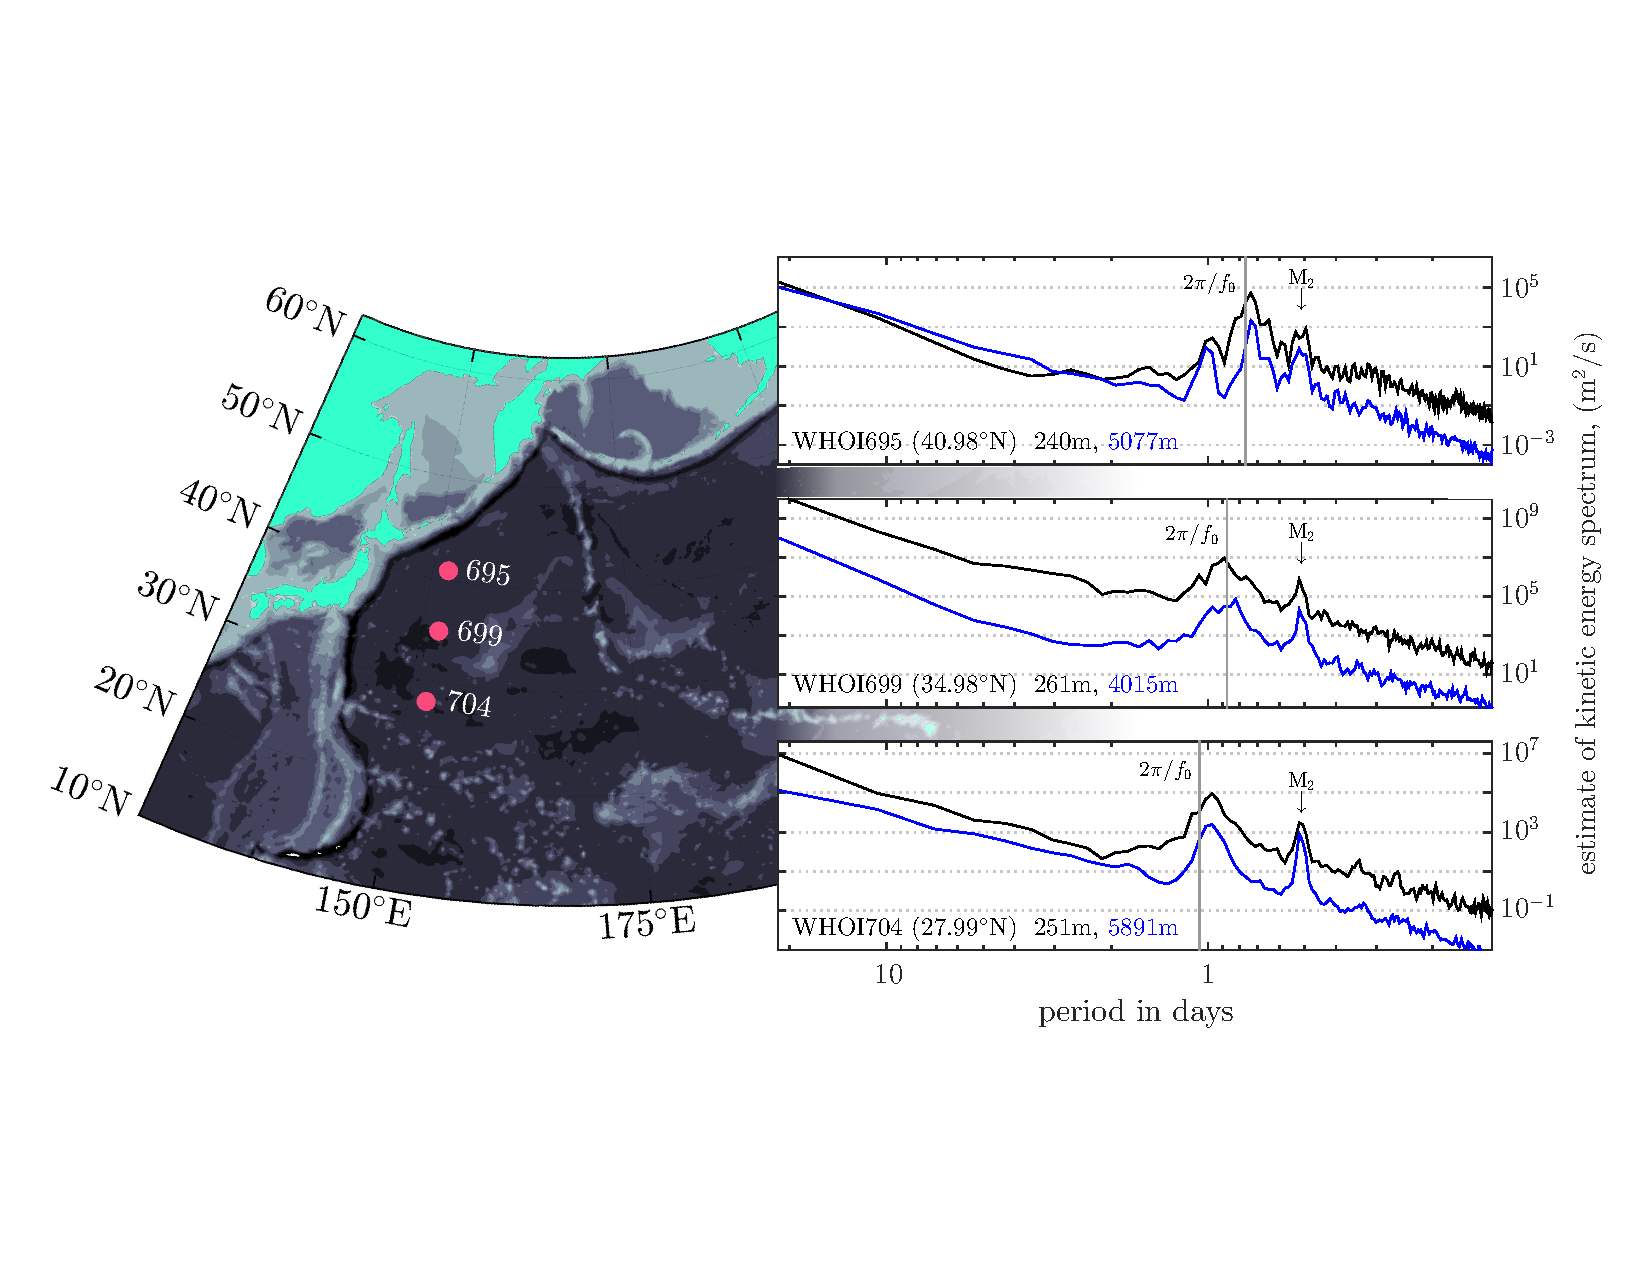
\includegraphics[width = 1\textwidth]{mapAndSpectra}
\caption[Estimates of kinetic energy frequency spectra in three one-year mooring records]{Estimates of kinetic energy frequency spectra in three one-year mooring records from the western Pacific locations shown on the map at left.  At right are kinetic energy spectra from upper-ocean and abyssal instruments on each mooring.  Spectral estimates are the ensemble average of spectra from 35 overlapping and Hamming-windowed 20-day segments extracted from each year-long record.  The arrow and label `$\mathrm{M_2}$' marks the 12.421-hour period of the diurnal tide and a grey line indicates the $2 \pi / f_0 = \left ( 2 \sin \phi \right )^{-1}$-day inertial period at latitude $\phi$.  
Small peaks are discernible at the mixed-harmonic period $2 \pi / (f_0 + \mathrm{M_2}) =  0.31$ and 0.34 days in data from 40.98$^\circ$N and 27.99$^\circ$N, respectively.  
WESTPAC data from OSU's Deep Water Archive$^{2}$ was provided in convenient form by Harper Simmons.}
\label{frequencySpectraIntro}
\end{figure}

Notice first the two conspicuous peaks that appear in every record: one broad and shifting with periods close to one day, and another narrow and fixed at a period of 12.421 hours.  The first peak is the fingerprint of `near-inertial waves' close to the local inertial frequency $f_0 = 4 \pi \sin \phi / \mathrm{day}$ at latitude $\phi$ forced by diverse mechanisms like winds and flow-bathymetry interaction.  The second peak corresponds to a mix of surface tides and internal waves or `internal tides' forced with astronomical precision by the 12.421-hour lunar semidiurnal tide.  A third peak manifests at the solar and lunar diurnal periods close to one day in the record from 40.98$^\circ$N which may correspond to the depth-indepedent surface tide or to the tidally-forced evanescent internal waves explored by \citet{musgrave2016stratified}.  Observe the logarithmic scale: the energy density at inertial and tidal peaks is 100$\times$ greater than at surrounding frequencies.  Their inclination to break and churn the ocean with small-scale turbulence suggests that internal waves make an important contribution to the vertical, diapycnal mixing that sets the ocean's density stratification and draws heat and carbon into the abyss.

\nocite{westpacData}

The inertial and tidal peaks both correspond to relatively high-frequency internal waves.  Moving left from the inertial peak toward lower frequencies and longer periods, kinetic energy density first decreases to a minimum and thereafter increases to what is typically a maximum for each spectrum at the longest observed period.  The sluggish, energy-containing motions associated with this leftward maximum are quasi-geostrophic flows: planetary Rossby waves, meandering currents, and slowly-spinning eddies.  These flows are `quasi-geostrophic' because their leisurely evolution over many inertial periods implies they adhere to a linear geostrophic balance between the inertial Coriolis force and pressure gradient force.  Quasi-geostrophic eddies and currents contain most of the ocean's kinetic energy away from storm-whipped surface layers, and rapidly stir oceanic heat and carbon over decadal time-scales on surfaces of constant density connected to the atmosphere.

In consequence, predicting the Earth system's short-term response to rapid changes in CO$_2$ concentration, for example, requires an approximate description of the quasi-geostrophic stirring not explicitly resolved in coarse resolution models \citep{danabasoglu2012ccsm4,danabasoglu2007effects}.  And efforts for predicting climate evolution over long, hundred-year time-scales requires knowledge of the changing magnitude and spatial distribution of wave-driven diapycnal mixing to accurately describe abyssal absorption of carbon and slow changes in the ocean's density stratification so critical to ocean dynamics.  Approximations of diapycnal mixing may require distinct components to account separately for the mixing driven by internal tides \citep{melet2013sensitivity, green2013comparison,olbers2013global} and near-inertial waves \citep{melet2014sensitivity,jochum2013impact}.  A strong physical basis is necessary for such approximate descriptions of waves and flow to withstand changing atmospheric and oceanic conditions over the course of decades and centuries.

Spurred by the need to better understand internal waves and quasi-geostrophic flow and sustained by a conviction that new mathematical models can yield substantial physical intuition, this dissertation develops models that isolate the nonlinear interaction of oceanic internal waves and quasi-geostrophic flow.  We focus first on evolution of wave-averaged quasi-geostrophic flow in arbitrary and prescribed field of hydrostatic internal waves \ch \ref{APVchapter}.  Next, we develop two models that couple quasi-geostrophic flow to near-inertial waves and their second harmonic in \ch \ref{threeComponentModelChapter} and isolate the slow evolution of internal tides in quasi-geostrophic flow in \ch \ref{internalTideModelChapter}.

\section{Mathematical overtures}

The shape of typical frequency spectra speaks to a dichotomy among energy-containing oceanic motions.  The energy-density minimum or `spectral gap' between the conspicuous high-frequency internal wave peaks and leftward-increasing ramp of low-frequency quasi-geostrophic flow is intrinsic to the ocean's density-stratified and rotating physics: both waves and flow are fundamentally \textit{small-amplitude} motions, or slight perturbations to the ocean's basic state of rapid rotation and strong density stratification.  

The root of this oceanic dichotomy is exposed by a review of the small-amplitude, linear solutions to this dissertation's standard model for oceanic motion, the inviscid, rotating Boussinesq equations on the $\beta$-plane.  The linear solutions to the rotating Boussinesq equations form the basis for the reduced models developed in \ref{APVchapter}, \ref{threeComponentModelChapter}, and \ref{internalTideModelChapter}.  The trek through linear landscapes ends with a glimpse into nonlinear wilds that primes needed mathematical machinery and evokes essential physical ideas.

\subsection{Dynamics of rotating Boussinesq fluids}

The rotating Boussinseq equations are posed in a reference frame that rotates with the Earth at frequency $\Omega = 2 \pi / \text{day}$ and expanded around a static, background density stratification.  Fluid density is decomposed into
\beq
\rho(\bx,t) = \rho_0 + \rho_*(z) + \rho'(\bx,t) \com 
\label{densityDecomposition}
\eeq 
where $t$ is time and $\bx = (x,y,z)$ are Cartesian east, north, and vertical coordinates.  In \eqref{densityDecomposition}, $\rho_0$ is an average or reference density, $\rho_*(z)$ is the background density stratification, and $\rho'$ is the dynamic perturbation associated with fluid motion.  We define the background buoyancy profile $B_*$ and `buoyancy' $b$ associated with the dynamic density perturbation $\rho'$,
\beq
B_*(z) \defn - \frac{g \rho_*(z)}{\rho_0} \qquad \text{and} \qquad b \defn - \frac{g \rho'}{\rho_0} \per
\label{buoyancyDef}
\eeq
The buoyancy $b$ is an acceleration imposed on the fluid by deviations in density from the background profile.  We also decompose pressure into hydrostatic and dynamic components.  The fluid's total pressure field is decomposed into
\beq
-\rho_0 g z + \rho_0 P_{\! *}(z) + \rho_0 p(\bx,t) \com 
\eeq
where $P_{*z} = -g \rho_{*} / \rho_0$ so that $-\rho_0 g z + \rho_0 P_{\! *}$ is the hydrostatic part of pressure and $\rho_0 p$ is the dynamic part of pressure associated with fluid motion.

Two important frequencies intrinsic to density stratification and rotation are the buoyancy frequency, $N$, and inertial or Coriolis frequency, $f$.  The buoyancy frequency is
\beq
N^2 \defn \frac{\dd B_*}{\dd z}  = - \frac{g}{\rho_0} \frac{\dd \rho_*}{\dd z} \per 
\eeq
$N$ is the frequency of gravity- or buoyancy-driven oscillations induced by small \textit{vertical} displacements of fluid.  The inertial frequency is 
\begin{align}
f &\defn 2 \Omega \sin \phi \com \\
&\approx f_0 + \beta y \com \label{betaPlaneApproximation}
\end{align}
where $\phi$ is latitude.  In \eqref{betaPlaneApproximation} we move into a Cartesian reference frame which is tangent to the Earth's surface at the reference latitude $\phi_0$ and make the `$\beta$-plane approximation'.  On the $\beta$-plane, $f$ is expanded around $\phi_0$ so that the local inertial frequency is $f_0 = 2 \Omega \sin \phi_0$ and the latitudinal variation of $f$ is modeled by $\beta y = \left ( 2 \Omega \cos \phi_0 / R \right ) y$, where $R$ is the radius of the Earth.  The local inertial frequency $f_0$ is the frequency of oscillations induced by small \textit{horizontal} displacements of fluid and restored by the displacement's inertial advection of the background rotating velocity field.

The equations used in this dissertation follow from four crucial assumptions: \textit{(i)} the dynamics are inviscid with negligible molecular diffusion and dissipation; \textit{(ii)} density depends linearly on the concentration of one or more scalar quantities; \textit{(iii)} the Boussinesq approximation is valid because density fluctuations are relatively small so that $\rho_*+\rho' \ll \rho_0$; and \textit{(iv)} we can neglect the inertial term $2 \Omega \cos \phi \left ( w \bxh - u \byh \right )$ from the momentum balance because the aspect ratio $H/L$ of considered motions is small so that $w \ll (u,v)$, where $\bu=(u,v,w)$ is the fluid velocity.  Note that we hold off on assuming hydrostatic balance $p=b_z$ in the vertical momentum equation until \ch \ref{APVintro}, despite that disregarding $\left ( 2 \Omega \cos \phi \right ) u$ while assuming $H/L \ll 1$ and $u \gg w$ requires it.  This minor slight-of-hand permits a fuller discussion of linear physics than would be possible under the hydrostatic approximation.  With this caveat, the preceding definitions and assumptions lead to the rotating Boussinesq equations on the $\beta$-plane, 
\begin{align}
\Dt{u} - f v + p_x &=0 \com \label{xmom} \\
\Dt{v}  +f u + p_y &=0 \com \label{ymom} \\
\Dt{w} + p_z &=b \com \label{zmom} \\
\Dt{b} + wN^2&=0 \com \label{buoy} \\
u_x+v_y+w_z &=0 \per \label{cont}
\end{align}
where subscripts with respect to $(x,y,z)$ or $t$ denote partial derivatives, and $\Dt{}$ is the material derivative following the fluid,
\beq
\Dt{} \defn \p_t + \bu \bcdot \bnabla \per
\eeq
In appendix \ref{waveOperatorFormAppendix} we show how \eqref{xmom} through \eqref{cont} can be written in the different and useful `wave operator form'.  The Ertel potential vorticity is 
\begin{align}
\Pi &\defn \bomega_a \bcdot \bnabla \mathcal{B} \com \label{PiDef1} \\
&\defn  \left ( f \bzh + \bomega \right ) \bcdot \left ( N^2 \bzh + \bnabla b \right )\com \label{PiDef2} \\[1ex]
&= f N^2 + N^2 \omega + f b_z + \bomega \bcdot \bnabla b \com \label{PiDef3}
\end{align}
where $\bomega_a$ is absolute vorticity, $\mathcal{B}=B_*+b$ is the total buoyancy field, and $\bomega \defn \bnabla \times \bu$ is relative vorticity with vertical component $\omega = \bzh \bcdot \bomega = v_x - u_y$.   A remarkable property of equations \eqref{xmom} through \eqref{cont} is the material conservation of $\Pi$, so that 
 \beq
\Dt{\Pi} = 0   \per
\label{PVintro}
\eeq
The conservation of $\Pi$ expressed by \eqref{PVintro} is a statement of angular momentum conservation for an effectively constant-density fluid that rotates locally with an effective angular velocity of $\bomega_a/2$ and whose extension along the axes of rotation is tracked by $\bnabla  \mathcal{B}$.  In other words, pulling fluid surfaces apart decreases $\bnabla  \mathcal{B}$ and spins up the fluid by increasing $\bomega_a$.  For the small-amplitude motion of waves and flow, $f N^2$ in \eqref{PiDef3} is by far the largest component of $\Pi$.

\subsection{Lessons of linear dynamics}
\label{linearLessons}

The formulation of \eqref{xmom} through \eqref{cont} means the velocity $\bu$ and buoyancy $b$ are \textit{departures} from a stable basic state in solid body rotation around the $z$-axis with angular velocity $f/2$ and density profile $\rho_0 + \rho_*$.  Waves and flow are both small perturbations to this basic state with small $\bu$ and $b$, which means they are well described by the linear terms in equations \eqref{xmom} through \eqref{cont} obtained by assuming $\Dt{} \approx \p_t$,
\begin{align}
u_t - f_0 v + p_x &= 0 \com \label{xmomLin} \\
v_t + f_0 u + p_y &= 0 \com \label{ymomLin} \\
w_t - b + p_z &= 0 \com \label{zmomLin} \\
b_t + w N^2 &= 0 \com \label{buoyLin} \\
u_x + v_y + w_z &= 0 \label{contLin} \per
\end{align}
Equations \eqref{xmomLin} through \eqref{contLin} are the linearized Boussinesq equations.  Their unsteady solutions are internal waves and their steady solutions are geostrophic flows. 

A conservation law follows by forming $\p_x$\eqref{ymomLin}$- \p_y$\eqref{xmomLin} and using \eqref{contLin} and \eqref{buoyLin}, 
\beq
\p_t \left [ v_x - u_y + \p_z \left ( \frac{f_0 b}{N^2} \right ) \right ] \defn N^2 Q_t = 0 \com
\label{linearAPV}
\eeq
where we recall that $\omega = \bzh \bcdot \bomega = v_x - u_y$ is the vertical component of vorticity.  In equation \eqref{linearAPV} we have defined $Q$, the linear `Available Potential Vorticity', or APV.  Linear APV is synonymous with the standard expression for quasi-geostrophic potential vorticity.  The linearized APV does not evolve in \eqref{xmomLin} through \eqref{contLin}: for internal waves $Q=0$ and for geostrophic flow $Q = Q(\bx)$ is constant in time.  The general definition of nonlinear APV in \ch \ref{APVsec} is one of the main accomplishments of this dissertation.  Notice that \eqref{linearAPV} is not equal to the linear parts of Ertel PV in \eqref{PiDef2}.  Thus internal waves generate non-trivial signatures in $\Pi$ even while $Q=0$.  This point is central to the utility of APV.

\subsubsection{Waves} 

When $f=f_0$ is constant, a short series of manipulations on \eqref{xmomLin} through \eqref{contLin} discussed in detail in appendix \ref{waveOperatorFormAppendix} leads to a single equation for $w$,
\beq
\Big [ \p_t^2 \left ( \hlap + \p_z^2 \right ) + f_0^2 \p_z^2 + N^2 \hlap \Big ] w = 0 \com
\label{waveEqn}
\eeq
where we define the horizontal Laplacian $\hlap \defn \p_x^2 + \p_y^2$.  Equation \eqref{waveEqn} is the internal wave equation.  When $f$ and $N$ are constant and the considered domain is either infinite or a periodic box, we can decompose $w$ into the sinuosoids $w = \exp \left ( \ii \bk \! \bcdot \! \bx - \ii \sigma t \right ) \hat w(\bk,\sigma)$, where $\sigma$ is frequency and $\bk = \left ( k , \ell, m \right )$ is wavenumber.  Then \eqref{waveEqn} implies that $\bk$ and $\sigma$  satisfy the \textit{dispersion relation},
\beq
\sigma^2 = \frac{f_0^2 m^2 + N^2 \left ( k^2 + \ell^2 \right ) }{k^2 + \ell^2 + m^2} \per
\label{dispersionRelation}
\eeq
Equation \eqref{dispersionRelation} shows that the frequency of linear, freely-propagating internal waves always lies between $f_0$ and $N$, whether $f_0 < N$ or $N < f_0$.  When $N$ is not constant but varies slowly compared to $1/m$, equation \eqref{dispersionRelation} becomes a local approximation.  A stationary phase analysis developed by \citet{lighthill2001waves} in chapters 3.7 and 3.8 of his book shows that energy in the linear, Fourier-decomposed wave field travels at the `group velocity' $\mathbf{U} = \bnabla_{\! \! \bk} \hspace{0.1ex} \sigma$ corresponding to the vector $\bx/t$ at which the phase function $\theta = \bk \bcdot \bx / t - \sigma$ is stationary.  This indicates the group velocity of waves near frequency $f_0$ or $N$ is small where $\sigma$ changes slowly with $\bk$.

The dispersion relation in \eqref{dispersionRelation} implies that waves with frequency close to $f_0$ have $(N k / f_0 m)^2 \ll 1$ and thus large horizontal scales and small vertical scales under typical oceanic conditions where $f_0 \ll N$.  These nearly-horizontally-uniform `near-inertial' motions have small horizontal pressure gradients, so that \eqref{xmomLin} and \eqref{ymomLin} combine into 
\beq
\U_t + \ii f_0 \U \approx 0 \com \qquad \text{where} \qquad \U \defn u + \ii v \per
\label{inertialWaves}
\eeq
The solution to \eqref{inertialWaves} is $\U \approx \ee^{-\ii f_0 t} A(\bx,t)$, where $A$ is a near-arbitrary function of space that evolves slowly in the linear equations to reflect slight departures of $\U$ from the inertial frequency.  When $A=A(\bx)$ is stationary this type of motion is often called an `inertial oscillation', though a better name is `pure inertial wave'.  At the other end of the spectrum are motions with small horizontal scales and large vertical scales.  These near-buoyancy waves have small vertical pressure gradients so that \eqref{zmomLin} and \eqref{buoyLin} merge into
\beq
\W_t + \ii N \W \approx 0 \com \qquad \text{where} \qquad \W \defn w + \ii b/N \per
\label{buoyancyWaves}
\eeq
The solution to \eqref{buoyancyWaves} is $\W \approx \ee^{-\ii N t} A(\bx,t)$, where again $A$ is an near-arbitrary function of space and slowly evolves in time.  In the real and  heterogeneous ocean, pure inertial or buoyancy waves cannot exist.  Motions are always \textit{near}-inertial or \textit{near}-buoyancy.  

The fact that $\U$ and $\W$ have arbitrary spatial structure in \eqref{inertialWaves} and \eqref{buoyancyWaves} reflects the important fact that dispersion only weakly constrains the spatial structure of malleable near-inertial and near-buoyancy waves.  The weak dispersion and correspondingly slow propagation of near-inertial and near-buoyancy waves means that oceanic heterogeneities not accounted for in the linear equations, like quasi-geostrophic flow, small-scale turbulence, or surface waves, are important in determining their spatial structure and ultimate evolution.

\subsubsection{Flow} 

The preceding discussion ignores a special and important non-trivial solution to \eqref{waveEqn}: $w=0$.  This solution corresponds to steady solutions to the linear Boussinesq equations, in which case \eqref{xmomLin} through \eqref{zmomLin} reduce to
\begin{align}
f_0 v &= p_x \com \label{vbalance} \\
- f_0 u &= p_y \com \label{ubalance} \\
b &= p_z \per \label{hbalance} 
\end{align}
Equations \eqref{vbalance} and \eqref{ubalance} are the conditions of geostrophic balance and \eqref{hbalance} is the condition of hydrostatic balance.  Geostrophic flow obeys $u_x + v_y = 0$ and can be described by the geostrophic streamfunction
\beq
\psi \defn p / f_0 \com \qquad \text{so that} \qquad (u,v,b) = \left ( - \psi_y , \psi_x , f_0 \psi_z \right ) \per
\eeq
Unlike internal waves, geostrophic flow does not evolve in the linear Boussinesq equations with $f=f_0$.  Its evolution must appeal either to nonlinearity or effects of the Earth's curvature through $\beta$.

\subsubcustom{Limits of linearity.}  In the nonlinear equations in \eqref{xmom} through \eqref{cont}, both waves and flow acquire slow but non-infinite time-scales associated with slight departures from the linear balances in \eqref{xmomLin} through \eqref{contLin}.  If we denote the fast wave time-scale $\tt$ and the flow time-scale $\bar t$, the nearly-linear solutions to \eqref{xmom} through \eqref{cont} become
\beq
Q = Q(\bx,\bar t) \com \qquad \text{and} \qquad w(\bx,\tt,\bar t) = \sum_{n} \ee^{-\ii \sigma_n \tt} A_n(\bx, \bar t) \per
\eeq
The methods of this dissertation are, crudely put, to \textit{(i)} derive an equation for the slow evolution of $Q$ which isolates the `average' effects of waves over the long time-scales of $\bar t$, and \textit{(ii)} restrict attention to one or two frequencies $\sigma_n$ and derive slow evolution equations for $A_n$ that couple to the slow evolution of $Q$.  We next discuss how to isolate the slow evolution of $Q$ from \eqref{xmom} through \eqref{cont} in the classic case of quasi-geostrophic flow.

\subsection{Interaction and non-interaction of waves and flow}
\label{APVintro}

One of the main accomplishments of this dissertation is the definition of a new material invariant named `Available Potential Vorticity', or APV.  A comprehensive introduction to APV is given in \ch \ref{APVsec}.  One definition of APV is 
\beq
Q(\bx,t) \defn \Pi(\bx,t) - \Pi_*(\bx-\bXi) \com
\label{APVdef}
\eeq
where $\Pi$ is Ertel PV defined in \eqref{PiDef3}, $\Pi_* \defn f N^2$ is its static `background' part, and $\bXi(\bx,t)$ is exact nonlinear particle displacement defined through $\Dt{\bXi} = \bu$.  Because $\Dt{\Pi} = 0$ and $\Dt{\left ( \bx - \bXi \right ) } = 0$, APV is materially conserved, so that
\beq
\Dt{Q} = 0 \per
\eeq
APV isolates the part of potential vorticity with a meaningful, intrinsic evolution.  When $f=f_0$ is constant, $Q$ expands for $\omega / f_0 \sim b_z / N^2 \ll 1$ into
\beq
Q = N^2 \left [ \omega + \p_z \left ( \frac{f_0 b}{N^2} \right ) \right ] + \bomega \bcdot \bnabla b - \frac{f_0 \Lambda_{zz}}{N^2} \half b^2 + \cdots \com
\eeq
where $\Lambda \defn \ln N^2$. 

The APV equation opens a relatively straightforward path to the result that the evolution of quasi-geostrophic flow is independent from waves \textit{of equal `magnitude'} to leading-order in Rossby number.  This result was shown by \cite{bartello1995geostrophic} and \cite{majda1998averaging} for the rotating Boussinesq equations and by \cite{warn1986statistical} and \cite{dewar1995fast} for the shallow water equations.   We define two non-dimensional parameters, 
\beq
\ep \defn \frac{U}{f_0 L} \com \qquad \text{and} \qquad \Bu \defn \left ( \frac{N_0 H}{f_0 L} \right )^{\! \! 2} \com
\eeq
where $N_0$, $U$, $H$, and $L$ are characteristic scales for $N$, velocity, height, and horizontal extent of the motion.  The parameter $\ep$, which is both the Rossby number as well as a measure of wave amplitude, is assumed small.  Note that this definition of $\ep$ differs from that in section \ref{linearSec}, where $\ep$ is a measure of wave amplitude only and the Rossby number is $\ep^2$.  The parameter $\Bu$ is the Burger number, which measures the magnitude of the horizontal pressure gradient relative to inertia.  The ratio $f_0 / N_0$ is almost always small in the Earth's ocean except for isolated, abyssal places.  The standard quasi-geostrophic assumption is that $H / L \sim f_0 / N_0 \ll 1$ such that $\Bu = O(1)$.  This assumption reduces the vertical momentum equation \eqref{zmom} to the statement of hydrostatic balance, $p_z = b$.

The bread-and-butter asymptotic method of this dissertation is the multiple-scale `two-time' expansion, which assumes the existence of two time-scales: a fast wave time-scale $\tt \sim f_0^{-1}$, and a slow flow-evolution time-scale $\bar t \sim \left ( \ep f_0 \right )^{-1}$.  Time-derivatives are accordingly split into
\beq
\p_t \mapsto \p_{\tt} + \ep \, \p_{\bar t} \com
\eeq
The non-dimensional APV equation becomes
\beq
Q_{\tt} + \ep \left ( \bu \bcdot \bnabla Q + Q_{\bar t} \right ) = 0 \per
\label{ndAPVIntro}
\eeq
All quantities are expanded in $\ep$, so that APV has the expansion
\beq
Q = \underbrace{\mystrut{2ex} N^2 \left [  \omega_0 + \p_z \left ( \tfrac{b_0}{N^2} \right ) \right ] }_{\defn Q_0} \, + \, \ep \, \Big ( \underbrace{\mystrut{2ex}  \bomega_0 \bcdot \bnabla b_0 + N^2 \left [ \omega_1 + \p_z \left ( \tfrac{b_1}{N^2} \right ) \right ]}_{\defn Q_1} \Big ) + \cdots 
\eeq
Notice that $Q_0$ is just the linear APV from \eqref{linearAPV}.  

The leading-order velocity $\bu_0$ obeys the linear equations \eqref{xmomLin} through \eqref{contLin} with hydrostatic balance $p_{0z} = b_0$ replacing \eqref{zmomLin}.  By averaging over the fast time-scale, $\bu_0$ can be decomposed into waves, $\buu_0$, and flow $\avbu_0$, 
\beq
\bu_0 = \avbu_0 + \buu_0 \per
\eeq
The average is defined so that $\bar{\tilde{a}} = 0$ and $\overline{\left ( a_{\tt} \right )} = 0$, when $a(\bx,\tt, \bar t)$ is any variable decomposed into fast and flow components.  $\buu_0$ is a rapidly oscillating wave field governed approximately by \eqref{waveEqn} and $\avbu_0$ is slowly-evolving quasi-geostrophic flow.  $\avbu_0$ obeys geostrophic and hydrostatic balance and can thus be expressed by a geostrophic streamfunction, 
\beq
\psi \defn \bar p_0 \com \qquad \text{so that} \qquad \left ( \bar u_0, \bar v_0 , \bar b_0 \right ) = \left ( - \psi_y , \psi_x , \psi_z \right) \per
\eeq
The non-interaction result follows in two-steps.  At leading-order, the APV equation amounts to a restatement of \eqref{linearAPV},
\beq
N^{-2} Q_{0 \tt} = \p_{\tt} \left [ \omega_0 + \p_z \left ( \frac{b_0}{N^2} \right )  \right ] = 0 \per
\label{o0APVintro}
\eeq
The integral of \eqref{o0APVintro} implies that $Q_0 = \bar Q_0 (\bx, \tau)$ does not depend on the fast time.  The $O(\ep)$ terms in the APV equation \eqref{ndAPVIntro} are
\beq
Q_{0\bar t} + Q_{1\tt} + \bu_0 \bcdot \bnabla Q_0 = 0 \per
\label{o1APVintro}
\eeq
Because $Q_0$ does not depend on the fast time $\tt$, the time-average of \eqref{o1APVintro} is
\beq
Q_{0\bar t} + \avbu_0 \bcdot \bnabla Q_0 = 0 \per
\label{nonInteraction}
\eeq
Equation \eqref{nonInteraction} is the ordinary quasi-geostrophic equation.  If we restore dimensionality, and define the `quasi-geostrophic potential vorticity' as $q = Q_0 / N^2$, \eqref{nonInteraction} rearranges into the `standard' quasi-geostrophic equation with $\beta=0$, 
\beq
q_{\bar t} + \J \left ( \psi, q \right ) = 0 \com \qquad \text{with} \qquad q \defn \left ( \p_x^2 + \p_y^2 + \p_z \frac{f_0^2}{N^2} \p_z \right ) \psi \per
\label{QGintro}
\eeq
The operator $\J(a,b) = a_x b_y - a_y b_x$ is the Jacobian so that $\p_t + \J(\psi, \cdot) = \p_t +  \avbu_0 \bcdot \bnabla$ is the wave-averaged and leading-order material derivative.  To time-scales at least as long as $\left ( \ep f_0 \right )^{-1}$, the evolution of $q$ is independent from $\buu_0$ and thus internal waves.  On longer time-scales, however, the independence of $q$ and $\buu_0$ is not secure. 

\section{The shape of things to come}

This dissertation develops models in which waves and flow \textit{coevolve} and interact with two-way coupling.  For this purpose we revise the assumption in \ch \ref{APVintro} that both waves and flow are leading-order solutions to \eqref{xmom} through \eqref{cont}.  Instead, we assume that waves are `strong', and flow is `weak', so that $\bu_0 = \buu_0$ and the leading-order solution of \eqref{xmom} through \eqref{cont} is a rapidly oscillating wave field.  In this case, the quasi-geostrophic flow is part of the first-order velocity $\bu_1$, the leading contribution to APV is $Q_1$, the small parameter $\ep$ measures wave steepness, and the Rossby number is $\Ro = \ep^2$.

The work of \ch \ref{APVchapter} is then to find a slow evolution equation for $q = Q_1 /N^2$.  This equation resembles the classical quasi-geostrophic equation in \eqref{QGintro} but for two crucial differences: first, geostrophic balance is modified and obeyed only by the Lagrangian-mean flow, rather than the Eulerian-mean.  The modified balance conditions are given in \eqref{uLdef1} and differ from the traditional balance conditions in \eqref{ubalance} and \eqref{vbalance}.  Second, waves contribute to the APV balance that defines $q$ in \eqref{QGintro}.  In consequence the APV equation in \eqref{eq1} and \eqref{eq2} becomes, with $\beta = 0$,
\beq
q_{\bar t} + \J \left ( \psi , q \right ) = 0 \com \qquad \text{with} \qquad q \defn \left ( \p_x^2 + \p_y^2 + \p_z \frac{f_0^2}{N^2} \p_z \right ) \psi + \qdag \per
\label{newAPVintro}
\eeq
Compare \eqref{newAPVintro} to \eqref{QGintro}.  The new `wave contribution to APV', $\qdag$ in \eqref{newAPVintro}, is defined in \eqref{eq3} and modifies the evolution of quasi-geostrophic flow.  The surprisingly mundane and kinematic origins of $\qdag$ are discussed in \ch \ref{waveAveragedKinematics}.

The contribution of $\qdag$ to $q$ in \eqref{newAPVintro} does \textit{not} imply that `waves have APV'.  The APV in $q$ is still a material invariant advected on the time-averaged particle trajectories described by $\psi$ and decidedly a quantity wholly separate from waves.  Instead, the inclusion of $\qdag$ in the APV balance implies that waves are associated with their own, wave-induced balanced flow that partakes in flow evolution by advecting $q$.  We make this explicit by exploiting the fact that $q$ is linear in $\psi$, which permits the decomposition
\beq
\psi = \psiq + \psiw \com
\label{balancedFlowDecompositionIntro}
\eeq
where $\psiq$ and $\psiw$ are defined through
\beq
q = \left ( \p_x^2 + \p_y^2 + \p_z \frac{f_0^2}{N^2} \p_z \right ) \psiq \com \quad \text{and} \quad - \qdag = \left ( \p_x^2 + \p_y^2 + \p_z \frac{f_0^2}{N^2} \p_z \right ) \psiw \per
\eeq
The balanced flow thus has two parts: an ordinary, APV-associated part in $\psiq$, and a wave-induced part in $\psiw$.  The effect of waves on flow evolution is expressed entirely in the advection of $q$ by $\psiw$.  

The wave-induced balanced flow $\psiw$ is a nonlinear correction that refines linear hydrostatic wave solutions to better satisfy the nonlinear equations in \eqref{xmom} through \eqref{cont}.  Because infinite plane progressive waves are exact solutions to the nonlinear equations \eqref{xmom} through \eqref{cont} when $N$ and $f$ are constant, such waves have $\qdag=0$ and no wave-induced balanced flow.  Even vertically-standing but horizontally infinite waves have no wave-induced flow because $\qdag$ and $\psiw$ are horizontally uniform.  In that case $\psiw$ corresponds to steady $z$-dependent corrections to the pressure and buoyancy fields.  Deeper intuitions on wave-induced balanced flows are developed in \ch \ref{examples}.

Infinite plane waves are mathematical figments that do not exist in the Earth's ocean where wave forcing is time-varying and spatially-modulated, $f$ and $N$ are not constant, and heterogeneities like quasi-geostrophic flow advect, refract, and otherwise distort wave fields aspiring to linearity.  Such distortion enhances wave field nonlinearity, leading to stronger $\psiw$ and wave `feedback' on flow evolution and exposing the incompleteness of equation \eqref{newAPVintro}: the wave property $\qdag$ is not known in general and worse, depends on $\psiq$ and $q$.  To close the APV equation in \eqref{newAPVintro} we need an equation that describes the slow evolution of the wave field and $\psiw$ in quasi-geostrophic flow describe by the distribution of $q$.  This is the goal of chapters \ref{threeComponentModelChapter} and \ref{internalTideModelChapter}, which separately focus on coupling \eqref{newAPVintro} to one of the two conspicuous peaks in figure \ref{frequencySpectraIntro}: the near-inertial peak in \ch \ref{threeComponentModelChapter}, and the tidal peak in \ch \ref{internalTideModelChapter}.  

The derivation of the near-inertial equation in \ch \ref{niwexpansion} is particularly tractable due to the weak dispersion of near-inertial waves.  Motivated by observations and simulations of the Boussinesq equations that persistently observe near-inertial second harmonic waves with frequency $2f_0$ when near-inertial waves interact with quasi-geostrophic flow \citep{DAsaro1995,niwa1999response,danioux2008propagation}, the model is extended to include the nonlinear production and slow evolution of waves frequency $2f_0$.  The result is a closed three-component model that describes the simultaneous evolution of APV, the amplitude of the near-inertial waves, and the amplitude of the near-inertial second harmonic.  Peculiarly, the two distinct adiabatic invariants of the model identified in \ch \ref{conservationlaws} imply that near-inertial waves can extract energy from quasi-geostrophic flows under ordinary oceanic conditions.  Chapter \ref{simulations} compares numerical solutions to the three-component model with the Boussinesq equations and \ch \ref{physicalImplications} discusses the physics these solutions imply.  

The interaction between internal tides and quasi-geostrophic flow is tackled in \ch \ref{internalTideModelChapter}.  Distilling the slow evolution of internal tides is more difficult than the near-inertial case and equivalent to finding a slow evolution equation for general-frequency hydrostatic internal waves in quasi-geostrophic flow.  Key to deriving the internal tide model is the method of reconstitution \citep{roberts1985introduction}, which in a sense generalizes the derivation of the $2f_0$ equation in \ch \ref{threeComponentModelChapter}.  Two solutions to the hydrostatic wave model for barotropic flow are discussed in \ch \ref{examplesTide}.  Further work remains to couple the slow hydrostatic wave evolution to the modified quasi-geostrophic system in \eqref{eq1} through \eqref{eq3}.


% Chapter 2 ------------------------------------------------------------------- 

\let\cleardoublepage\relax\clearpage
\chapter{Available potential vorticity and wave-averaged quasi-geostrophic flow}
\label{APVchapter}
\thispagestyle{preliminary}

\section{Introduction}

The quasi-geostrophic (QG) approximation is a reduced description of the slow dynamics of planetary flows which, being perturbations on a state of rapid rotation and strong stratification, are nearly in geostrophic and hydrostatic balance.  QG is simple and elegant and describes many characteristics of observed flows in the atmosphere and ocean.  A main motivation for the QG approximation is the exclusion of inertia-gravity internal waves, which oscillate on super-inertial frequencies much faster than the sub-inertial time scales of QG flow evolution.  This time-scale separation motivates a central assumption in QG: internal waves have negligible effect on slow, nearly-balanced flow.  

The assumption of weak interaction between internal waves and QG flow was assessed by B\"uhler \& McIntyre (1998, BM hereafter), who used the Generalized Lagrangian Mean (GLM) to demonstrate that average wave terms contribute to the balance of the materially conserved, wave-averaged quasi-geostrophic potential vorticity (QGPV).  This `wave-QG' theory is a significant extension to the QG framework and demands detailed understanding.  With this motivation, we provide an alternative Eulerian derivation of wave-QG which avoids the GLM transformation of the Boussinesq equations.  Our derivation, which relies instead on a multiple time-scale expansion, confirms the main results of BM while extending the validity of wave-QG to non-uniform buoyancy frequency $N(z)$, and thus non-uniform background potential vorticity $f_0 N^2(z)$.  We make no assumption about spatial scale separation between waves and balanced flow,  so that our theory is relevant to mesoscale atmospheric flows and oceanic meso- and submeso-scale flows where motion is mixed between large-scale waves and balanced geostrophic turbulence (Callies, B\"uhler \& Ferrari, 2014). \nocite{callies2014transition}

The challenge of non-uniform background stratification motivates the definition of a new material invariant: available potential vorticity (APV).  APV exactly eliminates the part of Ertel PV that plays only a passive, background role, thereby isolating the part of PV available for flow evolution.  APV proves crucial for the derivation of wave-QG, where strong internal waves generate large but unimportant Eulerian fluctuations in Ertel PV.  The physical significance of APV is suggested by the emergence of QGPV at leading-order in a low-Rossby-number expansion of the exactly conserved APV.
 
Like the standard QG case \citep{Pedlosky,Salmon, Vallis}, the evolution of balanced flow in an internal wave field is described in terms of the quasi-horizontal advection of QGPV, $q$, by a geostrophic streamfunction $\psiL$,
 \beq
q_t +\sJ(\psiL,q)=0 \com
\label{eq1}
\eeq
where $\sJ(\psiL,q) = \psiL_x q_y - \psiL_y q_x$ is the Jacobian in $(x,y)$.  $\psiL$ is the streamfunction of the Lagrangian-mean velocity field, defined as the sum of Eulerian-mean and wave-induced `Stokes' velocity correction fields.  The Lagrangian-mean velocity field determines particle trajectories that remain after rapid wave-induced oscillations are filtered; in this sense, \eqref{eq1} is consistent with our usual understanding of potential vorticity as a material invariant.

The wave-averaged QGPV in \eqref{eq1} includes the standard QGPV as well as an average, quadratic wave contribution, $\qdag$,
\beq
q \defn \Big( \underbrace{\mystrut{2ex} \p_x^2 + \p_y^2}_{\defn \hlap} + \underbrace{\mystrut{2ex} \p_z \frac{f_0^2}{N^2} \p_z}_{\defn \L} \Big) \psiL + \beta y + \qdag \per
\label{eq2}
\eeq
In \eqref{eq2}, $f_0$ is the Coriolis frequency at fixed latitude, $N(z)$ is the buoyancy frequency, and $\beta$ models the latitudinal variation of Coriolis frequency.  Two operators are defined in \eqref{eq2}: the horizontal Laplacian $\hlap$ and the vertical derivative operator $\L$.
We provide several equivalent expressions for $\qdag$ in appendix \ref{qwappendix}.  One appealing form is
\beq
\qdag = \underbrace{\mystrut{1ex} \overline{ \sJ(u,\xi) }  + \overline{ \sJ(v,\eta) } + f_0 \overline{ \sJ(\xi, \eta) } }_{-\bzh \,\bcdot \, \curl \,  \sbp} + \half f_0 \left ( \overline{ \xi_i \xi_j }\right )_{,ij}\com
\label{eq3}
\eeq
where the overbar is a time or phase average over the linear internal wave field: a `wave average'.  The linearized wave particle displacement, $\bxi = \xi \bxh + \eta \byh + \zeta \bzh$, is defined through $\bu =\bxi_t$ and the rightmost term in \eqref{eq3} employs indicial notation for which summation over repeated indices is implied.  In \eqref{eq3} we indicate the BM relation between $\qdag$ and the curl of $\sbp$, the pseudomomentum defined in \eqref{pseudomom} and by \citet{AndrewsMcIntyre}.  The term `wave-averaged' is used deliberately to emphasize the particular consequences of averaging over wave fields as opposed to averaging over turbulent fluctuations, for example.

Equations \eqref{eq1} through \eqref{eq3} describe the interaction of balanced flow with a non-transient internal wave field generated steadily at distant boundaries or maintained by external forcing.  This differs from the geostrophic adjustment scenario considered by Zeitlin, Reznik \& Ben Jelloul (2003) \nocite{zeitlin2003} and from spontaneous loss of balance discussed, for example, by \citet{Vanneste2013}.  In the case of geostrophic adjustment, wave-mean interaction is precluded by transient wave decay due to radiation from a compact region of initial excitation (Reznik, Zeitlin \& Ben Jelloul, 2001). \nocite{reznik2001}  Spontaneous loss of balance, on the other hand, is characterized  by an exponentially small dependence on Rossby number and is not accessible by the straightforward perturbation expansion used to derive \eqref{eq1} through \eqref{eq3}.  

The appearance of $\qdag$ in \eqref{eq2} implies dynamic and energetic interaction between externally-forced internal waves and mean, balanced flow. This point is discussed explicitly by \cite{KataokaAkylas} for wave-beams in non-rotating flow and \cite{XieVanneste} for near-inertial waves in rotating flow.  In particular, \cite{XieVanneste} couple the wave-QG system in \eqref{eq1} through \eqref{eq3} with an equation describing slow near-inertial wave evolution, and show that conservation laws of their coupled system suggest near-inertial waves extract energy from balanced flow. 

The Eulerian route to the wave-averaged QG equation in \eqref{eq1} through \eqref{eq3} starts with `Available Potential Vorticity' (APV), introduced in \ch \ref{APVintro} and discussed in detail in \ch \ref{APVsec}.  APV provides invaluable simplifications in the derivation of the wave-averaged potential vorticity conservation equation.  We propose an expansion in wave amplitude and method of multiple-time-scales in \ch \ref{smallAmpSec}.  This Eulerian path provides contrasting scenery from the GLM route;  for example, the wave-averaged geostrophic balance condition is that $\psi$, the balanced streamfunction in \eqref{eq1}, is equal to the Eulerian mean pressure plus half of the Stokes pressure correction divided by the Coriolis frequency $f_0$.  In \ch \ref{waveAveragedKinematics} we discuss in detail the kinematic origins of $\qdag$.  In \ch \ref{examples} we apply the theory by computing the balanced flow induced by a vertically propagating wave packet and by a vertical  mode-one internal wave field, both in bounded domains.  

The main algebraic difficulties of the wave-QG derivation lie in the many equivalent forms for $\qdag$ that follow from a slew of quadratic identities for the linearized and hydrostatic Boussinesq system.  We find that some simple forms for $\qdag$ bear little resemblance to the pseudomomentum-based expression in BM.  These technical details, including a demonstration of equivalence between GLM-derived and Eulerian-derived expressions for $\qdag$, are in appendices \ref{AppenA} and \ref{qwappendix}.
 
\nocite{BuhlerMcIntyre, AndrewsMcIntyre, Holmes2011}

\section{Available potential vorticity \label{APVsec}}

The derivation of \eqref{eq1} through \eqref{eq3}  is simplified by introduction of a new material invariant: the \textit{available potential vorticity} (APV), whose dynamics follow from the exact PV equation.

We motivate the definition of APV with a thought experiment.  Consider a fluid at rest with $\beta=0$.  The potential vorticity is $\Pi = f_0 N^2(z) = f_0 B_*'(z)$, where $B_*(z)$ is the resting buoyancy field introduced in \eqref{buoyancyDef}.  Since $B_*(z)$ and $B_*'(z)$ depend only on $z$, we can write $B_*'$ in terms of $B_*$ with the functional relation
\beq
B_*' = \cF(B_*) \per
\label{functionalBuoyancyRelation}
\eeq
When $\beta=0$, PV and buoyancy are  related in the rest state by  $\Pi = f_0 \cF(B_*)$, so that PV is constant on surfaces of constant buoyancy. 

Now suppose the fluid is brought into motion by a process that conserves both $\Pi$ and total buoyancy $B_* + b$.  An example is the excitation of internal waves by the oscillation of flexible boundaries.  Because both PV and total buoyancy are conserved on fluid elements, the resting functional relationship is preserved, implying that in the moving state 
\beq
\Pi = f_0 \cF(B_* + b) \per
\label{slavedPV}
\eeq
The functional relation \eqref{slavedPV} characterizes a special situation where the PV signature in the fluid arises solely from internal wave advection of the resting, non-uniform PV distribution, $f_0 B_*'=f_0 N^2(z)$.  In this special case, the PV  does not have a separate evolution equation, and is entirely determined through \eqref{slavedPV} by the buoyancy perturbation $b$ of the wave field.   

Our aim is a description of flows with PV which is free to evolve independently from the rest-state relation \eqref{slavedPV}, while avoiding the strenuous bookkeeping required to track the Eulerian advection of the non-uniform background state.  We thus define the APV, $Q(\bx,t)$, as the difference between the total PV and the PV arising by advection of the background buoyancy field,
\beq
Q \defn \Pi - f_0 \cF(B_*+b)  \per \label{APV1}
\eeq
The construction in \eqref{APV1}  is analogous to Holliday \& McIntyre's (1981) definition of available potential energy.  By shedding the part of $\Pi$ which is trivially related to buoyancy through \eqref{functionalBuoyancyRelation}, APV isolates the part of $\Pi$  available to balanced-flow evolution.

An alternative definition of APV, which is equivalent to \eqref{APV1} in the small-displacement scenarios considered in this dissertation, is
\beq
Q \defn \Pi - \Pi_* \left ( \bx - \bXi \right ) \com
\label{APV3}
\eeq
where $\Pi_* = f N^2$ is the static, background part of potential vorticity and $\bXi$ is the exact particle displacement defined through $\Dt{\bXi} = \bu$.  The definition in \eqref{APV3} clearly shows how APV isolates the dynamic part of PV and includes the horizontal variations in background PV on the $\beta$-plane, while \eqref{APV1} is easier to expand when $\bXi$ and $b$ are small.  We use the definition in \eqref{APV1} for the remainder of this dissertation.

Unfurling the components of $\Pi$ in \eqref{PiDef2}, the APV defined in \eqref{APV1} becomes
\beq
Q= N^2 \left ( \omega + \beta y \right ) + \left ( f_0 + \beta y \right ) b_z + \bomega \bcdot \bnabla b + f_0 \big [ \cF(B_*) - \cF(B_*+b) \big ]\com
\label{APV2}
\eeq
where $\omega \defn v_x-u_y$ is the vertical component of the vorticity $\bomega$. 
Because $\Pi$, $B_*+b$, and therefore $f_0 \cF(B_* + b)$ in \eqref{APV1}  are material invariants, APV is also a material invariant and thus
\beq
\Dt{Q} = 0 \per \label{APVeqn}
\eeq
Unlike Ertel PV, APV is zero for a fluid at rest with $\bu= \bXi=b=0$ and $\beta=0$.  And APV is zero in the thought experiment surrounding $\eqref{slavedPV}$.   In general, however, APV is non-zero.  

\nocite{HollidayMcIntyre}

The QG approximation is based on a scaling that assumes relatively small vertical displacements, which implies $b\ll B$ and that \eqref{APV2} can be expanded to yield
\begin{align}
Q &=  N^2 \left ( \omega + \beta y \right ) + \left ( f_0 + \beta y \right ) b_z + \bomega \bcdot \bnabla b  - f_0 b \, \cF'(B_*) - \half f_0 b^2 \cF''(B_*) + O\left(b^3\right) \com \label{APVexpansion1} \\
&= N^2\left[ \omega + \left(\frac{f_0b}{N^2}\right)_{\dz}+ \beta y\right]  + \bomega \bcdot \grad b - \frac{f_0\Lambda_{zz}}{ N^2} \half b^2 + O\left(b^3,\beta y b_z\right) \com
\label{APVexpansion2}
\end{align}
where in \eqref{APVexpansion2} we have defined
\beq
\Lambda \defn \ln N^2\per
\eeq
In passing from \eqref{APVexpansion1} to \eqref{APVexpansion2} the derivatives $\cF'(B_*)$ and $\cF''(B_*)$ are expressed in terms of $N^2$  by taking implicit $z$-derivatives of the functional relation \eqref{functionalBuoyancyRelation}.  The expansion in \eqref{APVexpansion2} is a generalization of the quantity appearing in equation (3.13) of \cite{zeitlin2003} in their theory of nonlinear geostrophic adjustment.

The term in square brackets in \eqref{APVexpansion2} is the familiar quasi-geostrophic potential vorticity (QGPV).  Note that QGPV cannot be obtained from $\Pi$ by merely assuming geostrophic and hydrostatic balance, so that $(u,v,b) = \left ( - \psi_y , \psi_x, f_0 \psi_z \right )$.  This assumption produces the incorrect expression $(f_0^2/N^2) \psi_{zz}$ for the vortex stretching term rather than the correct $\p_z \big [ (f_0^2/N^2) \psi_z \big ]$.  This error reflects that, in the standard derivation, the correct form of QGPV is completed by advection of the large $z$-dependent background PV by ageostrophic vertical velocity.  On the other hand, the derivation of QGPV using the expansion of APV in \eqref{APVexpansion2} is immediate: QGPV is the leading-order term in a low-Rossby-number expansion of APV.  APV also provides a quick and intuitive route to the `non-interaction' theorem, as discussed in \ch \ref{APVintro}.

APV thus has both conceptual and computational utility.  Conceptually, the exact, unaveraged APV can be viewed as a generalization of QGPV, which implies that Eulerian Ertel PV may not be the most relevant physical quantity for describing flow evolution on a non-uniform background state.  Computationally, APV provides essential simplifications in the derivation of wave-QG by removing distractingly large fluctuations in PV from our Eulerian reference frame.  

\section{An expansion in wave amplitude}
\label{smallAmpSec}

To derive wave-QG, we adopt a scaling which assumes small-amplitude flow and develop parallel expansions of the Boussinesq system \eqref{xmom} through \eqref{cont} and the APV equation \eqref{APVeqn}.  We assume the balanced flow is weak, in that internal waves comprise the leading-order solution, while balanced flow is described only at next order alongside quadratic wave quantities.

\subsection{Linearity of the leading-order solution }
\label{linearSec}

We denote the characteristic horizontal velocity of the waves by $\tU$, the characteristic length scale of the flow  by $L$, and assume the characteristic time scale is given by the Coriolis frequency $f_0$.  The linearity of the wave field then requires that
\beq
\ep \defn \frac{\tilde U}{f_0 L} 
\label{epdef}
\eeq
is much less than unity.  We use the small parameter $\ep$, which is a measure of wave amplitude analogous to steepness for surface waves, to distinguish each level of approximation in the development of the Boussinesq and APV equations.  

\subsection{The Rossby number and `two-timing'}

We use a common vertical scale $H$ and common horizontal length scale $L$ for both the internal waves and the balanced flow.  While this scaling ultimately limits attention to hydrostatic internal waves, it otherwise retains generality in the derivation, allowing both for consideration of comparable wave-mean spatial scales as well as further approximation based on spatial-scale separation.

If we denote the characteristic velocity of the balanced flow by $\avU$, the assumption of weak balanced flow is expressed by the scaling $\avU = \ep \tU$.  The Rossby number of the balanced flow is then
\beq
\ro \defn \frac{\avU}{f_0 L} =  \ep^2 \per
\eeq

The Rossby number is a measure of time-scale separation between fast wavy motions oscillating on $f_0^{-1}$ and the slower balanced flow evolution over $L / \avU$.  To construct a single system of equations that captures the fast wave oscillations as well as the slow evolution of balanced flow, we use a multiple time scale expansion with ``fast'' time $\tt=f_0 t $ and slow time $\bt = t \avU /L$, so that
\beq
\p_t \mapsto f_0 \left(  \p_{\tt} + \ep^2 \p_{\bt} \right)\per
\label{twoTime}
\eeq
This `two-timing' also necessitates the introduction of an average over the fast time, which we denote with an overbar.  If $\phi(\bx,t)$ is any field, then
\beq
\av{\phi}(\bx,t) \defn \frac{1}{T} \int_{t-T/2}^{t+T/2} \!\!\! \phi(\bx,t) \id t \com \quad \text{where} \quad \frac{1}{f_0} \ll T \ll \frac{L}{\avU} \per
\label{timeAvDef}
\eeq
The  wavy part of $\phi$, denoted $\tilde \phi$, is defined via  
\beq
\phi =  \av{\phi} + \tilde \phi \per
\eeq
The averaging or filtering operation in equation \eqref{timeAvDef} is not unique.  Alternatively we can view the overbar as a filtering operation which, in principle, removes wave time-scales from $\phi$ exactly.  

We assume that $\av{\phi}$ has no dependence on the fast time $\tt$ and that the average of the wavy fields is zero, or equivalently, that $\av{\av{\phi}} = \av{\phi}$.  In the context of the perturbation expansion, this amounts to an assumption that average quadratic properties of the wavy fields --- for example the Stokes velocity or average wave energy --- evolve on the slow time scale $L / \avU$.  Our focus on mean flow evolution means that the multiple-scale expansion in \eqref{twoTime} neglects the nonlinear wave evolution time-scale $L / \tU = (\ep f_0)^{-1}$, which is intermediate between $f_0^{-1}$ and $L / \avU = \ep^2 f_0^{-1} $.

\subsection{The non-dimensional Boussinesq and APV equations}
\label{nonDimSec}

We non-dimensionalize the Boussinesq  equations with the two time scales  in \eqref{twoTime}, the horizontal scale $L$, and vertical scale $H$ such that
\beq
(x,y) = L(\nd{x}, \nd{y}) \com \qquad \text{and} \qquad z = H \nd{z} \com
\eeq
where the ``hat'' decoration denotes a non-dimensional quantity.  We assume that the vertical and horizontal scales are related by 
\beq
\Bu \defn \left ( \frac{N_0 H}{f_0 L} \right )^{\! 2} = 1 \com \qquad \text{where} \qquad N(z) = N_0 \nd N(z) \com
\label{burg1}
\eeq
and $\Bu$ is the Burger number.  In \eqref{burg1}, $N_0$ is the characteristic magnitude of the buoyancy frequency $N(z)$.  $\Bu=1$ is standard scaling in the quasi-geostrophic approximation.  The flow variables are scaled with 
\beq
(u,v) = \tU \, ( \nd{u}, \nd{v} ) \com \qquad w = \tfrac{H}{L} \tU \,  \nd{w} \com \qquad b = N_0 \tU \,  \hat{b} \com \qquad p = f_0L \tU \,  \nd{p} \per
\label{flowvar}
\eeq
$\beta$ in the Coriolis frequency $f=f_0+\beta y$ is scaled with
\beq
\beta = \frac{\avU}{L^2} \hat \beta \com \qquad \text{such that} \qquad f = f_0 \left ( 1 + \ep^2 \nd{\beta} \hat{y} \right )   \per \label{betaScaling}
\eeq
The scaling in \eqref{betaScaling} ensures the effect of $\beta$ arises first in the QGPV equation.  The scaling in \eqref{burg1} restricts attention to hydrostatic internal waves, but otherwise does not restrict wave field spatial scales.

We use these definitions to non-dimensionalize the Boussinesq equations and lighten the notation by dropping all decorations except for those on the fast time scale $\tt$ and slow time scale $\bt$.  The non-dimensionalized Boussinesq  equations then become
\begin{align}
u_{\tt} - v + p_x &= - \ep  \, \bu \bcdot \bnabla  u - \ep^2 \left ( u_{\bt} + \beta y v \right ) \com \label{xmom1}\\
v_{\tt} + u + p_y &= - \ep \, \bu \bcdot \bnabla  v - \ep^2 \left ( v_{\bt} - \beta y u \right ) \com \\
p_z - b &= - \left ( \alpha \ep \right )^2 \left[w_{\tt} + \ep \, \bu \bcdot \bnabla  w + \ep^2 w_{\bt} \right]  \com \\
b_{\tt} + w N^2 &= - \ep \, \bu \bcdot \bnabla  b - \ep^2 b_{\bt} \label{bcbuoy}\com \\
\diver \bu &= 0 \com \label{cont1}
\end{align}
where in the vertical momentum equation we have introduced  $\alpha \defn H/(\ep L )$. To justify the hydrostatic approximation, $\alpha$ is fixed at order unity as $\ep \to 0$.

APV is scaled with $N_0^2 \tU/L$, so that from \eqref{APVexpansion2} the non-dimensional APV becomes 
\beq
Q = N^2 \Bigg [ v_x - u_y + \left(\frac{b}{N^2}\right)_{\dz}\Bigg ] + \ep \Bigg [ N^2 \beta y +\bomega\bcdot \bnabla b - \frac{\Lambda_{zz}}{N^2} \half b^2 \Bigg ] + O\left(\ep^2\right)\com
\label{APVexpand}
\eeq
where $\Lambda = \ln N^2$ and 
\beq
\bomega = -v_z\bxh + u_z \byh + (v_x-u_y) \bzh + O\left(\ep^2\right) \com
\eeq
is the vorticity.  The scaled APV evolution equation from \eqref{APVeqn} is
\beq
Q_{\tt} + \ep \, \bu \bcdot \bnabla Q + \ep^2 Q_{\bt} =0\per
\label{APVev}
\eeq
Each field is expanded in powers of $\ep$ so that, for example, $u = u_0 + \ep \, u_1 + \cdots$.  We proceed order by order, using dimensional variables for clarity but employing the non-dimensional equations \eqref{xmom1} through \eqref{APVev} to guide the development.

\subsection{Leading order: internal waves}
\label{o0}

The leading-order system is linear and describes hydrostatic internal waves,
\begin{align}
u_{0\tt} - f_0 v_0 + p_{0x} &= 0 \com \label{xmom3} \\
v_{0 \tt} + f_0 u_0 + p_{0y} &= 0 \com \label{ymom3}\\
p_{0z} &= b_0 \com \label{zmom3}  \\
b_{0 \tt} + w_0 N^2 &= 0 \com \label{buoy3} \\
\diver \bu_0 &= 0  \per \label{cont3}
\end{align}
We eliminate quasi-steady solutions --- the balanced vortical mode --- by insisting that the average of all leading-order fields is zero:
\beq
\av u_0 = \av v_0 = \av w_0 =\av b_0= \av p_0 = 0 \per
\label{avZero1}
\eeq
The leading-order wave particle displacement, $\bxi_0 = \xi_0 \bxh + \eta_0 \byh + \zeta_0 \bzh$, is defined by
\beq
\bxi_{0 \tt} = \bu_0\com \qquad \text{and} \qquad  \bar \bxi_0 = 0 \per
\label{xi0def}
\eeq
Some important identities involving the wave particle displacement follow from the leading-order system \eqref{xmom3} through \eqref{cont3}:  the vertical vorticity equation, which is formed by subtracting $\p_y$ of \eqref{xmom3} from $\p_x$ of \eqref{ymom3}, can be manipulated using $\diver \, \bxi_0 = 0$ and integrating in $\tt$ to find
\beq
v_{0x} - u_{0y} = f_0 \zeta_{0z} \per
\label{vvort1}
\eeq
Integration of the buoyancy equation \eqref{buoy3} yields
\beq
b_0 + N^2 \zeta_0 = 0 \per
\label{intbuoy1}
\eeq
And then, eliminating the vertical displacement $\zeta_0$ between \eqref{vvort1} and \eqref{intbuoy1}, we find the leading-order APV is zero:
\begin{align}
N^{-2} Q_0 &= v_{0x} - u_{0y} + \left ( \frac{f_0 b_0}{N^2} \right)_{\dz} \com \\
&= 0\per
\end{align}
The conclusion that $Q_0=0$ follows alternatively by integrating the leading-order APV equation, $Q_{0 \tt}=0$, and applying \eqref{avZero1} to determine that the constant of integration is zero.  The leading-order fields thus constitute internal waves oscillating on the fast time scale $\tt$ and with no signature in the APV field.

We emphasize the importance of the fact that $Q_0=0$.  Note that the first-order Ertel PV, $\Pi_1= N^2( v_{0x} - u_{0y}) + f_0b_{0z}$, is {\it not} zero for internal waves described by \eqref{xmom3} through \eqref{cont3} --- unless $N_z=0$ and the background PV is therefore uniform.  That the leading-order wave field has PV, but no APV, is the first indication of APV's utility in this problem. Increasingly important but less obvious simplifications follow at subsequent orders in the APV equation expansion. 

\subsection{First order: balanced  flow and quadratic wave terms}
\label{o1}
 
The first-order fields are governed by
\begin{align}
u_{1\tt} - f_0 v_1 + p_{1x} &= -  \bu_0 \bcdot \bnabla  u_0 \com \label{xmom7} \\
v_{1 \tt} + f_0 u_1 + p_{1y} &= - \bu_0 \bcdot \bnabla  v_0 \com \label{ymom7} \\
p_{1z} -b_1 &=  0 \com \\
b_{1 \tt} + w_1 N^2 &= -  \bu_0 \bcdot \bnabla  b_0 \com \label{bmom7} \\
\diver \bu_1 &= 0  \per \label{cont7}
\end{align}
Because the first-order fields are permitted to have non-zero time-averages, \eqref{xmom7} through \eqref{cont7} provide the definition of wave-averaged quasi-geostrophic balance.  

Before proceeding in the derivation of \eqref{eq1} through \eqref{eq3}, we observe that \eqref{xmom7} through \eqref{cont7} also describe slow, nonlinear wave evolution due to wave self-interaction.  Such slow wave evolution occurs when the right-side forcing resonates with the left-side linear internal wave operator \citep{muller1986nonlinear}.  As we do not describe wave evolution in this paper, we ignore this possibility, but note that a consistent description of wave and balanced flow coupled evolution requires treatment of nonlinear wave field self-interaction and careful accounting of time-scales involved.  In particular, wave self-interaction produces a time-scale $(\ep f_0)^{-1}$, intermediate between the linear wave and balanced flow evolution scales $f_0^{-1}$ and $\ep^2 f_0^{-1}$ accounted for here.  Including the time-scale $(\ep f_0)^{-1}$ does not significantly change the basic result of this paper, but would require filtering $(\ep f_0)^{-1}$ from \eqref{eq1} through \eqref{eq3} to produce a consistent description of balanced flow evolution.

%It is clear, however, that ``complete'' description of the coupled wave-balanced flow system requires not only a description of wave evolution, but a careful practical consideration of the time-scales involved.

%Such resonance would violate the order of the expansion, and thus require introduction of a new time-scale intermediate between $\tt$ and $\bt$, definition of an additional averaging procedure to separate the intermediate time-scale and $\bt$, and invocation of a solvability condition to eliminate the resonant terms.  In this paper we ignore this possibility for simplicity and proceed to derive the averaged balanced flow equations.  The bottom line is that we ignore wave evolution entirely for this paper: a ``complete'' description requires wave evolution equations, and practical implementation requires careful consideration of the time-scales involve.  full description requires , for practical implmentation of the theory, care must be taken when designing a filtering operation such as \eqref{timeAvDef}.}  

Averaging equations \eqref{xmom7} through \eqref{cont7} over the fast time and rearranging terms, we can suggestively write the first-order mean velocities and averaged quadratic wave quantities as 
\beq
f_0\left( \bar \bu_1+ \budag\right) = - \curl \, \bar p_1 \bzh  = - \bar p_{1y} \bxh + \bar p_{1x}\byh\com
\label{dag0}
\eeq
where the wave velocity $\budag$ is defined by
\beq
\budag \defn f_0^{-1} \avbg{ \bu_0 \bcdot \bnabla  v_0}  \, \bxh 
- f_0^{-1} \avbg{  \bu_0 \bcdot \bnabla  u_0} \, \byh 
+ N^{-2} \avbg{  \bu_0 \bcdot \bnabla  b_0}\,  \bzh \per
\label{udagdef}
\eeq
In appendix \ref{AppenA} we show that $\budag$ can be written in terms of more familiar wave-averaged  properties as
\beq
\budag = \buS + f_0^{-1} \bnabla \times \half \pS \bzh \com
\label{udagiden}
\eeq
where 
\beq
\buS \defn \avbg{ \left ( \bxi_0 \bcdot \bnabla \right ) \bu_0 } \qquad \text{and} \qquad \pS \defn \avbg{  \bxi_0 \bcdot \bnabla  p_0 } 
\label{stokesDefn}
\eeq
 are the Stokes corrections to mean velocity and pressure fields \citep{Buhler,Craik}.  Using \eqref{udagiden} to eliminate $\budag$ from  \eqref{dag0}, we obtain  the wave-averaged geostrophic balance condition,
\beq
\underbrace{\mystrut{1.8ex} \avbu_1 + \buS}_{\defn \buL} = - \bnabla \times \; \underbrace{\mystrut{1.8ex} f_0^{-1} \left ( \avp_1 + \half \pS \right )}_{\defn \psiL} \bzh \; \per
\label{uLdef1}
\eeq
Notice that $\bar w = - \wS$, so that $\wL = 0$.  As in standard QG, the vertical component of the balanced velocity is zero.

The wave-averaged hydrostatic relation follows from \eqref{pluspSz}
and \eqref{uLdef1}:
\beq
f_0 \psiL_z = \underbrace{\mystrut{1ex} \bar b_1  + \overline{\, \bxi_0 \bcdot \grad b_0}}_{\defn\bL} \, \, + \, \, (N^2)_z \overline{\half \zeta_0^2}\per
\label{wvavhydro}
\eeq
The final term in \eqref{wvavhydro} is a Stokes correction associated with the resting buoyancy distribution $B(z)$ in \eqref{buoyancyDef}; note that $(N^2)_z=B''$. Equation \eqref{wvavhydro} relates the Lagrangian-mean streamfunction to the wave-averaged buoyancy field through wave-averaged hydrostatic balance.  

Compare the wave-averaged balance conditions in \eqref{uLdef1} and \eqref{wvavhydro} with the standard quasi-geostrophic balance conditions $\bu_0 = - \bnabla \times f_0^{-1} p_0 \bzh$ and $p_{0z}= b_0$.  Our derivation of wave-averaged balance  shows that the ordinary sense of geostrophic balance from  wave-ignoring QG theory is retained after wave-averaging only for the Lagrangian-mean flow, $\buL$.  The Eulerian-mean flow is not balanced.

The appearance of half the Stokes pressure correction in the balance condition \eqref{uLdef1} is a distinctive feature of the wave-averaged balance equations. The  factor $\half$ enters these basic relations via the quadratic wave identities \eqref{horizpg1} through \eqref{pluspSz}. 
As in the standard QG approximation, the balance condition in \eqref{uLdef1} is redundant with the continuity equation, and we must seek an equation for mean-flow evolution at higher orders of approximation.

We turn to the APV equation \eqref{APVev}, which at first order is
\beq
Q_{1 \tt} =0 \per
\label{tooSimp}
\eeq
Integrating in $\tt$, we are compelled to conclude that the first-order APV, $Q_1$, does not depend on the fast time $\tt$.  In other words, $\tilde Q_1=0$ and 
\beq
Q_1 = \bar Q_1 =  N^2 \Bigg [ \av v_{1x} - \av u_{1y} + \left(\frac{f_0 \av b_1}{N^2}\right)_{\dz}   +  \beta y\Bigg ] + \avbg{\bomega_0 \bcdot \bnabla b_0} - \frac{f_0 \Lambda_{zz}}{N^2} \avbg{\half  b_0^2} \per
\label{Qone1}
\eeq
This result --- which follows directly from expansion of the APV conservation equation --- produces major simplifications at next order and is not readily apparent from the first-order Boussinesq equations  \eqref{xmom7} through \eqref{cont7}.

\subsection{Second and third order: an evolution equation for $Q_1$}
\label{o2}

We proceed to higher orders only in the APV equation \eqref{APVev}. At  second-order, the APV equation is
\beq
Q_{2 \tt} +  \bu_0 \bcdot \bnabla  Q_1=0 \per
\label{integrateThis}
\eeq
Because $Q_1$ is independent of the fast time $\tt$, we can integrate  \eqref{integrateThis}  to yield
\beq
Q_2 = -  \bxi_0 \bcdot \bnabla  Q_1 + \bar  Q_2 \com
\label{Q2}
\eeq
where $\bxi_0$ is the wave particle displacement defined in \eqref{xi0def} and $\bar Q_2 (\bx,\bar t)$ is an unknown and inconsequential  function of integration. 

At third-order the APV equation \eqref{APVev}  is
\beq
Q_{1\bt} + Q_{3 \tt} +  \bu_0 \bcdot \bnabla  Q_2 +  \bu_1 \bcdot \bnabla  Q_1 =0 \com
\eeq
while its wave-average is
\beq
Q_{1 \bt} +\bar \bu_1 \bcdot \grad Q_1 + \overline{\bu_0 \bcdot \grad Q_2} =0\per
\label{qthird}
\eeq
Notice  that $Q_1$ is independent of the fast time and therefore  stays outside of the averaging operation in \eqref{qthird}.  To manipulate the third term in \eqref{qthird} we use integration by parts and indicial notation, where $\phi_{,i}$ denotes the $i^\th$ derivative of $\phi$ and summation over repeated indices is implied.  Using the expression for $Q_2$ in  \eqref{Q2} and $\bar \bu_0=0$, we find
\begin{align}
\avbg{  \bu_0 \bcdot \bnabla  Q_2 } = \overline{ u_{0i} Q_{2,i} } &= - \overline{ u_{0i} \big ( \xi_{0j} Q_{1,j} \big )_{\! ,i} }\com \label{Q2adv0} \\
&= - \overline{ u_{0i} \xi_{0j,i} } Q_{1,j} \com \label{Q2adv1} \\
&=   \buS \bcdot \bnabla  Q_1 \per \label{Q2adv}
\end{align}
In passing from \eqref{Q2adv0} to \eqref{Q2adv1} we have used the fact that
\beq
\overline{u_{0i} \xi_{0j} }\, Q_{1,ij}=0 \com
\eeq
which follows from the antisymmetry of $\overline{u_{0i} \xi_{0j} }$  and the symmetry of $Q_{1,ij}$.
Thus there is no ``diffusive" term in \eqref{Q2adv} and  the wave-averaged third-order APV equation \eqref{qthird} is
\beq
Q_{1 \bt} +\buL  \bcdot \grad Q_1 = 0 \com
\label{Q1ev1}
\eeq  
where  $\buL$ is the Lagrangian-mean velocity in \eqref{uLdef1}.
In analogy with the standard and unaveraged QG theory in which potential vorticity is attached to particle trajectories, here the mean APV, $Q_1$, is attached to \textit{mean} particle trajectories determined by the balanced Lagrangian-mean velocity $\buL$.

\subsection{Quasi-geostrophic potential vorticity}

To make the connection between \eqref{Q1ev1} and conservation of the familiar QGPV we introduce
\beq
q \defn \frac{Q_1}{N^2}\com 
\eeq
and rewrite \eqref{Q1ev1} as
\beq
q_{\bt} + \sJ\big(\psiL,q\big) = 0 \per
\label{QGlike}
\eeq
 Recalling the expression for $Q_1$ in \eqref{Qone1}, and using the balance conditions in \eqref{uLdef1} and \eqref{wvavhydro} to replace $\bar \bu_1$ by $\psiL$ and $\pS$, the wave-averaged  QGPV  is
\beq
q = \left( \hlap + \L  \right)\psiL + \beta y + \qdag\com
\label{QGconnect}
\eeq
where operators $\hlap$ and $\L$ are defined in \eqref{eq2}.  The wave contribution to $q$ in \eqref{QGconnect} is
\beq
\qdag =  \frac{\avbg{ \bomega_0 \bcdot \bnabla b_0 }}{N^2} -\vS_x + \uS_y - \left ( \frac{f_0 \half \pS_z}{N^2} \right )_{\dz} - f_0 \Lambda_{zz} \avbg{\half  \zeta_0^2} \per
\label{wavyQ1}
\eeq
%Armed with a quiver of quadratic wave identities, we write $\qdag$ in many equivalent forms.
A slew of quadratic wave identities implied by \eqref{xmom3} through \eqref{cont3} allow $\qdag$ to be written in many equivalent forms.  Some are more compact than \eqref{wavyQ1}, and to make contact with BM we show in appendix \ref{qwappendix} that
 \beq
\qdag = \underbrace{\mystrut{1ex} \textstyle \overline{ \sJ(u_0,\xi_0) }  + \overline{ \sJ(v_0,\eta_0) } + f_0 \overline{ \sJ(\xi_0, \eta_0) } }_{-\bzh \,\bcdot \, \curl \,  \sbp} \; + \; \half f_0 \left ( \overline{ \xi_{0i} \xi_{0j} }\right )_{,ij}\com
\label{wavyQ2}
\eeq
where $\sbp$, defined in \eqref{pseudomom}, is the leading-order internal wave pseudomomentum introduced by \cite{AndrewsMcIntyre}. 

The result in \eqref{wavyQ2} indicates agreement between our Eulerian derivation and the BM GLM derivation.  The main difference is that BM assumes a slowly varying wave field; in that case the `wave-averaged vortex stretching' $\half f_0  (\overline{\xi_{0i} \xi_{0j}}  )_{,ij} \, $, on the right of \eqref{wavyQ2} with two external derivatives, is smaller than $\bzh \bcdot \curl \sbp$ appearing in \eqref{wavyQ2} as well as equations (1.4) and (9.29) in BM.  If spatial-scale separation assumption is not assumed, the GLM-derived formulation also contains $\half f_0  (\overline{\xi_{0i} \xi_{0j}}  )_{,ij}$ \citep{Holmes2011}.  

We identify two distinct parts of $\qdag$: the `pseudovorticity', $\bzh \bcdot \curl \sbp$, and wave-averaged vortex stretching $\half f_0  (\overline{\xi_{0i} \xi_{0j}}  )_{,ij} \, $.  The appearance of pseudovorticity, a relative vorticity term which appears in wave-averaged circulation integrals, is a subtle and purely kinematic consequence of wave-averaging: total wave-averaged fluid vorticity is $\bzh \bcdot \curl(\buL - \sbp)$, rather than $\bzh \bcdot \curl \buL$ or $\bzh \bcdot \curl \avbu$.  A demonstration of this kinematic fact is given in section 10.2.7 of \cite{Buhler} for non-rotating fluids and finite particle displacements and below in \ch \ref{waveAveragedKinematics} for the rotating case with infinitesimal particle displacements. 

The wave-averaged vortex stretching $\half f_0  (\overline{\xi_{0i} \xi_{0j}}  )_{,ij} \, $, on the other hand, is a vortex stretching term which depends on spatial gradients in the mean-square wave displacement tensor $\overline{\xi_{0i} \xi_{0j} }$.  Wave-averaged vortex stretching reflects the expansion and contraction of `wave-averaged fluid elements' due to non-zero divergence of $\buL$ and thus of wave-averaged particle trajectories in non-uniform wave fields as discussed in \citet{McIntyre1988} and below in \ch \ref{waveAveragedKinematics}.  Such expansion and contraction contributes to the PV balance in rotating flow.  Wave-averaged vortex stretching is the only wave contribution to $q$ in two-dimensional flow, and in section \ref{examples} we show that wave-averaged vortex stretching is the leading-order wave contribution to the PV balance for a mode-one, horizontally-modulated internal wave.

\subsection{Boundary conditions}

Boundary conditions for the wave-averaged QG equation \eqref{QGlike} follow from evaluation of the buoyancy equation \eqref{bcbuoy} on the boundaries. We assume flat bounding surfaces in $z$ so that  $w=0$ in \eqref{bcbuoy}.
We then expand \eqref{bcbuoy} in powers of $\ep$ and recapitulate the expansion of the APV equation \eqref{APVev}.  The leading-order buoyancy equation, $b_{0\tt}=0$, implies that $b_0=0$ and $\zeta_0=0$ at the boundaries.  At $\ep^1$ we find that $b_1$ does not depend on the fast time $\tt$ so that $b_1=\bar b_1$.  At order $\ep^2$ we integrate over the fast-time variable to obtain $b_2 = - \bxi_0 \bcdot \grad \bar b_1$. At order $\ep^3$ we find in analogy with the calculation surrounding \eqref{qthird} that $\bar b_1$ is advected by the Lagrangian-mean velocity  $\buL$. Finally, because $b_0=\zeta_0=0$, the Stokes corrections in the wave-averaged hydrostatic relation  \eqref{wvavhydro} vanish on the boundaries, so that $f_0\psiL_z = \bar b_1$. Thus the wave-averaged QG boundary condition  is 
\beq
\psiL_{z\bt} + \sJ\big( \psiL, \psiL_{z}\big) = 0 \per
\label{QGlikeboundary}
\eeq
This is the standard QG boundary condition: there is no explicit wave-averaged contribution.

\section{The kinematic and rather mundane origins of $\qdag$}
\label{waveAveragedKinematics}

The two terms in $\qw$ are pseudovorticity, $-\bnabla \times \sbp$, and the vortex stretching term $\half f_0 \left ( \overline{ \xi_{0i} \xi_{0j} } \right )_{,ij}$.  Each represents a contribution to the deformation of a `wave-averaged fluid element' by an arbitrary incompressible oscillatory flow.  These wave-induced contributions are properties of the oscillatory, zero-average flow field.  In this sense the contributions are hidden from an observer with knowledge only of the wave-averaged flow.  

%are hidden by time-averaging, in the sense that they are properties of the oscillatory, zero-average flow field and cannot be diagnosed solely from knowledge of the wave-averaged mean flow. 

\subsection{The wave-averaged fluid element}

The concept of a wave-averaged fluid element is central to understanding the kinematic origins of $\qw$.  We loosely define the wave-averaged fluid element as a collection of average particle positions which, taken together, bound an instantaneously irregular volume of fluid denoted by $\wavyc$.  Then, the time-average of the oscillating particle positions defines the smoother boundary of the `wave-averaged fluid element', which we denote with $\meanc$.  This definition implies that, at any particular moment in time, the position of particles whose averages are contained in $\meanc$ have position
\beq
\wavyc \defn \meanc + \ep \, \bxi(\bx,t) \per
\eeq 
This notation is complemented by $\tilde \bx = \bx + \ep \, \bxi$, where the points $\tilde \bx$ lie in $\wavyc$ and the points $\bx$ in $\meanc$.  We retain dimensionality and use the parameter $\epsilon$ only as a bookkeeping device.

\subsection{Rotation of mean fluid elements}

An intuitive quantification of fluid element rotation due to \cite{batchelor2000introduction} can be obtained by computing the angular velocity over the circumference of a small circular fluid element.  If the tangent to the circle is $\dd \bs$ and the circle has radius $\alpha$, then the point-wise angular velocity of a fluid with background rotation rate $\half f_0 \bzh \times \bxh$ is $\left ( \bu + \half f_0 \bzh \times \bxh \right ) \bcdot \dd \bs / \alpha$.  And the average of this angular velocity over the circumfrence of a cirlce is
\begin{align}
 \text{circumfrence-averaged effective angular velocity} &= \frac{1}{2 \pi \alpha^2} \oint \left ( \bu + \half f_0 \bzh \times \bx \right ) \bcdot \id \bs \com \\
&\defn \frac{\Gamma}{2 \pi \alpha^2} \com \label{circulationDefinition}
\end{align}
where in \eqref{circulationDefinition} we have defined the circulation, $\Gamma$.  The angular velocity calculated in this way is only `effective' rather than exact because $\Gamma$ includes contributions from strain as well as rotation.  Still, the interpretation is clear.

The rotation rate of a wave-averaged fluid element is thus found by computing the wave-averaged circulation.  
%For this we first form a circulation integral following the path of fluid particles as they oscillate about their mean positions.  We denote this wavy, oscillating contour with $\wavyc$.  Then, time-averaging this circulation integral, the oscillating contour $\wavyc$ collapses to the smoother contour $\meanc$, related to $\wavyc$ schematically through
%\beq
%\meanc \defn \wavyc - \bxi \per
%\eeq
%We claim $\meanc$ encloses a `wave-averaged fluid element'.  
Recall that the wave-averaged fluid element is outlined by $\meanc$ corresponding to the average position of particles whose exact position is on an oscillating contour around $\wavyc$.  Thus to evaluate the circulation along $\meanc$, the argument of the circulation integral defined on $\wavyc$ must be expressed in terms of points on $\meanc$ and subsequently averaged:
\begin{align}
\bar \Gamma &= \overline{ \oint_{\wavyc} \left ( \bu + \half f_0 \bzh \times \bx \right ) \bcdot \id \bs } \com \\
&= \oint_{\meanc} \overline{ \big [ \left ( \bu + \half f_0 \bzh \times \bx \right ) \bcdot \id \bs \big ] }_{\wavyc} \per \label{exactMeanCirculation}
\end{align}
Our task is to evaluate the argument of the integral in \eqref{exactMeanCirculation} in terms of coordinates following the contour $\meanc$.  The position vector $\bx$ on $\wavyc$, for example, becomes $\bx + \ep \, \bxi$ along $\meanc$.  An ordinary Taylor expansion of the velocity field yields
\beq
\bu \; \big |_{\wavyc} \; \approx \; \big [ \bu + \ep \left ( \bxi \bcdot \bnabla \right ) \bu \, \big ]_{\meanc} \per 
\eeq
Transforming the line element along $\wavyc$ into a line element along $\meanc$ is more difficult.  In one-dimension, for example, we have $\dd s \approx \dd s + \dd \bs \bcdot \bnabla \xi$.  In three-dimensions,
\beq
\dd \bs \; \big |_{\wavyc} \approx \dd \bs + \ep \left ( \dd \bs \bcdot \bnabla \right ) \bxi \per
\eeq
The mean circulation around a mean fluid element is therefore
\begin{align}
\bar \Gamma &\approx \oint_{\meanc} \overline{ \big [ \bu + \ep \, \left ( \bxi \bcdot \bnabla \right ) \bu + \half f_0 \bzh \times \left ( \bx + \ep \, \bxi \right ) \big ] \bcdot \big [ \dd \bs + \ep \, \left ( \dd \bs \bcdot \bnabla \right ) \bxi \big ] } \com \\
&\approx  \oint_{\meanc} \half f_0 ( \! \bzh \times \bx)_i \id s_i + \ep \oint_{\meanc} \Big [ \, \underbrace{\mystrut{1.2ex} \avu_{1i} + \overline{\xi_j u_{0i,j}}}_{\defn \buL} 
+ \underbrace{ \mystrut{1.2ex} \overline{\xi_{j,i} u_{0j} } + \half f_0 \, \overline{\xi_{j,i} ( \! \bzh \times \bxi )}_j }_{\defn - \sbp} \, \Big ] 
\id s_i \per \label{definitionOfPseudomomentum}
\end{align}
In \eqref{definitionOfPseudomomentum} we define the pseudomomentum.  Note that we have not assumed anything about $\bxi$ except that it has zero time-average.  The appearence of pseudomomentum in \eqref{definitionOfPseudomomentum} is a purely kinematic consequence of averaging over oscillatory particle displacements. 
%The kinematic origins of pseudomomentum are the consequence of averaging over wavy particle trajectories.  

The effective wave-averaged angular velocity of the mean fluid element $\meanc$ is thus
\beq
\frac{\bar \Gamma}{2 \pi \alpha^2} = \half f_0 + \frac{\ep}{2 \pi \alpha^2} \oint_{\meanc} \left [ \buL - \sbp \right ] \bcdot \id \bx \com
\eeq
where $f_0/2$ is the background rotation rate of the fluid.  The mean angular velocity of the mean fluid element cannot be diagnosed by observing the motion of the mean element, or equivalently by diagnosing its circulation with $\buL$.  Notice that if $\alpha$ and therefore $\meanc$ are small, we have 
\beq
\bar \Gamma = \pi \alpha^2 f_0 + \int_{\meanc} \bnabla \times \left ( \buL - \sbp \right ) \bcdot \, \bnh \, \id A \approx \pi \alpha^2 \left [ f_0 + \bnh \bcdot \bnabla \times \left ( \buL - \sbp \right ) \right ] \com
\eeq
and therefore the rotation rate of elements in a frame that rotates with angular frequency $f_0/2$ is
\beq
\text{average rotation rate of wave-averaged elements} \approx \half \bnh \bcdot \bnabla \times \left ( \buL - \sbp \right )  \per
\label{waveAveragedRotation}
\eeq
Compare this to
\beq
\text{rotation rate of exact fluid elements} \approx \half \bnh \bcdot \bnabla \times \bu \per
\eeq
The pseudovorticity is a contribution to the rotation rate of a wave-averaged fluid element that is `hidden' by the averaging procedure.  It's origin is surprisingly mundane, being purely kinematic and geometric and independent from the particular physics of the oscillatory field.  The appearance of pseudomomentum in \eqref{waveAveragedRotation} means that observations of average particle trajectories, which correspond to knowledge of $\buL$, are insufficient to calculate the rotation rate of wave-averaged fluid elements.  It is in this sense that $-\bnabla \times \sbp$ is a hidden contribution to the wave-averaged element rotation rate. 

\begin{figure}
\centering
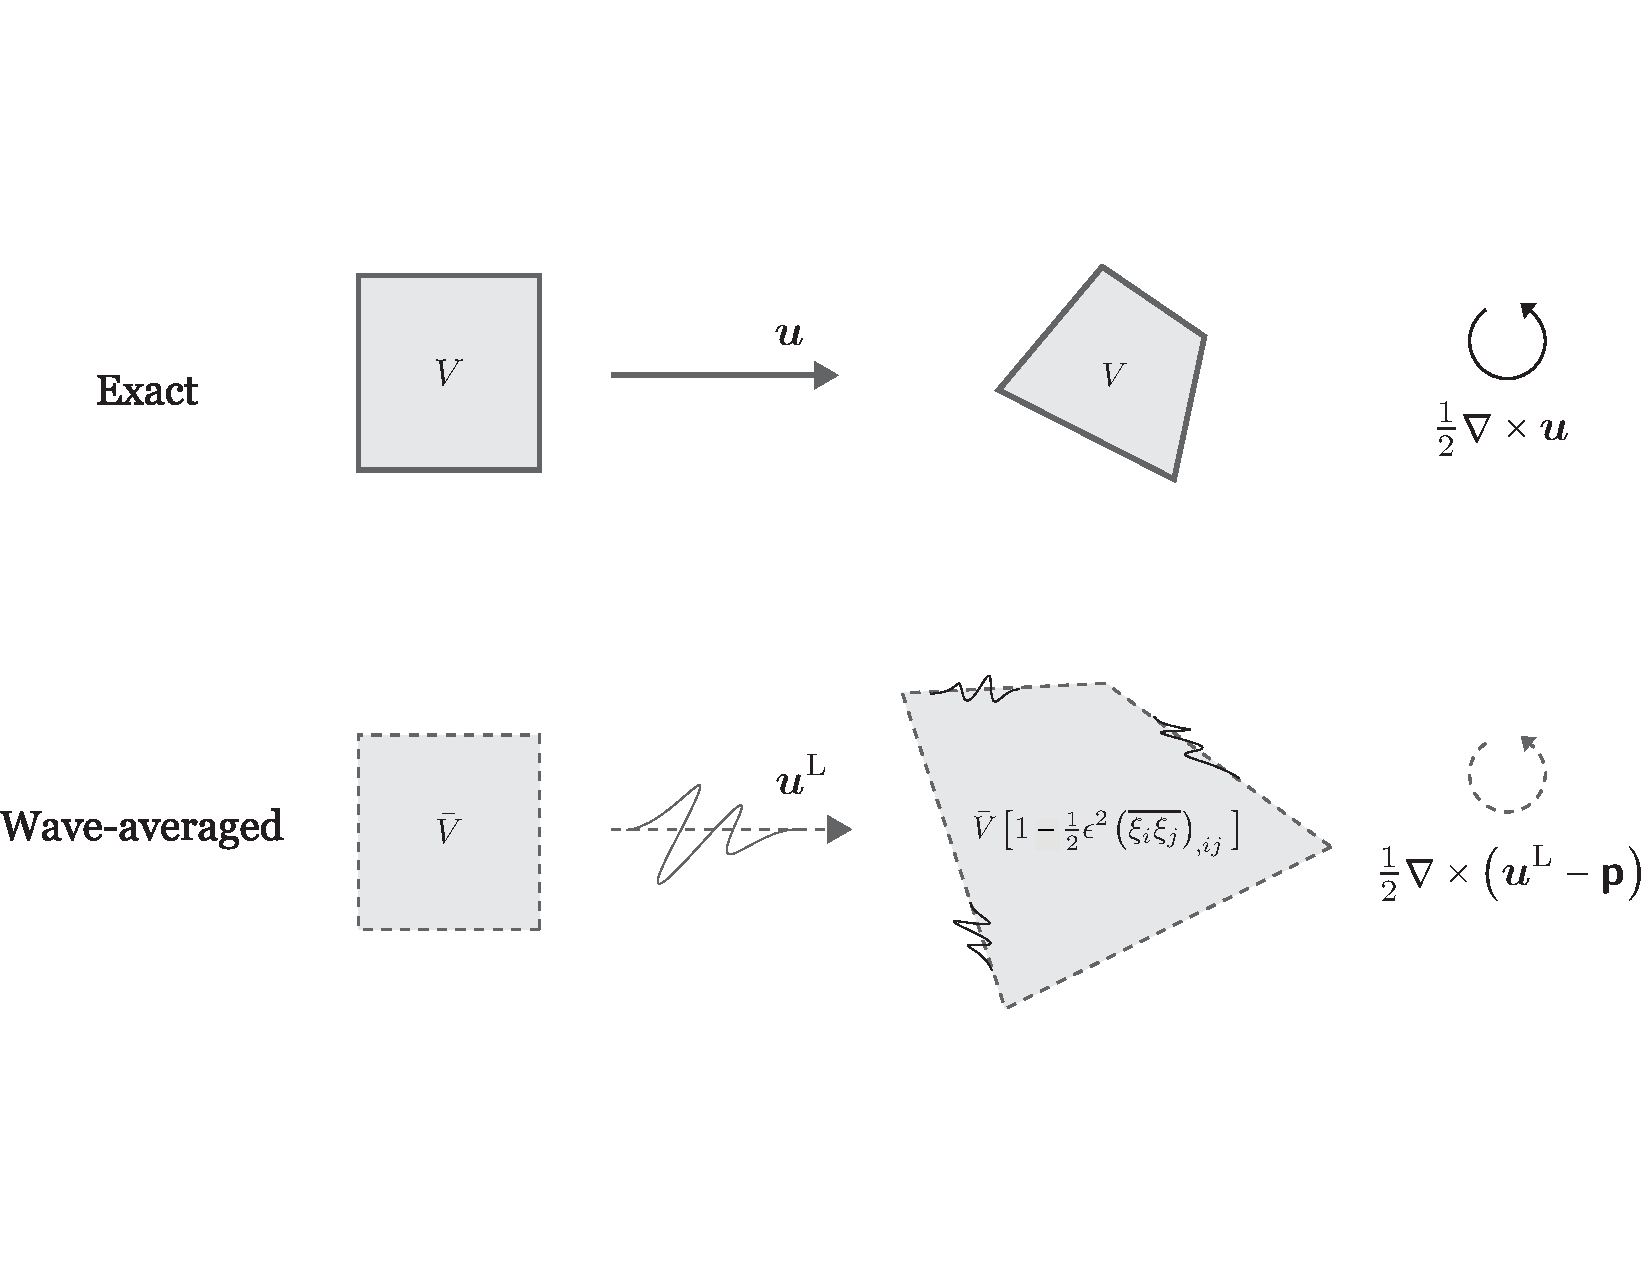
\includegraphics[width = 1\textwidth]{meanFluidElement}
\caption[Kinematics of exact and wave-averaged fluid elements.]{Kinematics of exact and wave-averaged fluid elements.  The time-averaged rotation rate and volume of wave-average fluid elements contain contributions that depends solely on the spatial structure of the zero-average oscillatory field and thus cannot be calculated solely from knowledge of the average particle trajectories represented by $\buL$.  The contributions are purely kinematic in that they do not depend on the particular physics of the oscillatory field.  If the oscillatory field is divergent, its contribution to wave-averaged volume is given by the three Jacobians in \eqref{waveAveragedVolume2} rather than $\half \left ( \xi_i \xi_j \right )_{,ij}$.}
\label{meanFluidElements}
\end{figure}

\subsection{Dilation of wave-averaged fluid elements}
\label{waveAveragedVolumes}

The average volume of a wave-averaged fluid element is
\beq
V = \overline{ \int_{\wavyc} \dd \tilde V } \com
\eeq
where $\dd \tilde V$ is an infinitesimal volume in the unaveraged and exact fluid element.  To evaluate this integral in terms of coordinates in the wave-averaged fluid element we use the coordinate transformation
\beq
\dd \tilde V = \frac{\p \left ( \bx + \ep \, \bxi \right )}{\p \left ( \bx \right )} \dd \bar V \com
\eeq
where $\dd \bar V$ is an infinitesimal volume in the wave-averaged fluid element.  With this transformation, $V$ becomes
\begin{align}
V &= \int_{\meanc} \overline{ \frac{\p(x+\ep \, \xi,y+\ep \,  \eta,z+\ep \,  \zeta)}{\p(x,y,z)} } \id \bar V \com \\
&= \int_{\meanc} \overline{ \Bigg [ 1 + \ep \, \bnabla \bcdot \bxi + \ep^2 \left ( \frac{\p (\xi,\eta)}{\p(x,y)} +  \frac{\p (\xi,\zeta)}{\p(x,z)} +  \frac{\p (\eta,\zeta)}{\p(y,z)} \right ) + \cdots \Bigg ] } \id \bar V \com \label{waveAveragedVolume2} \\
&= \int_{\meanc} 1 - \ep^2 \half \left ( \overline{ \xi_i \xi_j } \right )_{,ij} \id \bar V \per
\end{align}
The last step converting the three Jacobians into the compact form $\half \left ( \overline{\xi_i \xi_j} \right )_{,ij}$ uses $\left ( \bnabla \bcdot \bxi \right )^2 = 0$.  

This calculation implies the volume of the mean fluid element is given by
\beq
V \approx \bar V \left ( 1 - \ep^2 \half \left ( \overline{\xi_i \xi_j} \right )_{,ij} \right ) \com
\eeq
where $\bar V$ is the volume calculated naively by direct inspection of the wave-averaged particle trajectories.  As in the case of wave-averaged fluid element rotation, observations of the wave-averaged position of fluid particles expressed by knowledge of $\buL$ are insufficient to determine the volume of the wave-averaged fluid element.  The volumetric fraction $\half \left ( \overline{\xi_i \xi_j } \right )_{,ij}$ is `hidden' by time-averaging.

\section{Wave-induced mean motion}
\label{examples}

The  wave-averaged PV in \eqref{QGconnect} implies that internal waves induce balanced mean flows.  We illustrate this by considering a scenario in which a wave packet propagates into previously quiescent fluid with $\beta=0$ and zero APV, or $q=0$.  With $q=0$ in the undisturbed state, the PV equation \eqref{QGlike} reduces to
\beq
\left ( \hlap + \L \right ) \psi = - \qdag \per
\label{meanMotion}
\eeq
Equation \eqref{meanMotion} is an elliptic equation which determines the mean streamfunction, $\psi$, induced by an arbitrary hydrostatic internal wave field associated with the vorticity source $\qdag$ defined in \eqref{wavyQ2}.  The wave-induced mean motion satisfies wave-averaged geostrophic balance, has no APV, and is slaved to the wave field.   An expanded form of $\qdag$ is
\beq
\begin{split}
\qdag =  \overline{ \sJ(u,\xi) } &+ \overline{ \sJ(v,\eta) } + f_0 \overline{ \sJ(\xi, \eta) } \\
+  \frac{f_0}{2} &\Big [  \big ( \overline{\xi^2} \big )_{xx} +  \big ( \overline{\eta^2} \big )_{yy} +  \big ( \overline{\zeta^2} \big )_{zz} + 2 \big ( \overline{\xi \eta} \big )_{xy} + 2 \big ( \overline{\xi \zeta} \big )_{xz} +2  \big ( \overline{\eta \zeta } \big )_{yz} \Big ] \per
\end{split}
\label{qwexpanded}
\eeq 
The subscript `0' on wave fields will be omitted for the remainder of this paper.  

We investigate the consequences of \eqref{meanMotion} by contrasting $\psi$ and $\buL$ induced in a vertically-bounded domain by a vertically-propagating plane wave packet (`plane') with $\psi$ and $\buL$ induced by a horizontally-propagating wave packet with mode-one vertical structure (`mode').  The planar and modal wave packets we consider are visualized in figure \ref{twoWavePackets}.

\begin{figure}
\centering
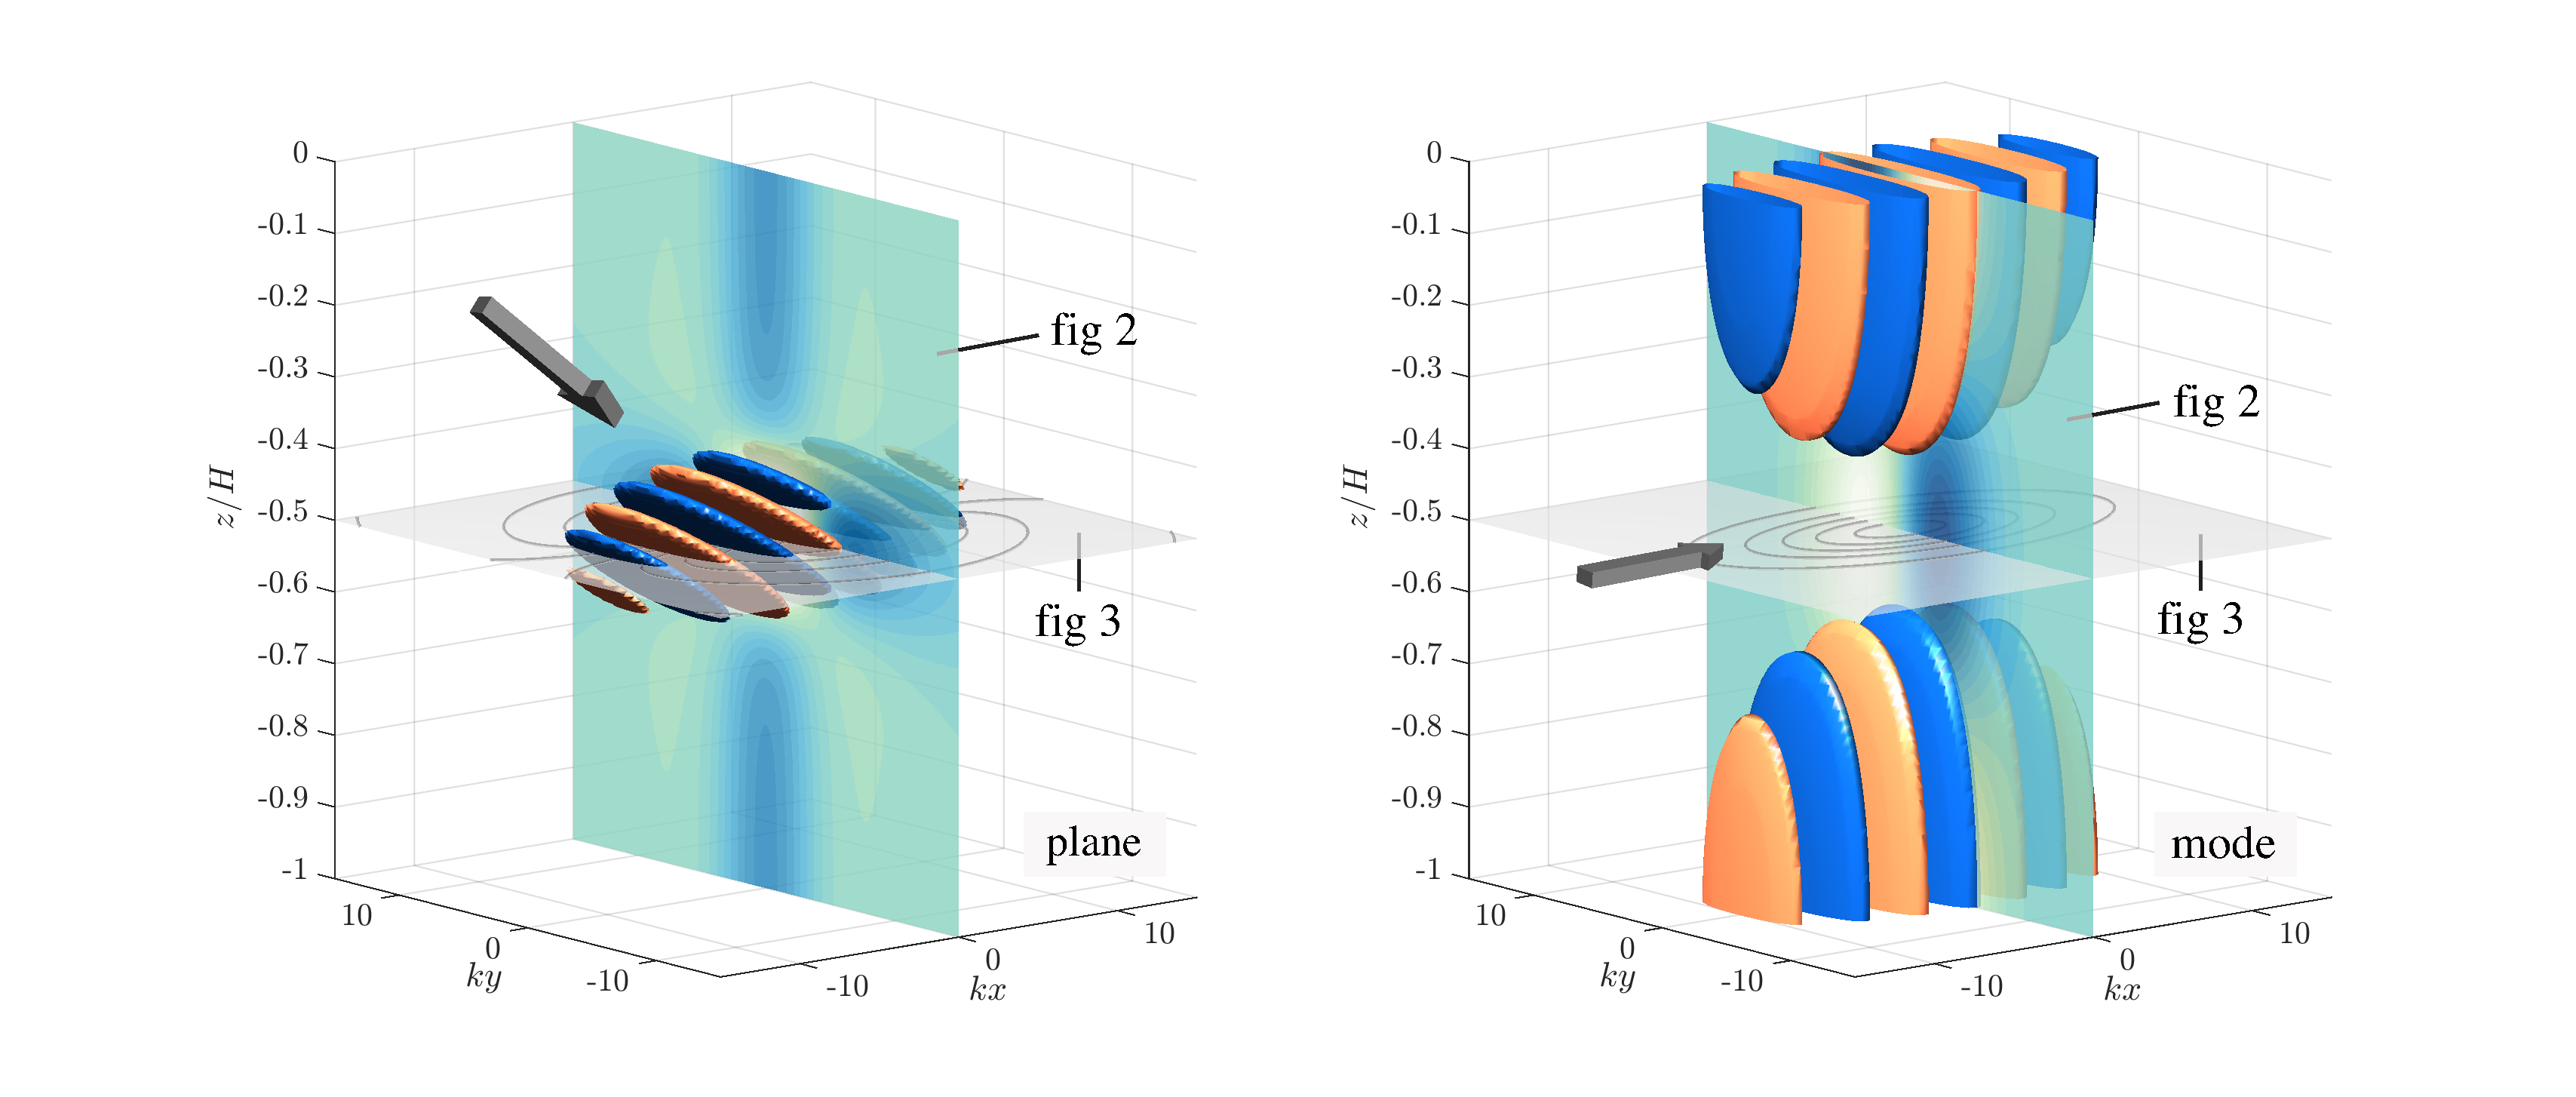
\includegraphics[width = 1\textwidth]{twoWavePackets}
\caption[Visualization of the vertically-propagating plane wave (left) and horizontally propagating mode-one wave (right)]{Visualization of the vertically-propagating plane wave (left) and horizontally propagating mode-one wave (right) with isosurfaces of pressure, $p$, at 0.325 and -0.325 of its maximum value.  Wave fields are listed in table \ref{expressions}.  A surface in the $yz$-plane show the magnitude of wave-induced $\uL$ plotted in figure \ref{inducedFlow_xz}.  A surface in the $xy$-plane shows streamlines of $\buL$ plotted in figure \ref{inducedFlow_xy}.    Gray arrows indicate the direction of wave group propagation.  Physical parameters are $f_0=10^{-4} \, \mathrm{s^{-1}}$,  $N = 2\times 10^{-3} \, \mathrm{s^{-1}}$, $\sigma = 2 f_0$, $H = 4 \times 10^{3} \, \mathrm{m}$.  The plane wave vertical wavenumber is $m=(16\pi H)^{-1}$, the horizontal wavenumbers are $k = m f_0 \sqrt{3} / N$  for the plane wave and $k = \kappa_1 \sqrt{3} = \pi \sqrt{3} f_0 / N H$ for the mode, and the scale-separation parameter is $\mu = (\ell k)^{-1} = (h m)^{-1} =1/4$.}
\label{twoWavePackets}
\end{figure}

\subsection{The Bretherton flow: mean motion induced by a vertically-propagating plane wave}

\cite{Bretherton} considered the mean motion induced by a vertically-propagating plane internal wave packet in a non-rotating fluid. Here, we consider the rotating case by solving \eqref{meanMotion}.  The pressure field associated with the plane wave packet is
\beq
p  \, \big |_{\mathrm{plane}}  \, = \; a(x,y,z,t) \, \cos (kx + mz - \sigma t) \com 
\label{packet}
\eeq
where $k$ and $m$ are horizontal and vertical wavenumbers, $\sigma$ is frequency, and $a$ is a three-dimensional envelope function with horizontal scale $\ell$ and vertical scale $h$.  The scale-separation parameter is
\beq
\mu \defn \frac{1}{k\ell} \per
\label{slowlyvarying}
\eeq
We assume $a$ is slowly varying so that $\mu \ll 1$ and $(hm)^{-1} \sim \mu \ll 1$.

Because $\mu \ll 1$, we drop $y$-derivative terms from \eqref{xmom3} through \eqref{cont3} to compute $\bu$, $\bxi$, and $b$ associated with $p$ in \eqref{packet}.  These expressions are accurate to $O(\mu)$ and listed in table \ref{expressions}.  A particularly useful result is the reduction of \eqref{ymom3} to
\beq
v+ f_0 \xi = O(\mu v)\per
\label{ymom71}
\eeq
With $\bu$ and $\bxi$, we compute $\qdag$ to leading-order in $\mu$.  Assuming $\sigma /f_0 = O(1)$, the slow variation of $a$ in $x$, $y$ and $z$  implies that 
\beq
\frac{ f_0 \left ( \overline{\xi_i \xi_j} \right )_{,ij}}{\overline{\sJ(u,\xi)}} \sim \mu \per
\eeq
Using \eqref{ymom71}, the three Jacobian terms in \eqref{qwexpanded} scale with
\beq
 \frac{\overline{\sJ(v + f_0\xi, \eta)}}{\overline{\sJ(u,\xi)}} \sim  \mu \per \label{bigFrac}
\eeq
  Thus, neglecting the eight  $O(\mu)$ terms in \eqref{qwexpanded}, the wave-averaged PV contribution $\qdag$ associated with \eqref{packet} reduces to 
\begin{align}
\qdag \, \big |_{\mathrm{plane}} &\approx \overline{ \sJ(u,\xi) } \com \\
&\approx a \, a_y \,\frac{m^4 \sigma}{k N^4} \per 
\label{qwpacket}
\end{align}
This is the conclusion  reached by BM in their equation (9.22).

We make the implications of \eqref{qwpacket} concrete by picking the envelope
\beq
a \, \big |_{\mathrm{plane}}  = A \, \exp \left[ - \left ( x / 2 \ell \right )^2 - \left ( y / \ell \right )^2 - \big ( [z+H/2] / h \big )^2 \, \right ]  \per
\label{envpacket}
\eeq
We solve \eqref{meanMotion} for $\psi$ given \eqref{envpacket} and \eqref{qwpacket} in a horizontally-periodic and vertically-bounded domain with a spectral method, using Fourier collocation in $(x,y)$ and modal collocation in $z$ with constant-$N$ vertical modes $\h_n = \cos \left ( n \pi z / H \right )$.  The left panel of figure \ref{twoWavePackets} visualizes the wave field associated with \eqref{envpacket} and the caption of figure \ref{twoWavePackets} lists the physical parameters used to make figures \ref{twoWavePackets} through \ref{inducedFlow_xy}.

\begin{table}
%\hrule \vspace{2ex}
\caption[Pressure, buoyancy, velocity, particle displacements, and $\qdag$ for mode-one and vertically-propagating plane wave fields. ]{Pressure, buoyancy, velocity, particle displacements, and $\qdag$ for mode-one and vertically-propagating plane wave fields.  The symbol $\approx$ is used for relationships that hold to leading-order in $\mu$. \vspace{-2.5ex}}
\begin{center}
\begin{tabular}{r c l c | c r c l} 
\multicolumn{3}{c}{\it vertically-propagating plane wave field}& \hspace{-0.5ex} & \hspace{-0.5ex} & \multicolumn{3}{c} {\it mode-one wave field} \\[2ex]
$\theta$ &$\defn$& $kx + mz - \sigma t$								& & &
$\phi$ &$\defn$& $kx - \sigma t$									\\[1ex]
$a$ &=&  $ A \, \ee^{ -(x / 2 \ell)^2 - (y/\ell)^2 - \left ( [z+H/2]/h \right )^2}$		& & &
$a$ &=&  $ A \, \ee^{ -(x / 2 \ell)^2 - (y/\ell)^2 }		$					\\[1ex]
$p$ &=&   $ a \, \cos \theta$ 										& & &
$p$ &=&	$ a \, \h_1 \cos \phi$ 	 									\\[1ex]
$u$ &$\approx$&   $ a  \, \frac{m^2 \sigma}{k N^2} \cos \theta $  			& & &
$u$ &$\approx$&	$ a \, \frac{\sigma \kappa_1^2}{k f_0^2} \h_1 \cos \phi $	\\[1ex]
$- f_0 \xi = \, v$ &$\approx$& $ a \, \frac{m^2 f_0}{k N^2} \sin \theta$  			& & &
$- f_0 \xi = \, v$ &$\approx$& $  a \, \frac{\kappa_1^2}{k f_0} \h_1 \sin \phi $  	\\[1ex]
$w$ &$\approx$&  $ - a \, \frac{m \sigma}{N^2} \cos \theta$ 				& & &
$w$ &$\approx$&	$ -a \, \frac{\sigma}{N^2} \h_1' \sin \phi $ 				\\[1ex]
$- \zeta N^2 = \, b$ &$\approx$& $-a \, m \, \sin \theta $  		 			& & &	
$- \zeta N^2 = \, b$ &=& $ a \, \h_1' \cos \phi$							\\[1ex]
$\eta$ &$\approx$& $ a \, \frac{m^2 f_0}{k N^2 \sigma} \cos \theta 	$  		& & &	
$\eta $ &$\approx$& $ a \, \frac{\kappa_1^2}{k  f_0 \sigma} \h_1 \cos \phi$	\\[1ex] 
$\qdag$  &$\approx$& $\left  (\half a^2 \right )_{\! y} \, \frac{m^4 \sigma}{k N^4} $& & &
$\qdag $ &$\approx$& $a^2 \, \frac{\kappa_1^2}{2 f_0^3} \, \L \big [ \half \h_1^2 \big ]$
\end{tabular}
\end{center}
\label{expressions}
%\hrule
\end{table}


The mean motion implied by \eqref{envpacket} and \eqref{qwpacket} is depicted in figures \ref{inducedFlow_xz} and \ref{inducedFlow_xy}.  The left panel in figure \ref{inducedFlow_xz} plots $\uL$ on a vertical plane in $(y,z)$ which divides the plane wave packet, revealing the dipolar horizontal structure of $\uL$ and its vertical coincidence with the wave envelope.  The top left panel of figure \ref{inducedFlow_xy} plots streamlines of $\buL$ in an $xy$-plane at $z=-H/2$, showing that the plane-wave $\buL$ resembles a vortex dipole in the horizontal.  Color-filled contours indicate the magnitude of $\buL$ and a dotted line outlines the plane wave envelope.

The top right panel of figure \ref{inducedFlow_xy} compares the $x$-components of the Lagrangian-mean $\buL$ and Stokes velocity $\buS$ on a line in $y$ through $(x,z) = (0,-H/2)$.  The $x$-component of $\buS$ defined in \eqref{stokesDefn} is
\beq
\uS \defn \overline{ \bxi \bcdot \bnabla u } = \overline{\xi u_x } + \overline{\eta u_y} + \overline{ \zeta u_z} \per
\label{uSdefn}
\eeq
Integration by parts and use of $u_x \approx - w_z$ implies that $\overline{\xi u_x}+\overline{\zeta u_z} \approx \left ( \overline{u \zeta} \right )_{\! z}$, and $\left ( \overline{u \zeta} \right )_{\! z} \approx O(\mu \zeta u_z)$ follows from the quadrature of $u$ and $\zeta$ for the packet.  Thus
\begin{align}
\uS \, \big |_{\mathrm{plane}} &\approx \overline{\eta u_y} \com \\
&\approx a \, a_y \, \frac{m^4 f_0}{2 k^2 N^4} \per
\label{packetdrift}
\end{align}

The top right panel of figure \ref{inducedFlow_xy} indicates that $\uL \gg \uS$ at $(x,z)=(0,-H/2)$.  This result can be anticipated with a scaling argument.  The scaling of $\uS$ is relatively simple: because $\eta \sim f_0 u / \sigma^2$ and $u_y \sim u / \ell$,
\beq
\uS  \, \big |_{\mathrm{plane}} \sim   \frac{u^2 f_0}{\sigma^2 \ell}\per
\eeq
The scaling for $\uL$ requires \eqref{meanMotion}.  Scaling terms on the left of \eqref{meanMotion} gives
\beq
\hlap \psi \sim \frac{\psi}{\ell^2} \com \qquad \text{and} \qquad \L \psi \sim \frac{f_0^2 \psi}{(Nh)^2} = \, \left ( \frac{ f_0 m}{N k} \right )^{\! 2} \frac{\psi}{\ell^2} \com
\eeq
where we have used both $\ell = (\mu k)^{-1}$ and $h = (\mu m)^{-1}$ to obtain the rightmost term.  For moderately super-inertial waves with $(f_0 m / N k)^2 \approx O(1)$, $\hlap \psi$ and $\L \psi$ scale similarly, and from \eqref{meanMotion} we obtain $\psi \sim \ell^2 \qdag$ and $\psi / \ell \sim \uL \sim \ell \qdag$.   The scaling for $\qdag$ follows more simply: with $u_x \sim k u$ and $\xi_y \sim u / \sigma \ell$ we deduce that
\beq
\qdag  \, \big |_{\mathrm{plane}} \, \sim \, \frac{u^2 \, k}{\sigma \ell} \com \qquad \text{and} \qquad \uL  \, \big |_{\mathrm{plane}} \sim \frac{u^2 \, k }{\sigma} \per
\eeq
Putting the pieces together and remembering that $k \ell = \mu^{-1}$ yields
\beq
\frac{\uL}{\uS}  \, \big |_{\mathrm{plane}} \sim \frac{\sigma}{\mu f_0} \per
\eeq
The plane-wave Lagrangian-mean flow is $O(\mu^{-1})$ larger than the Stokes velocity and the Eulerian mean flow is $\avu \approx \uL$ to leading-order in $\mu$.


\subsection{Mean motion induced by a vertical mode-one internal wave}

We contrast the plane-wave-induced  mean motion with the flow induced by a domain-filling, vertical mode-one internal wave.  In an ocean of depth $H$, the vertical modes are the eigenfunctions $\h_n(z)$ that satisfy 
\beq
\L \h_n + \kappa_n^2 \h_n = 0 \qquad \text{with} \qquad \h_n' = 0 \quad \text{at} \quad z=0 \text{ and } z = -H \label{vm1} \com
\eeq
where $\kappa^{-1}_n$ is the Rossby deformation length for mode-$n$ and $\L$ is the second-order linear operator defined in \eqref{eq1}.  When $N$ is constant, the vertical modes are $\h_n = \cos (n \pi z / H)$ with deformation length $\kappa_n^{-1} = N H / n \pi f_0$.   We consider a mode-one wave pressure field of the form
\beq
p \, \big |_{\mathrm{mode}}  \, = \; a(x,y,t) \, \h_1(z) \cos( kx - \sigma t) \com 
\label{mode}
\eeq
where $k$ is horizontal wavenumber, $\sigma$ is frequency, and $a$ is a slowly-varying envelope function with horizontal scale $\ell$.  We assume $ 1 / k \ell = \mu  \ll 1$ as in \eqref{slowlyvarying}, which permits easy computation of $\bu$, $\bxi$, and $b$ given in table \ref{expressions} from equations \eqref{xmom3} through \eqref{cont3}. 

With $\bu$ and $\bxi$ we compute the mode-one $\qdag$ to leading-order in $\mu$.  The mode-one vertical structure implies the terms in \eqref{qwexpanded} scale differently than for the plane wave.  In particular, 
\beq
\frac{\overline{ \sJ(u,\xi)} }{ \text{\raisebox{2.5ex}{\,}} \quad  f_0 \big ( \overline{\zeta^2} \big )_{\! zz} } \sim \mu \per
\eeq
Moreover, because  \eqref{ymom71} and \eqref{bigFrac} apply also for the mode, none of the Jacobian, pseudomomentum-associated terms contribute to $\qdag$ at leading-order.  Among the remaining terms on the second line of \eqref{qwexpanded}, the assumptions $\mu \ll 1$ and $\sigma / f_0 = O(1)$ imply
\beq
\frac{ \big ( \overline{\eta \zeta} \big)_{\! yz}}{ \text{\raisebox{2.5ex}{\,}} \big (\overline{\zeta^2} \big)_{\! zz} } 
\sim \mu 
\qquad \text{and} \qquad 
\frac{ \big ( \overline{\xi^2 }\big)_{\! xx} + \big (\overline{\eta^2} \big)_{\! yy}}{ \text{\raisebox{2.5ex}{\,}} \big (\overline{\zeta^2} \big)_{\! zz}} 
\sim \mu^2 \per
\eeq
Finally, the quadrature of $\left ( \xi,\zeta \right )$ and $\left ( \eta, \xi \right )$ and the fact that $\mu \ll 1$ imply 
\beq
\frac{ \left ( \overline{\xi \zeta} \right )_{\! xz} + \left ( \overline{\eta \xi} \right )_{\! xy} }{ \text{\raisebox{2.5ex}{\,}} \big (\overline{\zeta^2} \big)_{\! zz} } \sim \mu^2 \per
\eeq
The only survivor at leading-order from $\qdag$ in \eqref{qwexpanded} is therefore $\half f_0 (\overline{\zeta^2})_{zz} $, and the mode-one $\qdag$ is 
\begin{align}
\qdag \, \big |_{\mathrm{mode}} &\approx \half f_0  \big ( \overline{\zeta^2} \big )_{\! zz} \, \, \com \label{qwReduced} \\
&\approx - a^2 \, \frac{\kappa_1^2}{2 f_0^3} \, \L \big [ \half \h_1^2 \big ] \per
\label{qwMode1}
\end{align}
The final expression in \eqref{qwMode1} is found using $\zeta$ from table \ref{expressions} along with $\L \h_1 = - \kappa_1^2 \h_1$.  For a slowly-varying mode-$n$ wave, $\qdag$ follows by replacing `1' with `$n$' in \eqref{qwMode1}. 

We investigate the consequences of \eqref{qwMode1} by choosing the envelope
\beq
a \,  \big |_{\mathrm{mode}} = A \, \exp \left [ - \left  (x/2\ell \right )^2 - \left ( y/\ell \right )^2 \right ] \per
\label{envmode1}
\eeq
As for the vertically-propagating plane wave, we solve \eqref{meanMotion} for $\psi$ with $\qdag$ determined by   \eqref{envmode1} and \eqref{qwMode1} using a spectral method.  For the mode-one wave with constant $N$, $\psi$ is mode-two and thus proportional to $\cos(2 \pi z / H)$.  The wave field associated with \eqref{envmode1} is visualized in the right panel of figure \ref{twoWavePackets} and the mean motion it induces is illustrated in figures \ref{inducedFlow_xz} and \ref{inducedFlow_xy}.

\begin{figure}
\centering
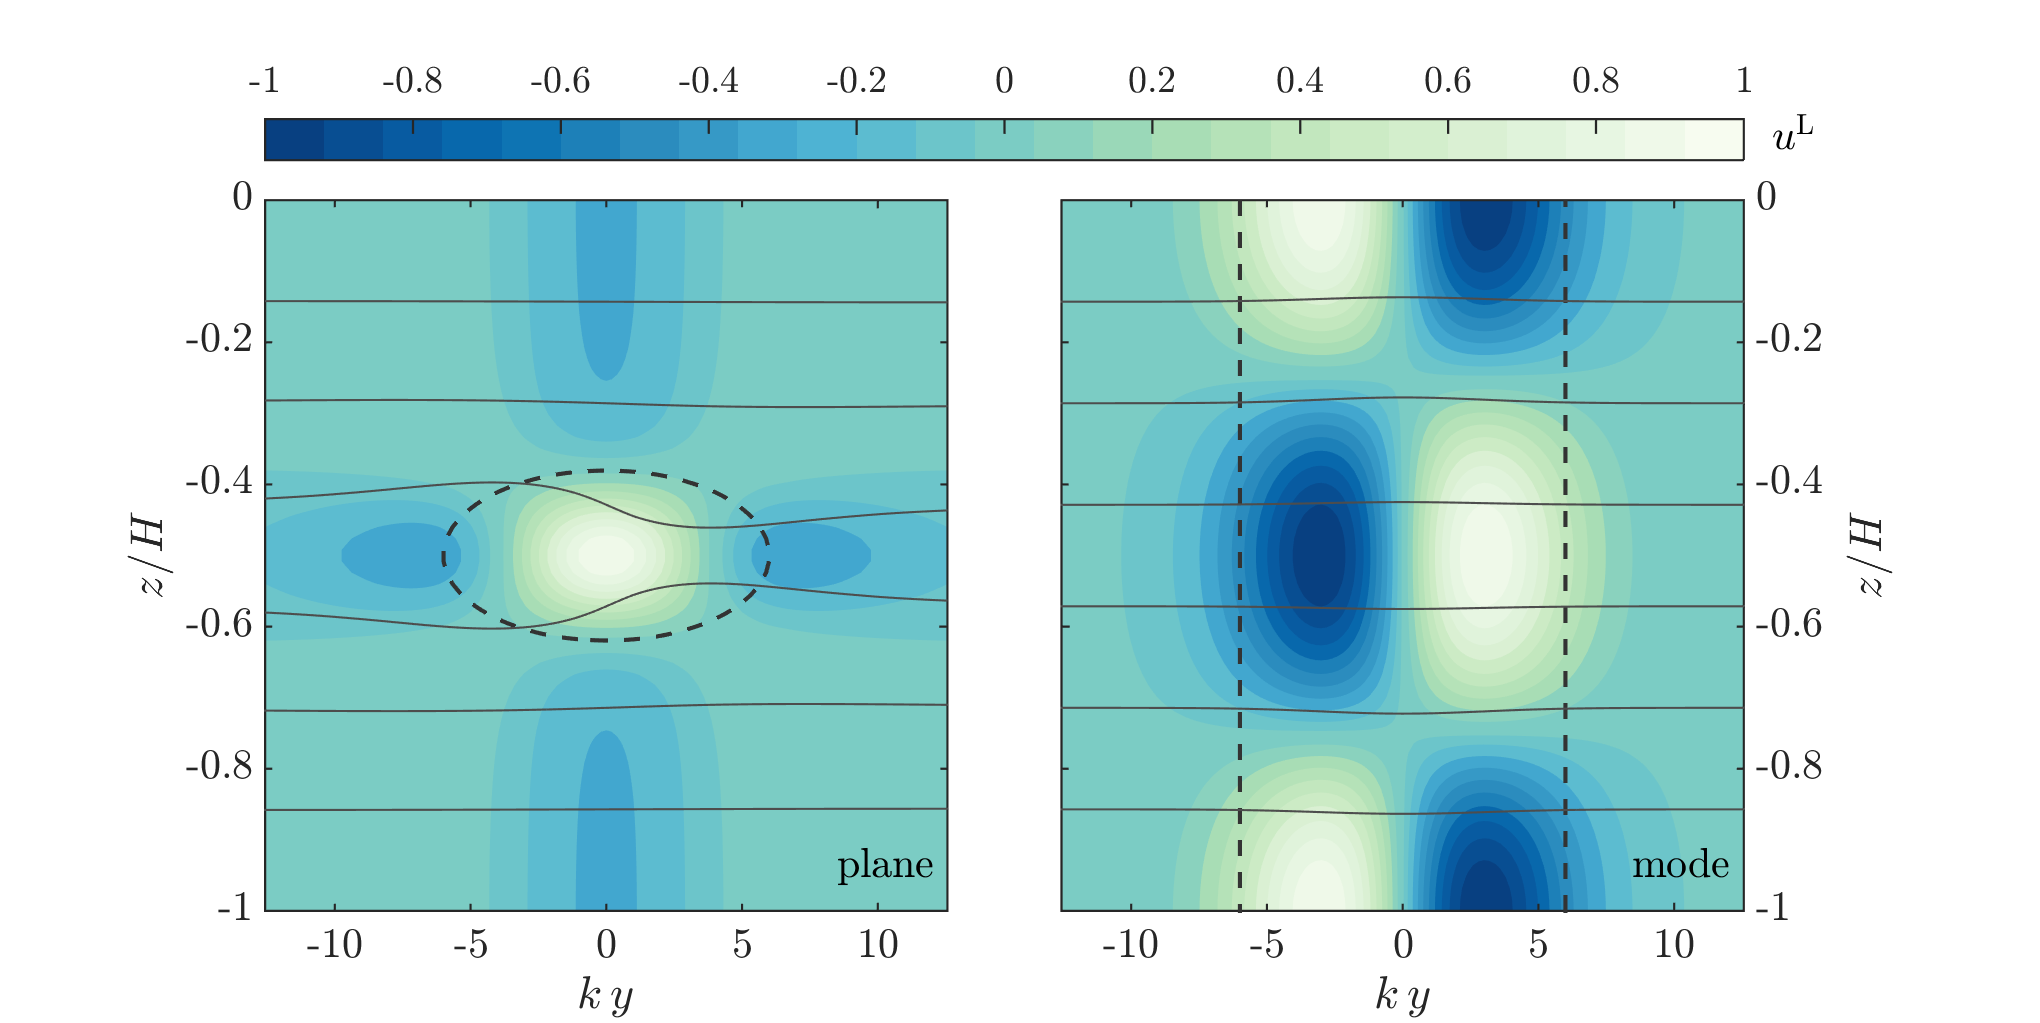
\includegraphics[width = 1\textwidth]{inducedFlow_xz}
\caption[Vertical structure of wave-induced mean flows]{Vertical structure of wave-induced mean flows at $x=0$ for vertically-propagating plane wave (left) and vertical mode-one wave (right).  Color-filled contours show $\uL=-\psi_y$ normalized by its extreme value, isopycnals are in light gray, and dark gray dashed lines show wave envelopes with contours of $\half a$.  The plane wave packet induces a dipolar $\uL$ while the mode-one wave induces a monopolar, mode-two eddy-like $\uL$. Parameters are listed in the caption of figure \ref{twoWavePackets}.}
\label{inducedFlow_xz}
\end{figure}

The right panel of figure \ref{inducedFlow_xz} shows the mode-two vertical structure of $\buL$, and the bottom left panel of figure \ref{inducedFlow_xy} reveals the horizontally compact and monopolar form of $\buL$.  The bottom right panel of figure \ref{inducedFlow_xy} compares $\uL$ with the Stokes velocity correction $\uS$ for the mode-one wave, where $\uS$ is defined in \eqref{stokesDefn} and \eqref{uSdefn}.  Unlike  the plane-wave $\uS$ in \eqref{packetdrift}, in the mode-one wave field $(\overline{u \zeta})_{ z}$ is larger than $\overline{\eta u_y}$ by $O(\mu)$, and thus
\begin{align}
\uS \,  \big |_{\mathrm{mode}} &\approx \left ( \overline{u \zeta} \right )_{\! z} \com \\
&\approx - a^2 \, \frac{\sigma \kappa_1^2}{2 k f_0^4} \, \L \big [ \half \h_1^2 \big ] \per 
\end{align}
The Stokes velocity correction does not involve spatial derivatives of the envelope $a(x,y,t)$.

\begin{figure}[H]
\centering
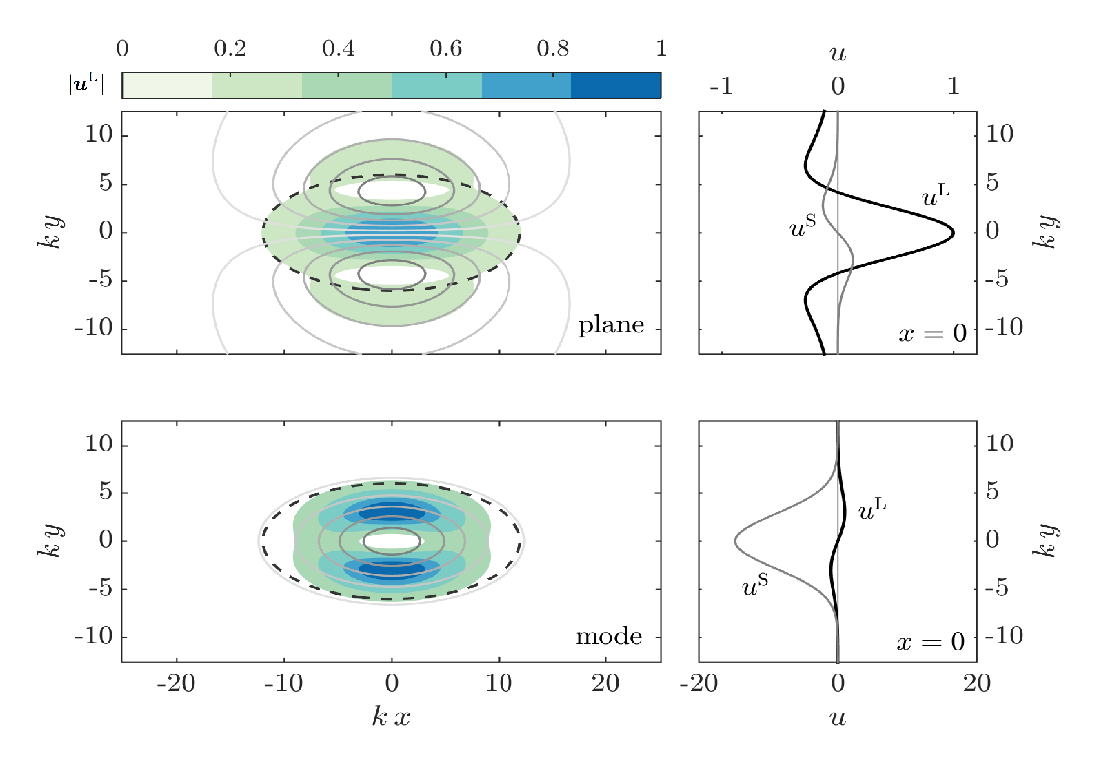
\includegraphics[width = 1\textwidth]{inducedFlow_xy}
\caption[Horizontal structure of wave-induced mean flows]{Horizontal structure of wave-induced mean flows in a top-down $xy$-view at $z=- H/2$ associated with the vertically-propagating plane wave (top) and vertical mode-one wave (bottom).  At left, solid gray lines are streamlines of $\buL$,  color-filled contours show normalized flow magnitude $| \buL |$, and dark gray dashed lines show wave envelopes with contours of $\half a$.  At right $\uL$ and $\uS$ are plotted versus $y$ on a line at $(x,z)=(0,-H/2)$, both normalized by the maximum magnitude of $\uL$.  The $x$-axes of the right panels are different for mode and plane wave: $\uL$ dominates for the plane wave, while $\uS$ dominates for the mode-one wave.  Parameters are listed in the caption of figure \ref{twoWavePackets}.}
\label{inducedFlow_xy}
\end{figure}

The bottom right panel of figure \ref{inducedFlow_xz} indicates that $\uS \gg \uL$ at $(x,z)=(0,-H/2)$ for the mode-one wave: the reverse relationship found for the plane-wave case.  This fact can be deduced with a scaling argument.  First, $\xi \sim u / \sigma$ and $\zeta_z \approx - \xi_x$ implies $\zeta \sim H k \xi$, such that
\beq
\uS  \, \big |_{\mathrm{mode}} \sim  \frac{k u^2}{\sigma} \per
\eeq
That the mode $\uS$ scales with $k$ rather than $1/\ell$ contrasts with the plane-wave case.  Next, from \eqref{meanMotion},
\beq
\hlap \psi \sim \frac{\psi}{\ell^2} \com \qquad \text{but} \qquad \L \psi \sim \kappa_1^2 \psi = \frac{1}{(\mu \ell)^2} \left ( \frac{\kappa_1}{k} \right )^{\! 2} \psi \per
\eeq
Assuming moderately super-inertial waves for which $(\kappa_1/k)^2 \approx O(1)$, we conclude that $\L \psi$ is $O \left ( \mu^{-2} \right )$ {\it larger} than $\hlap \psi$.  Therefore, $\psi \sim (\mu \ell)^2 \qdag$ and $\psi / \ell \sim \uL \sim \mu^2 \ell \qdag$.  Again using the fact that $\zeta \sim H k \xi$, we then find
\beq
\qdag \, \big |_{\mathrm{mode}} \sim f_0 \left ( \frac{k u}{\sigma} \right )^{\! 2} \com \qquad \text{and} \qquad \uL \, \big |_{\, \mathrm{mode}}  \sim \frac{\mu \, u^2 \, k f_0}{ \sigma^2} \per
\eeq
Dropping the parts into place yields 
\beq
\frac{\uL}{\uS} \: \Big |_{\, \mathrm{mode}} \sim \frac{\mu \, f_0}{ \sigma} \com
\eeq
which means the Lagrangian-mean flow is $O(\mu)$ smaller than the Stokes velocity field.  This implies further that, to leading-order in $\mu$, the Eulerian-mean flow is
\beq
\avu \approx - \uS \per
\label{antiStokes}
\eeq
This Eulerian-mean $\bar u$ is an ``anti-Stokes flow''.  The Lagrangian-mean flow, which is relevant for potential vorticity advection, is a small residual remaining after the large cancellation in \eqref{antiStokes} and is $O(\mu)$ smaller for the mode-one wave than for the plane wave.

The fact that $\L \psi$ is much larger than $\hlap \psi$ for the mode-one wave is striking and means the primary averaged effect of slowly varying, vertical-mode waves is a slight displacement of isopycnals.  The isopycnal displacement is associated with a balanced flow when the wave field is spatially non-uniform.  Equivalent to this physical explanation is the statement that the APV equation \eqref{meanMotion} can be solved by neglecting $\hlap \psi$ and  ``cancelling the $\L$'' between $\L \psi$ and $\qdag$ in \eqref{qwMode1}.  We must subtract the barotropic part of $\h_1^2$, since the vertical average of \eqref{meanMotion} implies $\psi$ has no barotropic component.  This yields
\beq
\psi \; \approx \;  \frac{a^2 \kappa_1^2}{4 f_0^3} \Bigg [ \frac{1}{H}\int_{-H}^0 \h_1^2 \, \id z - \h_1^2 \Bigg ] \per
\label{simplePsi}
\eeq
Equation \eqref{simplePsi} is valid for general stratification profiles $N(z)$ and vertical modes $\h_n$ when the 1's are replaced by $n$'s.  For slowly-varying vertical mode waves, the streamlines of the wave-induced mean motion follow the contours of $a^2$, which explains the monopolar mode-induced motion evident in figure 3.


\section{Discussion}
\label{discussion}

The wave-QG theory in \eqref{eq1} through \eqref{eq3}, first derived for constant stratification and small-scale waves by \cite{BuhlerMcIntyre}, is a correction to standard quasi-geostrophy which accounts for the averaged effects of strong internal waves on balanced planetary flows.  The extension of wave-QG to non-constant stratification is non-trivial and motivates the introduction of a new material invariant: the available potential vorticity, or APV.  APV is on one hand a useful computational tool in that it separates waves and balanced flow in Eulerian reference frames.  On the other hand, the conceptual significance of APV is suggested by the immediate emergence of QGPV from APV as the leading-order term in a low-Rossby-number expansion.

%In passing from standard QG to wave-QG, the ordinary velocity and its streamfunction are replaced by the Lagrangian-mean velocity $\buL$ and the Lagrangian-mean streamfunction $\psi$.  The two velocity fields are analogous: $\buL$ is the advective velocity in wave-averaged flow which determines wave-averaged particle trajectories and the advection of material invariants like potential vorticity.  It is $\buL$ which satisfies the wave-averaged geostrophic balance condition, which physically reflects the fact that the Coriolis ``force'' is fundamentally an advective term.  We stress that, despite its name, the Lagrangian-mean velocity is an {\it Eulerian} quantity.

The effect of internal waves on balanced flow is expressed concisely in $\qdag$, the wave contribution to potential vorticity in \eqref{eq3}.  We identify two distinct parts of $\qdag$: the vertical component of `pseudovorticity,' $\bzh \bcdot \curl \sbp$, and wave-averaged vortex stretching $\half f_0 ( \overline{ \xi_i \xi_j } )_{,ij}$.  Both terms have essentially kinematic origins.  As shown in section 10.2.7 of \cite{Buhler}, pseudovorticity is a relative vorticity term which appears in wave-averaged circulation integrals over a material contours in {\it arbitrary} oscillatory flow.  Equivalently, it arises in the wave-averaged integral of vorticity over a material surface.  
%Pseudovorticity, therefore, can be interpreted fundamentally as a ``hidden'', or wave contribution to local vorticity of a wave-averaged fluid: it is {\it not} explicitly associated with the wave-averaged fluid motion, and unlike in unaveraged fluid dynamics, vorticity in a wave-averaged fluid cannot be extracted solely from measurement of the wave-averaged flow.
Pseudovorticity, therefore can be interpreted fundamentally as the part of vorticity which is `hidden' by wave averaging: the total vorticity is the sum of the vorticity of wave-averaged velocity, $\hlap \psi$, minus the pseudovorticity $\bzh \bcdot \curl \sbp$.

Wave-averaged vortex stretching, $\half f_0 ( \overline{ \xi_i \xi_j } )_{,ij} \,$, on the other hand, is a vortex stretching term that appears in wave-averaged integrals over material volumes in oscillatory and incompressible flow.  Thus the non-divergence of exact and unaveraged particle trajectories does {\it not} ensure non-divergence for wave-averaged particle trajectories, a point which is developed clearly by \cite{McIntyre1988}.  While small compared to pseudovorticity for nearly-plane waves, wave-averaged vortex stretching is leading-order for a vertical mode-one wave, and is the only part of $\qdag$ that remains in two-dimensional flow in $(x,z)$.

%The algebraic difficulties of our derivation hashed out in appendix \ref{AppenA} and \ref{qwappendix} can be viewed as constraining these kinematic concepts to particle trajectories the satisfy the physics of the linearized hydrostatic Boussinesq system. 

The form of \eqref{eq1} through \eqref{eq3} suggests that energy transfer occurs generally between preexisting waves and preexisting mean flow, as demonstrated for near-inertial waves by \cite{XieVanneste}.  Wave-QG also implies that wave-induced balanced flows exist even in the absence of potential vorticity, or if $q=0$ everywhere and $\psi_z=0$ at boundaries.  However, this balanced flow is determined instantaneously and completely by the wave field, is not associated with energy transfer from waves to balanced flow, and has no independent evolution.

A major missing piece from wave-QG is a description of slow wave evolution which couples to \eqref{eq1} through \eqref{eq3}.  
%To this point such evolution has been described only for near-inertial waves by \cite{XieVanneste}.  
A potential complication is wave-wave nonlinear interaction, which can lead to wave evolution on the time-scale $(\ep f_0)^{-1}$: slower than the wave frequency time-scale, but faster than the mean flow evolution time scale.  In this case, careful averaging is required to separate time-scales and ensure that neither $f_0^{-1}$ nor $(\ep f_0)^{-1}$ appear in \eqref{eq1} through \eqref{eq3}.  
%Interestingly, an expansion of the APV equation including $t_1$ shows that the mean flow equation over the intermediate time-scale is given simply by equation \eqref{meanMotion}.  
The complications incurred by nonlinear wave evolution reinforce the assertion that wave evolution equations are an important component of any consistent, reduced description of flows comprised of both strong waves and APV.  Strong internal waves and balanced flow cannot be considered independent superposed components of fluid motion: instead, waves and balanced flow coevolve in an interwoven system with its own unique dynamics.

%\begin{acknowledgments}
%This work was supported by the National Science Foundation under  OCE-1357047. We thank Oliver B\"uhler, Jacques Vanneste and Jin-Han Xie for helpful discussions.
%\end{acknowledgments} 
  
\begin{subappendices}

\section{Quadratic wave properties}
\label{AppenA}


In this appendix we obtain some quadratic properties of solutions to the linearized Boussinesq equations in \eqref{xmom3} through \eqref{cont3}.  To lighten the notation we suppress the subscript $0$ on all fields throughout this appendix.  This means that, within this appendix, $\bu$, $\bxi$,  $p$ and $b$ refer to the zero-order wavy fields $\bu_0$, $\bxi_0$,  $p_0$ and $b_0$ in \eqref{xmom3} through \eqref{cont3}.  We frequently use the averaging identity
\beq
\overline{\theta \phi_{\tt} } = - \overline{\theta_{\tt} \phi } \com
\label{fundIden}
\eeq
where $\phi$ and $\theta$ are any of the leading-order wave fields.  The derivation of these quadratic properties requires constant use of the definitions $\bxi_{\tt} = \bu$ and $b = - \zeta N^2$.

\subsection{The virial equation and the Stokes correction to pressure}

The virial equation is obtained by  taking the dot product of the wave momentum equations \eqref{xmom3} through \eqref{zmom3} with the particle displacement $\bxi$.  The time-average of the result is
\beq
\pS = \avbg{u^2} + \avbg{v^2} + f_0 \overline{(\xi v - \eta u)} - N^2 \avbg{\zeta^2} \com
\label{virial1}
\eeq
where the leading-order `Stokes correction' \citep{Buhler, Craik} to the pressure is
\beq
\pS \defn \avbg{ \bxi\bcdot \bnabla p}\per
\label{pSdef}
\eeq

\subsection{The `gradient virial equation'}
\label{virialgrad}

Useful identities for $\bnabla \pS$ are obtained from the spatial gradient  of the time-averaged virial equation \eqref{virial1}.  To maximally simplify this gradient, we need further linear-wave identities. Consider, for example,  the $x$-derivative of $\pS$,
\beq
\pS_x = \overline{ \bxi_x \bcdot \bnabla p } + \overline{\bxi \bcdot \bnabla p_x} \per
\eeq
It turns out that both terms on the right are equal to one another, and thus individually equal to $\half\pS_x$.  We show this by dotting wave momentum equations \eqref{xmom3} through \eqref{zmom3} with $\bxi_{x}$ and averaging over the fast time.  A crucial intermediate result involving the Coriolis terms is
\begin{align}
\avbg{v \xi_x} - \avbg{u \eta_x} &=  \p_x \left ( \avbg{v \xi} \right ) = - \p_x \left ( \avbg{u \eta} \right ) \com \\
&= \half \p_x \left ( \avbg{v \xi} - \avbg{u \eta} \right ) \per
\end{align}
Applying averaging identities and forming exact $x$-derivatives yields the desired result that $\overline{\bxi_x \bcdot \bnabla p} = \half \pS_x$, and therefore
\begin{align}
\half  \pS_x &= \avbg {\bxi_x \bcdot \bnabla p } = \avbg {\bxi \bcdot \bnabla p_x} \per
 \label{horizpg1} 
\end{align}
In similar fashion, dotting the momentum equations \eqref{xmom3} through \eqref{zmom3} with $\bxi_{y}$ and $\bxi_{z}$ produces 
\begin{align}
\half  \pS_y \; = \; \avbg {\bxi_y \bcdot \bnabla p } \; = \; \avbg {\bxi \bcdot \bnabla p_y}\com 
\label{horizpg2}
\end{align}
and 
\begin{align}
\half \pS_z \; = \; \avbg { \bxi \bcdot \bnabla p_{z} } +(N^2)_{z} \avbg{\half \zeta^2}
\; = \; \avbg {\bxi_{z} \bcdot \bnabla p} -(N^2)_{z} \avbg{\half \zeta^2}\per
\label{pluspSz}
\end{align}
As before, the second right-side identities in \eqref{horizpg2} and \eqref{pluspSz} follow from taking derivatives of $\pS$ defined in \eqref{pSdef}.  Replacing $p_z$ by $-N^2 \zeta$ in \eqref{pluspSz} produces
\beq
\half \pS_z = -N^2\left(\overline{\bxi\bcdot \grad \zeta} + \Lambda_z \overline{\half \zeta^2} \right)\per \label{vertpSgrad}
\eeq
The identities in \eqref{horizpg1} through \eqref{vertpSgrad} are handy expressions for $\grad \pS$.

\subsection{The Stokes velocity correction and wave-averaged velocity}
% $\boldsymbol{u}$} %$\bu$} % and wave-averaged velocity $\budag$}

Recall that the Stokes velocity correction is 
\begin{align}
\buS &\defn \avbg{ (\bxi \bcdot \bnabla) \bu} \per
\label{StokesAM1}
\end{align}
We turn now to the wave velocity $\budag$ defined in \eqref{udagdef} as

\beq
\budag \defn \; \underbrace{\mystrut{1.2ex} f_0^{-1} \avbg{ \bu \bcdot \bnabla v } }_{\udag}\, \bxh 
\; \; \underbrace{\mystrut{1.2ex} -f_0^{-1} \avbg{ \bu \bcdot \bnabla u} }_{\vdag}\, \byh 
\; + \; \underbrace{\mystrut{1.2ex} N^{-2} \avbg{ \bu \bcdot \bnabla b} }_{\wdag}\,  \bzh \per
\eeq
Using \eqref{fundIden} and  the leading-order buoyancy equation \eqref{buoy3}, we have
\begin{align}
\wdag &= - N^{-2} \avbg{\bxi \bcdot \bnabla b_{t}} \com \\
&=\wS \per
\label{wdagger1}
\end{align}
In contrast to $\wdag$, the horizontal components of $\budag$ are not equal to those of $\buS$.  Using the leading order $y$-momentum \eqref{ymom3}, the $x$-component of $\budag$ can be expressed as
\begin{align}
\udag &= - f_0^{-1} \avbg{\bxi \bcdot \bnabla v_{t}} \com \\
&= \uS + f_0^{-1}  \avbg{\bxi \bcdot \bnabla p_{y}} \, ;
\end{align}
 the $y$-component is $\vdag = \vS - f_0^{-1} \avbg{ \left ( \bxi \bcdot \bnabla \right ) p_{x} }$. Thus, using \eqref{horizpg1} and  \eqref{horizpg2}, we have:
\beq
\Big (\udag \com \,  \vdag \com \, \wdag \Big )  = \Big ( \uS \com \, \vS \com \, \wS \Big  )  + f_0^{-1} \Big ( \half \pS_y \com  \, \half \pS_x \com \, 0 \Big ) \per \label{weird} 
\eeq
The relationship between the three-dimensional solenoidal vectors $\buS$ and $\budag$ is expressed concisely as $ \budag = \buS + f_0^{-1} \curl \left ( \half \pS \bzh \right )$.


\section{The wave contribution to APV, $\qdag$ \label{qwappendix}}

In this appendix we summarize various expressions for the wave contribution to PV, 
\beq
\qdag \defn \frac{\avbg{ \bomega \bcdot \bnabla b }}{N^2} - \vS_x + \uS_y - \left ( \frac{f_0 \half \pS_z}{N^2} \right )_{\dz} - f_0 \Lambda_{zz}\avbg{\half  \zeta^2} \com
\label{veq1}
\eeq
introduced in \eqref{wavyQ1}.  The subscript $0$ on leading-order wave fields is suppressed throughout this appendix.  We use various wave identities from appendix \ref{AppenA}.    

Using the expression for $\pS$ in \eqref{vertpSgrad}, we have
\beq
\left ( \frac{f_0 \half \pS_z}{N^2} \right )_{\dz} = - \omS -f_0 \overline{\bxi_z \bcdot \grad \zeta}-f_0 \left(\Lambda_z \avbg{\half \zeta^2}\right)_{\dz} \com
 \label{veq2}
\eeq
where $\omS \defn \overline{\bxi \bcdot \bnabla \om}$ is the Stokes correction to the vertical vorticity.  Note that the Stokes correction vertical vorticity, $\omS$, is not equal to the vertical vorticity of the Stokes correction velocity field, $\vS_x - \uS_y$. Next, using $b=-N^2\zeta$ and $\bzh \bcdot \bomega = f_0 \zeta_z$, we find that
\beq
- \frac{\avbg{ \bomega \bcdot \bnabla b }}{N^2}= \overline{\bomega \bcdot \grad \zeta}  + f_0 \Lambda_{z} \left( \avbg{\half \zeta^2}\right)_{\dz} \per
\label{veq3}
\eeq
With the results in  \eqref{veq2} and \eqref{veq3}, and using $\bomega = - v_z \bxh + u_z \byh + f_0 \zeta_z \bzh$, we manipulate $\qdag$ in \eqref{veq1}:
\begin{align}
\qdag &= \omS -\vS_x + \uS_y + f_0 \overline{  \bxi_{z}\bcdot \grad \zeta } - \overline{\bomega \bcdot \grad \zeta}\com
\label{veq7}\\
&= \overline{\bxi_{y} \bcdot \grad u} -\overline{\bxi_{x} \bcdot \grad v} +  f_0\overline{  \bxi_{z}\bcdot \grad \zeta }  - \overline{\bomega\cdot \grad \zeta} \com  \label{veq11}\\
&=  \overline{\sJ(u,\xi)} + \overline{\sJ(v,\eta)} + f_0 \overline{ \bxi_z \bcdot \grad \zeta}\per \label{veq13}
\end{align}

With the expression for $\qdag$ in \eqref{veq13}, we are prepared to show the connection between $\qdag$ and pseudomomentum.  The pseudomomentum defined in \cite{AndrewsMcIntyre} is given to leading-order in our case by
\beq
\sp_i = - \avbg{ \xi_{j,i} \left ( u_j + \half f_0 \left (  \bzh \times \bxi \right )_j \right ) } \com 
\label{pseudomom}
\eeq
where the subscript `$,i$' denotes differentiation with respect to the $i^\th$ coordinate.  The wavy particle displacement defined here via $\bxi_{\tt} = \bu$ is equivalent at leading-order to the wavy displacement defined generally in \cite{AndrewsMcIntyre}.  The horizontal components of $\sbp$ are
\begin{align}
\sp_1 &= -\overline{\xi_x u} - \overline{\eta_x v} - \half f_0 \left(\overline{\xi \eta_x } -  \overline{\eta \xi_x }  \right)\com \label{pseudomom1} \\
 \sp_2 &= -\overline{ \xi_y u} - \overline{\eta_y v}  - \half f_0\left( \overline{\xi \eta_y } -\overline{\eta \xi_y}\right)\per
 \label{pseudomom2}
\end{align}
In passing from the definition of the pseudomomentum in \eqref{pseudomom} to \eqref{pseudomom1} and \eqref{pseudomom2} we have neglected terms  $\overline{\zeta_x w }$ and $\overline{\zeta_y w}$ which are smaller by $(H/L)^2$ than the other terms in $\sp_1$ and $\sp_2$.  This neglect is consistent with the hydrostatic approximation.

The $z$-component of the curl of the leading-order pseudomomentum, or `pseudovorticity', is
\begin{align}
\bzh \bcdot \curl \sbp &= \p_x \, \sp_2 - \p_y \sp_1 \com \\
&= \overline{\sJ(\xi,u)} + \overline{\sJ(\eta,v)} + f_0 \overline{\sJ(\eta,\xi)}  \per \label{pain7}
\end{align}
Substituting \eqref{pain7} into \eqref{veq13} we have
\beq
\qdag = - \bzh \bcdot \curl \sbp - f_0 \Big [ \overline{\sJ(\xi,\eta)} - \avbg{\bxi_z \bcdot \bnabla \zeta } \Big ] \per
\label{pain9}
\eeq
Using  $\bnabla \bcdot \bxi = \xi_x+\eta_y + \zeta_z=0$, the term in the square brackets in \eqref{pain9} can be  written as
\begin{align}
\sJ(\xi,\eta) - \bxi_z \bcdot \bnabla \zeta &= \frac{\p (\xi,\eta)}{\p(x,y)} - \bxi_z \bcdot \bnabla \zeta \com \\
&= \frac{\p (\xi,\zeta)}{\p(x,z)} - \bxi_y \bcdot \bnabla \eta \com \\
&= \frac{\p (\eta,\zeta)}{\p(y,z)} - \bxi_x \bcdot \bnabla \xi \per
\end{align}
The average of the three expressions above is
\beq
\sJ(\xi,\eta) - \bxi_z \bcdot \bnabla \zeta = \frac{1}{3} \Bigg [ \frac{\p (\xi,\eta)}{\p(x,y)} + \frac{\p (\xi,\zeta)}{\p(x,z)} +  \frac{\p (\eta,\zeta)}{\p(y,z)} \Bigg ] - \tfrac{1}{3} \xi_{i,j} \xi_{j,i} \per
\eeq
Further, using $\left ( \diver \bxi \right )^2 = 0$, we find 
\begin{align}
\xi_{i,j} \xi_{j,i} &= \left(\xi_i\xi_j\right)_{,i j} \com \label{meansq1} \\
&=- 2\Bigg [ \frac{\p (\xi,\eta)}{\p(x,y)} + \frac{\p (\xi,\zeta)}{\p(x,z)} +  \frac{\p (\eta,\zeta)}{\p(y,z)} \Bigg ] \label{meansq2} \com
\end{align}
which implies 
\beq
\sJ(\xi,\eta) - \bxi_z \bcdot \bnabla \zeta =-\half (\xi_i\xi_j)_{,i j} \per
\eeq
We can therefore write $\qdag$ as
\beq
\qdag =  \half f_0 (\overline{\xi_i\xi_j})_{,i j}  - \bzh \bcdot \curl \sbp \per
\label{qwGLM}
\eeq
This expression for $\qdag$ agrees with the GLM-derived results in BM and \cite{Holmes2011}, except that the first term in \eqref{qwGLM} is missing from BM due to their assumption of slow spatial variation in the wave field.  Note that the derivation in BM and \cite{Holmes2011} assumes constant buoyancy frequency $N$; evidently, allowing for general $N(z)$ does not change the result for $\qdag$.

\end{subappendices}

\section*{Acknowledgements}
\addcontentsline{toc}{section}{Acknowledgements}

Part of this chapter was published in the \textit{Journal of Fluid Mechanics}, vol. 785, 2015, pp. 401-424 by the author Gregory L. Wagner and William R. Young under the title `Available Potential Vorticity and wave-averaged quasi-geostrophic flow'.  The work was supported by the National Science Foundation under OCE-1357047.

% Chapter 3 ------------------------------------------------------------------- 
\let\cleardoublepage\relax \clearpage
\chapter{A three-component model for the coupled evolution of near-inertial waves, quasi-geostrophic flow, and the near-inertial second harmonic}
\label{threeComponentModelChapter}
\thispagestyle{preliminary}


\section{Introduction}
\label{introduction}

Near-inertial waves (NIWs) are inertia-gravity waves in rotating, stratified fluids with frequencies near the local inertial frequency, $f_0$.  In the oceans of Earth, an almost-universal strong density stratification means NIWs have small aspect ratios, large vertical shears, and the lowest of internal wave frequencies.  These characteristics partly explain why oceanic NIWs are generated by diverse processes like fluctuating winds and flow over topography, contain roughly half of the total internal wave kinetic energy, and are a main contributor to diapycnal mixing  \citep{Ferrari2009}.

Slow propagation and weak dispersion expose NIWs to strong interaction with balanced quasi-geostrophic flows.   A basic introduction to NIW propagation through non-uniform balanced flows is given by the WKB-based ray theories of \cite{M75} and \cite{K85}, who showed that near-inertial energy is attracted to regions of negative balanced vorticity and expelled from regions of positive vorticity.  A more general theory valid both for ray-like NIW propagation as well as NIW scattering by small-scale balanced flow was developed by Young \& Ben Jelloul \nocite{YBJ} (1997, YBJ hereafter).  YBJ linearized the Boussinesq equations around a prescribed background flow and developed a two-time asymptotic expansion to reveal the slow evolution of near-inertial fields.  The resulting YBJ NIW equation, which is a linearized version of equation \eqref{niwintro} below, describes the weakly dispersive propagation of $\beta$-plane NIWs though advecting and refracting balanced flows of arbitrary structure.

\nocite{danioux2008propagation, KLS2001,KLSL2004}

The YBJ NIW equation successfully describes many aspects of near-inertial propagation through realistic balanced  flows (Klein \& Llewellyn Smith 2001; Klein, Llewellyn Smith \& Lapeyre 2004;  Danioux, Klein \& Rivi\`ere 2008), but ignores nonlinear, finite-amplitude NIW dynamics and their corresponding feedback onto the balanced flow.  In pursuit of a richer theory describing the coupled NIW-flow evolution, \nocite{XieVanneste} Xie \& Vanneste (2015, XV hereafter) derived a Generalized Lagrangian Mean model which joins the YBJ NIW equation to the quasi-geostrophic equations.  Like B\"uhler \& McIntyre (1998), \nocite{BuhlerMcIntyre} Wagner \& Young (2015) and \ch \ref{APVchapter}, \nocite{WagnerYoung} and as in equation \eqref{qwintro} below, in the XV model an NIW-induced balanced flow takes part in advecting quasi-geostrophic potential vorticity (QGPV) and thus in QGPV evolution.  The XV model indicates that the near-inertial limit is a peculiarly tractable example of B\"uhler \& McIntyre's non-dissipative wave-mean interaction.

\subsection{The $2 f_0$ harmonic and motivation for a three-component model}

Both YBJ and XV lack a conspicuous aspect of NIW evolution observed in the kinetic energy frequency spectra of the Ocean Storms Experiment \citep{DAsaro1995}, the observations of \cite{niwa1999response}, and in the simulations of NIW-flow interaction by \cite{danioux2008propagation}: the generation of internal waves with $2f_0$ frequency.  While the $2f_0$ waves have little horizontal kinetic energy relative to the NIWs, they can dominate the pressure field and contribute appreciably to vertical velocity and isopycnal displacement.  Remarkably, $2f_0$ generation and subsequent horizontal radiation can remove energy from spatially compact regions of NIW-flow interaction, as discussed below and illustrated in figure \ref{twof_intro}.  A primary motivation for this paper is the derivation of a more complete set of equations that contains the essential elements of YBJ and XV while including $2f_0$ waves.  This derivation yields a model with three components: NIW velocity, QG potential vorticity, and the  amplitude of $2f_0$ pressure.

To motivate the three-component model, we consider an initial value problem in the Boussinesq equations in which a surface-concentrated NIW interacts with a balanced barotropic jet in two-dimensions $(x,z)$.  We use a constant inertial frequency $f_0 = 10^{-4} \, \mathrm{s^{-1}}$ and buoyancy frequency $N = 2 \times 10^{-3} \, \mathrm{s^{-1}}$ associated with a stable background buoyancy profile.  The velocity field is $\bu = u \bxh + v \byh + w \bzh$ and the dynamic buoyancy perturbation from background is $b$, so that available potential energy density is $b^2 / 2 N^2$.  The initial $v$ is a barotropic jet in geostrophic and hydrostatic balance flowing along the axis of $y$, while the initial $u$ is a surface-concentrated, horizontally-uniform, and unbalanced flow which develops into a NIW.  The balanced jet has a Gaussian profile, 
\beq
v(x,z,0) = V_0+ V_1 \exp \left (-x^2 / 2  L^2 \right ) \com \label{jet1}
\eeq
where $V_0$ is defined so that $v(x,z,0)$ has zero horizontal average and thus no unbalanced component.  The initial $u$ is horizontally uniform and concentrated in a layer of depth $h$:
\beq
u(x,z,0) = U_0 \exp \left ( - z^2 / 2 h^2 \right ) \per \label{niw}
\eeq
The initial buoyancy $b$ and vertical velocity $w$ are zero. We solve this initial value problem in the Boussinesq equations using the spectral model  of Winters, MacKinnon \& Mills (2004) with 1536 Fourier modes in $x$ and 768 sine/cosine modes in $z$. \nocite{Winters}

\begin{figure}
\centering
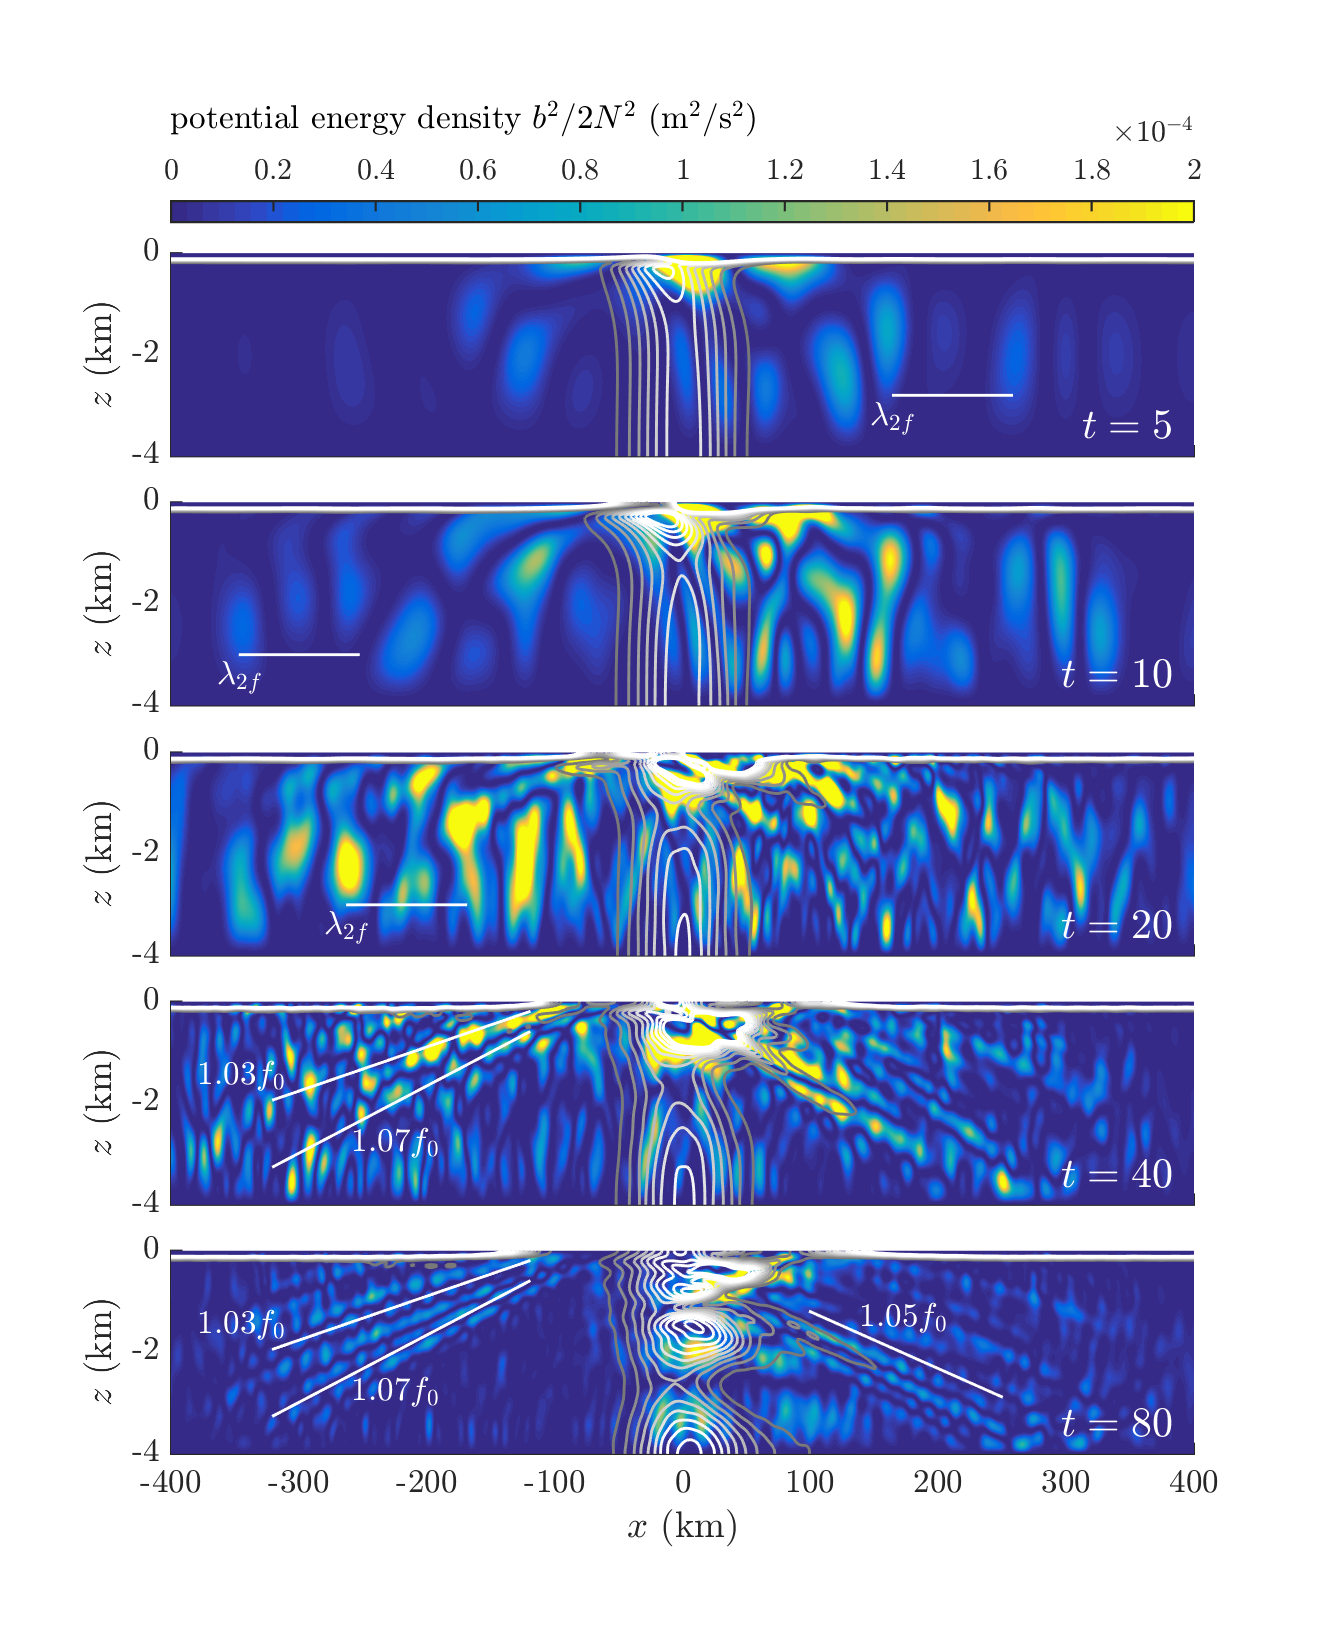
\includegraphics[height = 0.83\textheight]{introPdf}
\caption[The numerical solution to a two-dimensional Boussinesq initial value problem involving the interaction of a barotropic jet with a surface-concentrated near-inertial wave (NIW)]{The numerical solution to a two-dimensional Boussinesq initial value problem involving the interaction of a barotropic jet with a surface-concentrated near-inertial wave (NIW).  Shading shows potential energy density $b^2 / 2 N^2$ and contours show kinetic energy density at 10 levels between 0.01 and $0.1 \; \mathrm{m^2 \,  s^{-2}}$ at $t=5$ through $t=80$ inertial periods.  A horizontal line on the $t=5$, 10, and 20 snapshots shows the wavelength of a vertical mode-one $2f_0$-frequency internal wave.  The slanting lines on the $t=40$ and $t=80$ snapshots indicate the characteristic propagation angles of NIWs with the indicated frequencies.  The initial $v$ and $u$ are given in  \eqref{jet1} and \eqref{niw}, where $V_1 = 0.4 \, \mathrm{m \, s^{-1}}$, $L = 40 \, \mathrm{km}$, $U = 0.8 \; \mathrm{m \, s^{-1}}$, and $h=100 \; \mathrm{m}$.  Only the central 800km of a $1200$ km computational domain with 150 km thick sponge layers on either side is shown.}
\label{twof_intro}
\end{figure}

If the jet in \eqref{jet1} were not present, the initial condition in $u$ would develop into a perpetual, spatially uniform, non-propagating purely inertial wave.   Instead, refraction by the  imposed jet injects small horizontal scales of size $\sim \! \! L$ into the NIW field, induces near-inertial vertical propagation, and catalyzes radiation of low-mode $2f_0$ internal waves.  The development of this process is illustrated in figure \ref{twof_intro}, which shows snapshots of potential energy density at $t=5$, $10$, $20$, $40$, and $80$ inertial periods.  The kinetic energy density is indicated  by  10 overlain contours between 0.01 and 0.1 $\mathrm{m^2/s^2}$.  Throughout the simulation, kinetic energy remains localized in the surface layer and in the near-field of the barotropic jet; bulges in kinetic energy appearing at $t=20$ through $80$ inertial periods  reveal the progress of vertical NIW propagation and the modification of the balanced flow by the NIWs.  The kinetic-energy bulges are on the anti-cyclonic flank of the jet and show that NIW energy is refractively focused into the region of negative vorticity \citep{balmforth,LeeNiiler}. 

The vertical propagation of NIW kinetic energy is attended by an evolving potential energy field.  Its most conspicuous aspect is a signal that extends the full domain depth and radiates horizontally from the region of jet-NIW interaction.  In early stages, the potential energy signal has vertical mode-one structure.  A horizontal line on the panel at $t=20$ inertial periods indicates the horizontal wavelength of a mode-one, $2f_0$ frequency internal wave.  Remarkably, while this $2 f_0$ signal is generated by nonlinear NIW {\it self}-interaction in a small region, it rapidly radiates to fill a much larger volume without significant NIW activity (Danioux et al. 2008).

In addition to the low- and intermediate-mode $2f_0$ signal, narrow beams of potential energy radiate downwards and outwards from the center of the domain.  These beams are NIWs, which propagate at the characteristic angles indicated by slanting lines on the snapshots at $t=40$ and $t=80$ inertial periods.  These beams of near-inertial energy are produced by a scattering interaction between the surface-concentrated NIW and the jet.  The rightward radiating beams are NIWs escaping the region of negative jet vorticity. 

The two-dimensional NIW-jet interaction is thus characterized by at least three distinct phenomena: trapping of near-inertial energy in regions of negative balanced vorticity, beam-like radiation of near-inertial energy, and emission of $2f_0$ waves.  We use a multiple space- and time-scale expansion of the Boussinesq equations to construct a three-component model describing all of these processes.

\subsection{Summary of the three-component model}

In the three-component model, the horizontal velocity is 
\beq
u + \ii v \defn \ee^{-\ii f_0 t} \, \L A + \left ( - \p_y + \ii \p_x \right ) \psi + \cdots \per
\label{uvintro}
\eeq
where $A(x,y,z,t)$ is the NIW envelope and $\psi(x,y,z,t)$ is the quasi-geostrophic streamfunction.    The differential operator $\L$ in \eqref{uvintro} is defined below in \eqref{qwintro} and the $\cdots$ on the right of \eqref{uvintro} stand for additional contributions to horizontal velocity: NIW  harmonics, Stokes corrections, and ageostrophic flow.  The pressure field is 
\beq
p = f_0 \psi  + \frac{\ii f_0}{2} \Big [ \ee^{-\ii f_0 t} (\p_x - \ii \p_y ) A + \ee^{-2 \ii f_0 t} 2 B \Big ]  + \cc + \cdots \com
\label{pintro}
\eeq
where $B(x,y,z,t)$ is the $2f_0$ wave envelope, `$\cc$' stands for `complex conjugate', and the $\cdots$ indicate unimportant high-order corrections.  The vertical velocity $w$ is
\beq
w = - \frac{f_0^2}{2 N^2} \Big [ \ee^{-\ii f_0 t} (\p_x - \ii \p_y ) A_z + \ee^{-2 \ii f_0 t} 4 B_z \Big ] + \cc \per
\eeq
The $2f_0$ contribution in $B$ features prominently in the vertical velocity field, despite its small contribution to horizontal velocity.

The  system  consists of three equations: a wave-averaged quasi-geostrophic potential vorticity equation, the NIW equation, and a `$2f_0$ equation' governing the evolution of $2f_0$ waves.  The wave-averaged potential vorticity equation is
\beq
q_t + \sJ(\psi, q) = 0 \com 
\label{qintro}
\eeq
where the potential vorticity is
\beq
q = \Big(\underbrace{\mystrut{2ex} \p_x^2 + \p_y^2}_{\defn \hlap} + \underbrace{\mystrut{2ex} \p_z \frac{f_0^2}{N^2} \p_z}_{\defn \sL} \Big) \psi + \beta y +\frac{\ii}{2 f_0} \sJ \left ( \sL A^*, \sL A \right ) + \frac{1}{4 f_0} \hlap \bl \sL A \bl^2 \per
\label{qwintro}
\eeq
In \eqref{qintro} and \eqref{qwintro} the operator $\sJ(a,b)=a_x b_y - a_y b_x$ is the Jacobian, the inertial frequency is $f = f_0 + \beta y$, and $N(z)$ is the depth-dependent buoyancy frequency associated with strong background stratification.  The two rightmost terms in \eqref{qwintro} are quadratic NIW contributions to the wave-averaged potential vorticity.  Note that the $2f_0$ waves are assumed too weak to contribute appreciably to potential vorticity.  The evolution of the NIW field is described by a generalization of the YBJ equation,
\beq
 \L A_t + \tfrac{\ii}{2} f_0 \hlap A + \sJ(\psi, \L A) + \ii \hspace{0.2ex} \L A \big ( \half \hlap \psi + \beta y \big )  + \tfrac{1}{2} \L A^* \big ( \p_x + \ii \p_y \big )^{ \! 2} B = 0 \per
\label{niwintro}
\eeq
Equation \eqref{niwintro} accounts for NIW dispersion and group propagation, horizontal advection by balanced flows, refraction by balanced flows and non-uniform planetary vorticity, and nonlinear NIW-$2f_0$ interaction.  The NIW-$2f_0$ interaction term on the right end of \eqref{niwintro} is identical to the term introduced by Young, Tsang, and Balmforth (2008) \nocite{young2008near} into the YBJ equation to analyze near-inertial parametric subharmonic instability (PSI); in that work, the NIW-$2f_0$ interaction was implicated in the production of very small NIW vertical scales.  The evolution of the $2 f_0$ amplitude $B$ is obtained from 
\beq
\left ( \hlap + 13 \L \right ) B_t + 4 \ii f_0 \big ( \hlap - 3 \L \big ) B = - \tfrac{3}{2} \big ( \p_x - \ii \p_y \big )^2 \big ( \L A \big )^2 \per
\label{varpiintro}
\eeq
Equation \eqref{varpiintro} describes dispersion and group propagation of $2f_0$ waves, forced $2f_0$ oscillations, and energy transfer from NIWs into the $2f_0$ field.

The three-component model, comprised of equations \eqref{qintro} through \eqref{varpiintro}, describes the coupled evolution of near-inertial waves, quasi-geostrophic flow, and near-$2f_0$ internal waves.  Like the XV system, the three-component model conserves two integral quantities: `wave action', and `coupled energy'.  Wave action is a sum of NIW kinetic energy and the total energy of freely-propagating near-$2f_0$ waves.  Coupled energy is the sum of total balanced energy, near-inertial potential energy, a NIW-$\beta$ interaction term, and terms associated with the NIW-$2f_0$ interaction.  

A striking implication of both the XV and three-component model is that NIWs can extract energy from balanced flow.  This follows from the separation of wave action and coupled energy conservation, which requires that an increase in NIW potential energy during NIW-flow interaction comes at the expense of balanced energy.  Balanced flow thus loses energy when interacting with NIWs that consist almost entirely of kinetic energy, and NIW-QG interaction forms a link between large-scale balanced energy, the energy contained in the internal wave field, and wave breaking and diapycnal mixing.  XV refer to this wave-mean interaction as `stimulated loss-of-balance' to distinguish it from spontaneous loss-of-balance \citep{Vanneste2013}, emphasizing that it requires externally-forced waves to `stimulate' {\it further} production of wave energy at the expense of balanced energy.  Unlike spontaneous wave generation, stimulated wave generation is a potentially significant energy sink for nearly-balanced flows with small Rossby numbers. 

\bigskip \textit{The remaining main text and two appendices have been removed to reduce the file size of this dissertation template.}

\section{Near-inertial non-dimensionalization}
\section{The NIW equation} \label{niwexpansion}
\section{The NIW-averaged potential vorticity}
\section{Remodeling}
\section{Conservation laws} \label{conservationlaws}
\section{Comparison of three-component model and Boussinesq equations} \label{simulations}
\section{Energy transfer and production of small vertical scales}
\section{Discussion} \label{physicalImplications}

\begin{subappendices}

\section{A consistent two-dimensionalization of the three-component model}
\label{interruptedDecay}

The \tcm system in \eqref{qintro} through \eqref{varpiintro} reduces from three to two-dimensions when $N$ is constant, $\psi=\psi(x,y)$ is barotropic, and $A$ and $B$ are standing waves in the vertical such that
\beq
A(x,y,z,t) = \ee^{\ii mz} \phi(x,y,t) \com \qquad \text{and} \qquad B(x,y,z,t) = \ee^{2 \ii m z} \theta(x,y,t) \per
\label{standingWavesTwoDimensionalization}
\eeq
With the horizontal wavenumber
\beq
\kappa \defn m f_0 / N\com
\eeq
we find that 
\beq
\L A = - \ee^{\ii m z} \kappa^2 \phi \com \qquad \text{and} \qquad \L A^* = - \ee^{- \ii m z} \kappa^2 \phi^* \per
\eeq
Under the assumption that $\psi$ is barotropic and that $A$ and $B$ have standing wave structure with a single vertical wavelength, all $z$-dependent terms factor out of equations \eqref{qintro} through \eqref{varpiintro}, yielding a two-dimensional system without further approximation.  The two-dimensionality of $\psi$ and standing-wave structure of $A$ implies that $q$ is two-dimensional and still governed by horizontal advection so that
\beq
q_t + \J \left ( \psi, q \right ) = 0 \com \qquad \text{with} \qquad q = \hlap \psi + \beta y + \tfrac{\ii \kappa^4}{2 f_0} \sJ \left ( \phi^*, \phi \right ) + \tfrac{\kappa^4}{4 f_0} \hlap | \phi |^2 \com
\label{qTwoDim}
\eeq
The near-inertial equation \eqref{niwintro} reduces to
\beq
\phi_t  - \tfrac{\ii f_0}{2 \kappa^2} \hlap \phi  + \sJ \left ( \psi, \phi \right ) + \ii \phi \left ( \half \hlap \psi + \beta y \right ) + \half \phi^* \left ( \p_x + \ii \p_y \right )^2 \theta = 0 \per
\label{phiEqn}
\eeq
From \eqref{varpiintro} the two-dimensionalized $2f_0$ equation turns into
\beq
\left ( \hlap - 52 \kappa^2 \right ) \theta_t + 4 \ii f_0 \left ( \hlap + 12 \kappa^2 \right ) \theta = - \tfrac{3 \kappa^4}{2} \left( \p_x - \ii \p_y \right )^2 \phi^2 \per
\label{thetaEqn}
\eeq 
The two-dimensionalized \tcm system is equations \eqref{qTwoDim} through \eqref{thetaEqn}.  The model parameters are Coriolis frequency $f_0$ and its variation $\beta$, buoyancy frequency $N$, and near-inertial wavenumber $\kappa$.

The wave-wave interaction between near-inertial waves and the $2f_0$ harmonic is unimportant in the solutions of \eqref{qTwoDim} through \eqref{thetaEqn} reported here.  A possible reason is the similarity in vertical structure between $A$ and $B$, while the simulations in \ch \ref{introduction} indicate the significant interactions are between near-inertial and $2f_0$ waves of widely differing vertical scale.  Equivalently, with similar vertical wavenumbers for $A$ and $B$, resonant and near-resonant interactions are restricted to triads with widely differing \textit{horizontal} scale.  


\subsection{Scaling the strength of wave-induced mean flows}
\label{stimulatedScalingArguments}

The essential physics of \eqref{qTwoDim} and \eqref{phiEqn} are exposed by simple scaling arguments.  To fix ideas, consider the deposition of a uniform near-inertial velocity $-\kappa^2 \phi = \tilde U$ in a turbulent two-dimensional vorticity field $q$.  For now, we ignore the $2f_0$ field $\theta$.  The ensuing evolution clearly depends on the the wave magnitude $\tilde U$ and the spatial structure of $q$.  More obscure is the critical role played by the wave dispersivity, 
\beq
\hbar \defn \frac{f_0}{\kappa^2} = \frac{N^2}{m^2 f_0} \com
\eeq
which determines the strength of linear wave dispersion and controls the length-scales that develop dynamically in the near-inertial field.  This control over wave length-scales means that $\hbar$ determines the relative importance of wave field nonlinearity and magnitude of the wave-induced balanced flow.

The importance of dispersivity is revealed by examining the two dispersive balances possible in \eqref{phiEqn}, 
\beq
\hbar \hlap \phi \sim \J \left ( \psi, \phi \right ) \com \qquad \text{or} \qquad \hbar \hlap \phi \sim \phi \hlap \psi \per
\label{stimulatedBalances}
\eeq
The two balances in \eqref{stimulatedBalances} reflect a competition between the smoothing effects of dispersion and either stirring by advection or wave refraction.  If we neglect the wave-induced contribution to $\psi$ due to the $\phi$-dependent terms in \eqref{qTwoDim}, these balances imply two distinct scalings for $\tilde L$, the characteristic horizontal scale of $\phi$:
\beq
\text{advective: } \tilde L \sim \frac{\hbar}{\bar U}  \qquad \qquad \text{and} \qquad \qquad \text{refractive: } \tilde L \sim \sqrt{ \frac{\hbar \bar L}{\bar U}} \com
\label{stimulatedScalings}
\eeq
where $\bar L$ and $\bar U$ are characteristic length and velocity scales for $q$.  Since only dispersion can limit the reduction of $\tilde L$, the smaller of the two scalings determines $\tilde L$ and the dominant balance in \eqref{phiEqn}.  Thus for fixed $\bar U$ and ignoring the effect of wave nonlinearity, decreasing the scale of $| \grad \psi |\sim \bar U$ or increasing the dispsersivity $\hbar$ strengthens the refractive balance, while decreasing $\hbar$ leads to smaller scales in $\phi$ and strengthens the advective balance.  These scaling arguments, which ignore finite amplitude wave effects, were identified by \citet{danioux2015concentration} for a linearized shallow water near-inertial equation identical to \eqref{phiEqn} with $\psi$ prescribed.  \citet{danioux2015concentration} additionally identify the scaling $\tilde L \sim \bar L$ when advection and refraction are equally important.  

The scalings in \eqref{stimulatedScalings} make clear that the wave field nonlinearity measured by $\ep = \tilde U / f_0 \tilde L$ depends not only on the strength of the leading-order wave field through $\tilde U \sim \kappa^2 \phi$, but also on dispersivity through its control of $\tilde L$.  Dispersivity thus exerts an important influence on the ultimate magnitude of the nonlinear wave-induced mean flow and wave-turbulence coupled evolution.  To see this explicitly we use the decomposition $\psi = \psiq + \psiw$, where $\psiq$ is the streamfunction associated with APV through $\hlap \psiq = q$ and $\psiw$ is the wave-induced streamfunction defined through 
\beq
\hlap \psiw = - \tfrac{\ii \kappa^4}{2 f_0} \J \left ( \phi^* , \phi \right ) - \tfrac{\kappa^4}{4 f_0} \hlap | \phi |^2 \per
\label{waveInducedMeanFlow}
\eeq
From \eqref{waveInducedMeanFlow} we find the wave-induced flow magnitude $| \bnabla \psiw|$ scales with
\beq
| \bnabla \psiw | \sim \frac{\tilde U^2}{f_0 \tilde L} = \ep \, \tilde U \per%= \frac{f_0 \phi^2 \bar U}{\hbar^3} 
\label{meanFlowMagnitude}
\eeq
The wave-induced mean flow increases in magnitude when $\tilde L$ decreases, corresponding to the increasing distortion of the wave field and the increasing importance of wave nonlinearity.  When the advective balance from \eqref{stimulatedBalances} holds, the scaling in \eqref{meanFlowMagnitude} implies that in the weak dispersion regime, the magnitude of the wave-induced mean flow,
\beq
| \bnabla \psiw | \sim \frac{\tilde U^2 \bar U}{f_0 \hbar}
\eeq
is inversely proportional to the dispersivity.  The scaling analysis reveals how the initial magnitude of the near-inertial wave is not sufficient to predict $\ep$: the magnitude of the wave field nonlinearity measured by $\ep$ arises organically out of the wave-turbulence interaction and has an important dependence on wave dispersivity.

One caveat with the preceding scaling argument is its ignorance of the wave self-advection term $\J \left ( \psiw, \phi \right )$ that contributes to the advective balance in \eqref{stimulatedBalances}.  This advection term is an important piece of finite-amplitude wave evolution, and may act to arrest the decrease in $\tilde L$ with $\hbar$. 



\subsection{Near-inertial interruption of free turbulent decay}

We explore the dynamics in equations \eqref{qTwoDim} and \eqref{phiEqnImproved} with a brief exploration of the role of dispersivity in a physical scenario in which the free decay of two-dimensional turbulence from semi-random initial conditions is interrupted by the sudden deposition of a horizontally-uniform near-inertial wave.  We set both $\beta =0$ and $\theta \mapsto 0$ to focus solely on the wave-turbulence interaction.

In the preliminary stage, $q$ obeys the ordinary two-dimensional turbulence dynamics described by equation \eqref{qTwoDim} with $\phi=0$, and decays from the initial condition
\beq
\psi(x,y,0) = \psi_0 \Bigg ( \sum_{n=2}^{5} \left ( \tfrac{k_n}{k_2} \right )^{\! -1} \! \cos \left ( k_n x + X_{n} \right ) \Bigg ) \Bigg ( \sum_{n=2}^{5} \left (  \tfrac{k_n}{k_2}  \right )^{\! -1} \! \cos \left ( k_n y + Y_n \right ) \Bigg ) \com
\label{randomIC}
\eeq
where $k_n = 2 \pi n / L$ and the $X_n$ and $Y_n$ are random phases between 0 and $2 \pi$.  The magnitude $\psi_0$ is set so that $\Ro = \text{max} \left ( \hlap \psi \right ) / f_0 = 0.1$ initially.  With the initial condition in \eqref{randomIC}, $q$ is stretched and filamented rapidly at early times before eventually coalescing into a small number of roaming eddies over several hundreds of inertial periods.  The duration of the preliminary turbulent decay, $t_0$, thus determines the initial spatial structure of $q$.  In the results shown here the near-inertial wave is deposited after a relatively short preliminary integration of $t_0 = 200$ inertial periods corresponding roughly to $2 \pi t_0 / Ro \approx 120$ eddy turnover times.

We solve equations \eqref{qTwoDim} and \eqref{phiEqn} with pseudospectral method in a square and periodic domain in $x,y$ with $-L/2 < x,y < L/2$, $L = 400$ km and grid resolution $1024^2$ unless stated otherwise.  The buoyancy frequency is $N = 2 \times 10^{-3} \, \mathrm{s^{-1}}$ and the inertial frequency is $10^{-4} \, \mathrm{s^{-1}}$.  High order hyperdissipation is added for stability.  Some details of the pseudospectral method are described in \ch \ref{pseudospectralNumerics2D}.


An initial feel for the dynamics in \eqref{qTwoDim} and \eqref{phiEqn} is given by figure \ref{initialFeelEarly}, which compares vorticity evolution in ordinary decaying two-dimensional turbulence with vorticity evolution within a strong near-inertial wave field.  The vertical wavelength of the near-inertial wave is $2 \pi / m = 600$ m and its initial magnitude is around $\tilde U  = 0.2$ m/s so that $\ep / \Ro \approx \tilde U / \text{max} \left ( | \bnabla \psi | \right ) = 2$.  The advection associated with the near-inertial field gradually distorts the vorticity field away from the non-wave case.  The distortion ranges from fairly close correlation $t=50$ inertial periods the vorticity fields to the dramatic filamenting and distortion apparent at $t=400$ inertial periods.  The gradualness of the vorticity distortion corresponds to the relative weakness of the wave-induced balanced flow, which is roughly an order of magnitude weaker than the leading-order oscillation of the waves. 

A better understanding of the role of dispersivity is given by figure \ref{comparingTinySpectrums}, which compares snapshots of the vorticity field $q / f_0$, the wave-induced mean flow magnitude $| \bnabla \psi^{\mathrm{w}} |$, and the wave magnitude $\kappa^2 | \phi |$ after $t=400$ inertial periods of wave-turbulence coupled evolution for four values of $m$ and thus $\hbar$.  The initial state is the same used for figure \ref{initialFeelEarly} and consists of a uniform near-inertial wave with $\tilde U \approx 0.2$ m/s and vorticity field after $t_0 = 200$ inertial periods of initial decay from \eqref{randomIC}.  

\begin{sidewaysfigure}
\centering
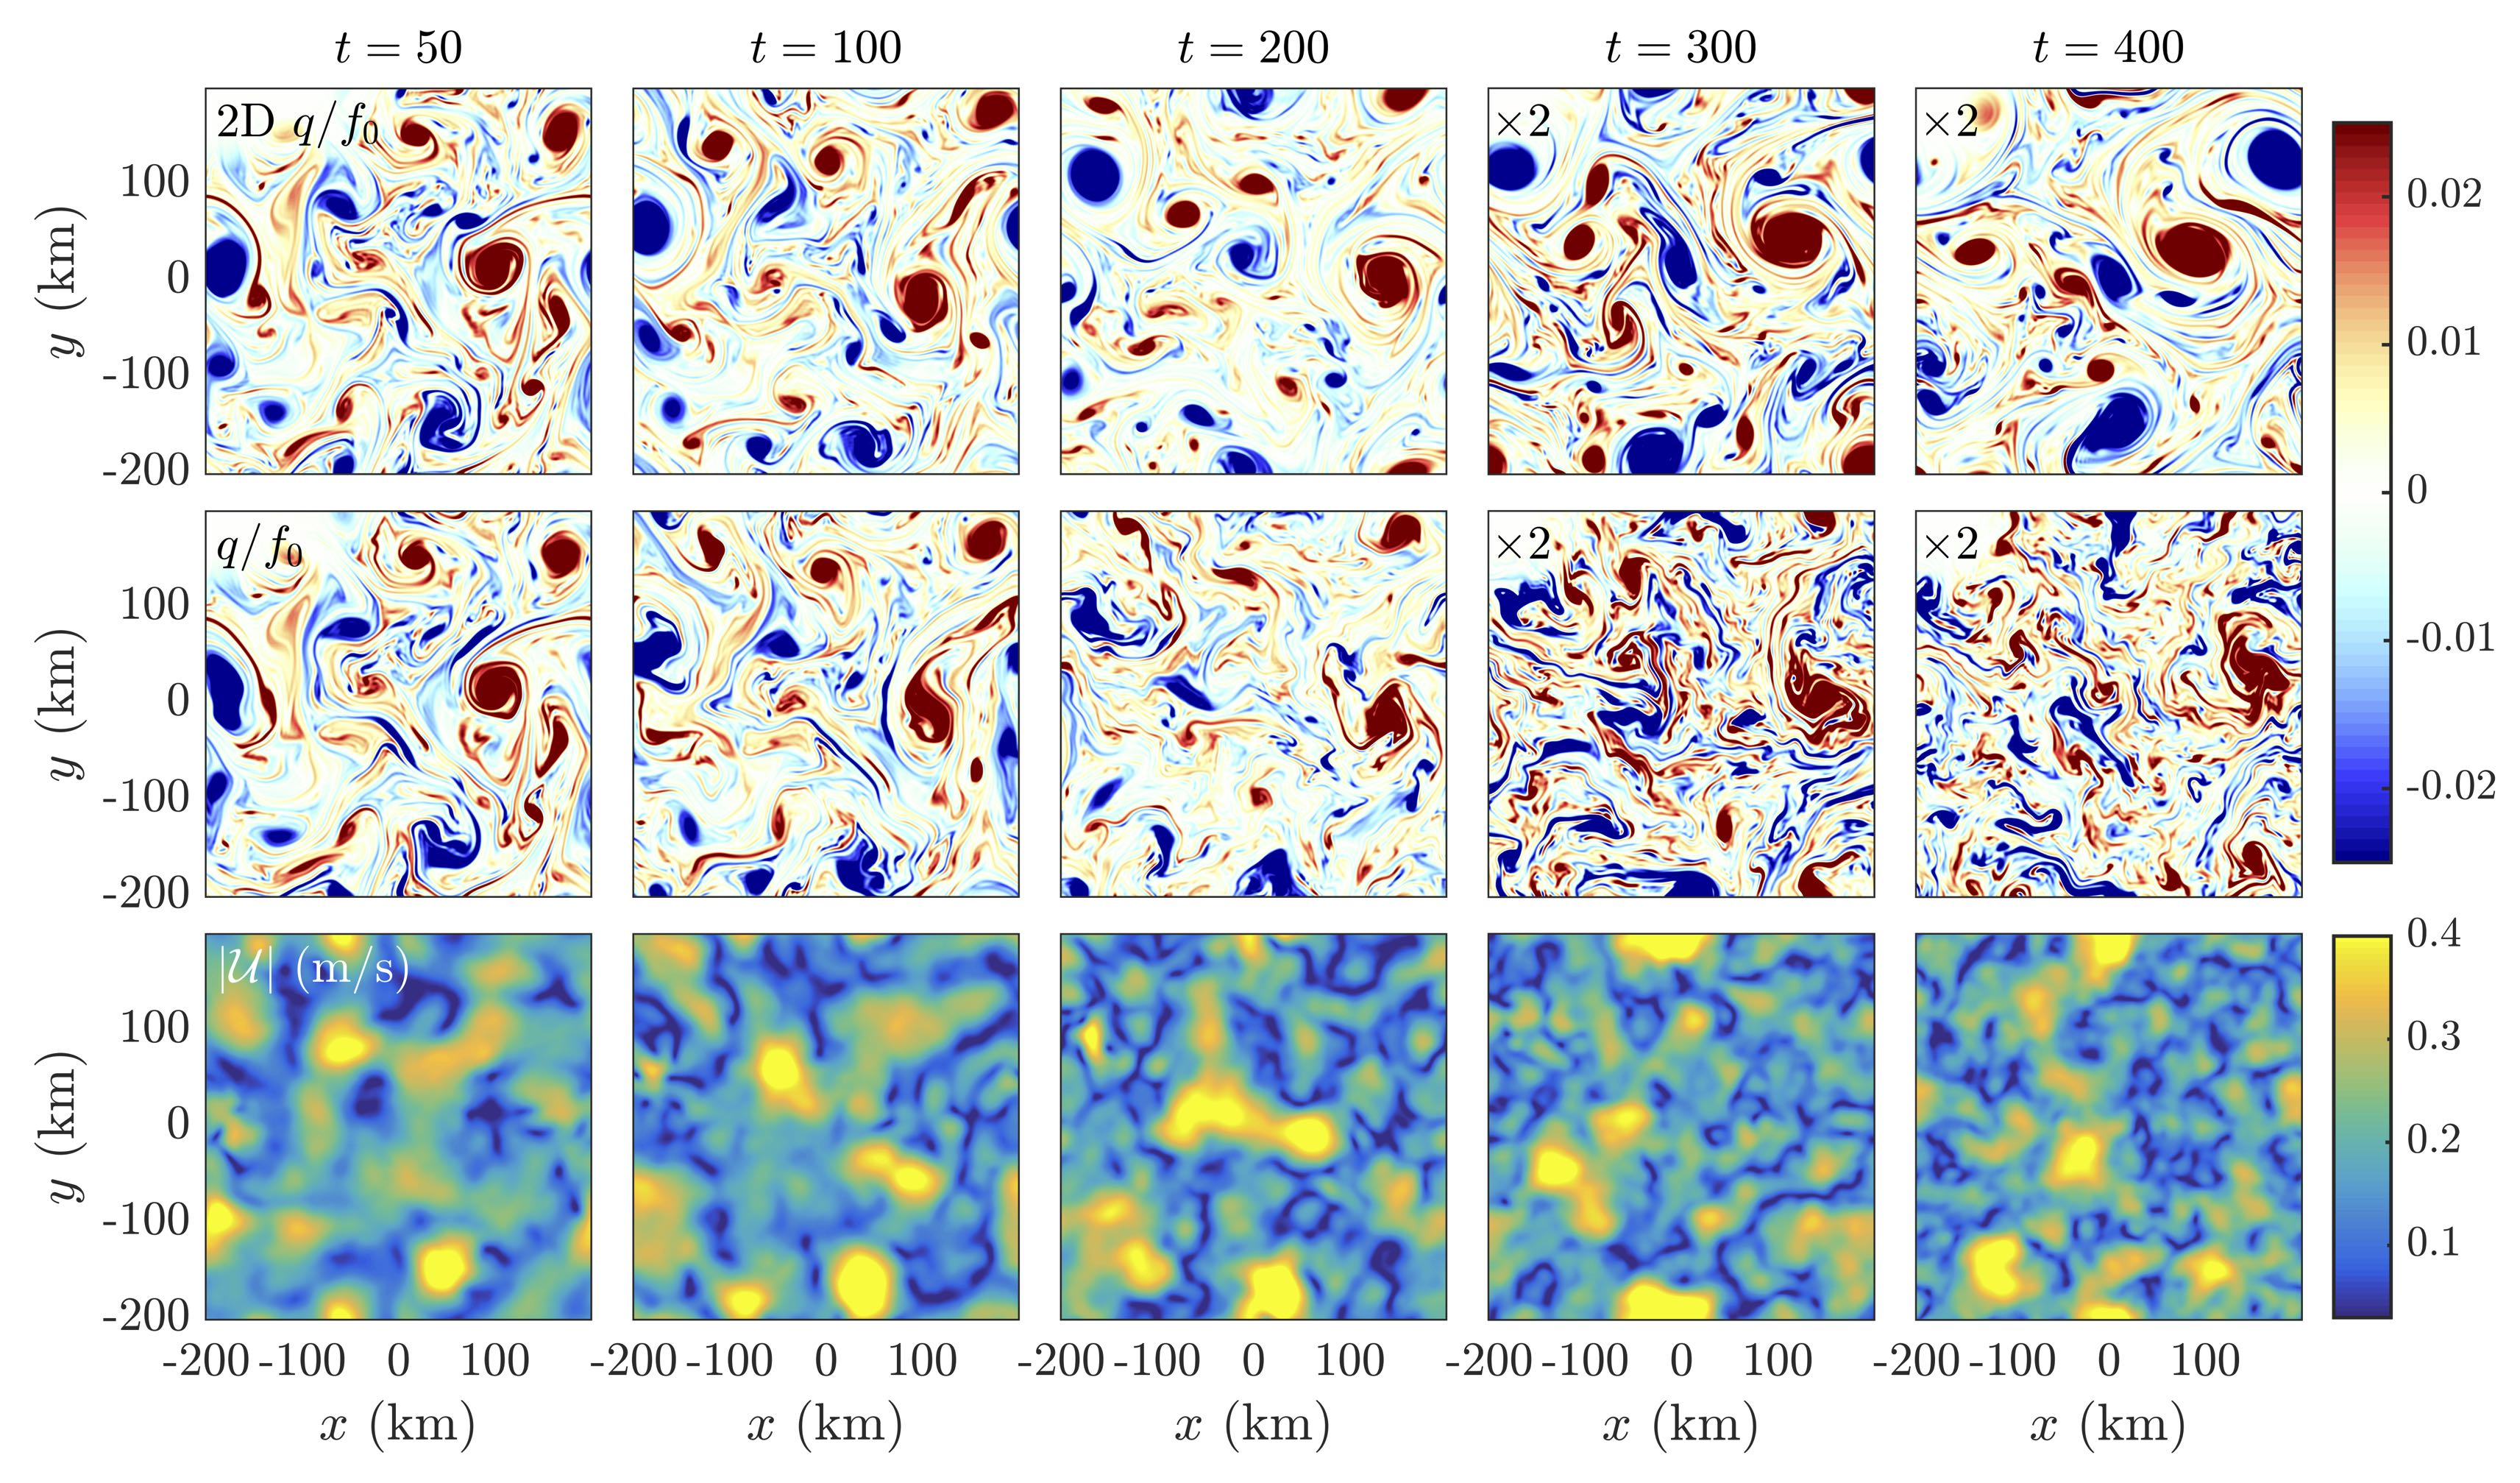
\includegraphics[width = 1\textwidth]{stimulatedEarlyEvolution}
\caption[Comparison of ordinary and wave-affected two-dimensional turbulent evolution]{Comparison of ordinary and wave-affected two-dimensional turbulent evolution.  The bottom two rows show the evolution of vorticity $q/f_0$ and near-inertial speed $\kappa | \phi |$ following the deposition of a uniform near-inertial wave with vertical wavelength $2 \pi / m = 600$ m into the vorticity field of decaying two-dimensional turbulence.  The top row shows the turbulent evolution of vorticity when waves are absent.  The turbulent vorticity field is generated by integrating \eqref{qTwoDim} with $\phi = 0$ for 200 inertial periods of preliminary turbulent decay.  Time increases from left to right from $t=50$ to $t=400$ inertial periods.  The flow has an initial maximum Rossby number of $\text{max}(q)/f_0 \approx 0.1$ and the initial wave-amplitude is chosen so that $\ep / \Ro \approx \tilde U / \text{max}(| \bnabla \psi |) = 2$.}
\label{initialFeelEarly}
\end{sidewaysfigure}

The dependence on wave dispersivity is clear: decreasing dispersivity leads to smaller and smaller scales in the wave velocity field $\kappa^2 | \phi |$.  The small-scales in $\phi$ lead in turn to a wave-induced mean flow $\bnabla \psiw$ which is both stronger and of smaller scale as dispersivity becomes weaker.  The increased strength and smaller scale of the vorticity-advecting flow $\bnabla \psiw$ means that wave fields with weaker dispersivity interact more strongly with the mean flow.  The effect of the waves becomes dramatic for the very small vertical wavelength $2 \pi / m = 200$ m on the far right, in which the smooth eddy structures of ordinary two-dimensional turbulence are replaced by a highly corrugated and filamentary vorticity field.  

The two-component, two-dimensional model in equations \eqref{qTwoDim} through \eqref{phiEqn} with $\theta \mapsto 0$ provides a convenient system to study the coupled evolution of mean vorticity and near-inertial waves.  The scaling argument in \ch \ref{stimulatedScalingArguments} reveals the crucial role of wave dispersivity or, alternatively, the vertical scale of the waves in setting the strength of the wave-turbulence interaction.  Waves with smaller vertical scales and thus weaker dispersion are more strongly distorted by turbulence, develop stronger wave-induced mean flows, exert more severe alterations on turbulent evolution, and extract more energy from the mean vorticity.  The qualitative nature of the scaling arguments is roughly confirmed by figure \ref{comparingTinySpectrums}, but both quantitative confirmation  and analysis of energy transfer between waves and flow awaits future work.  


\begin{figure}
\centering
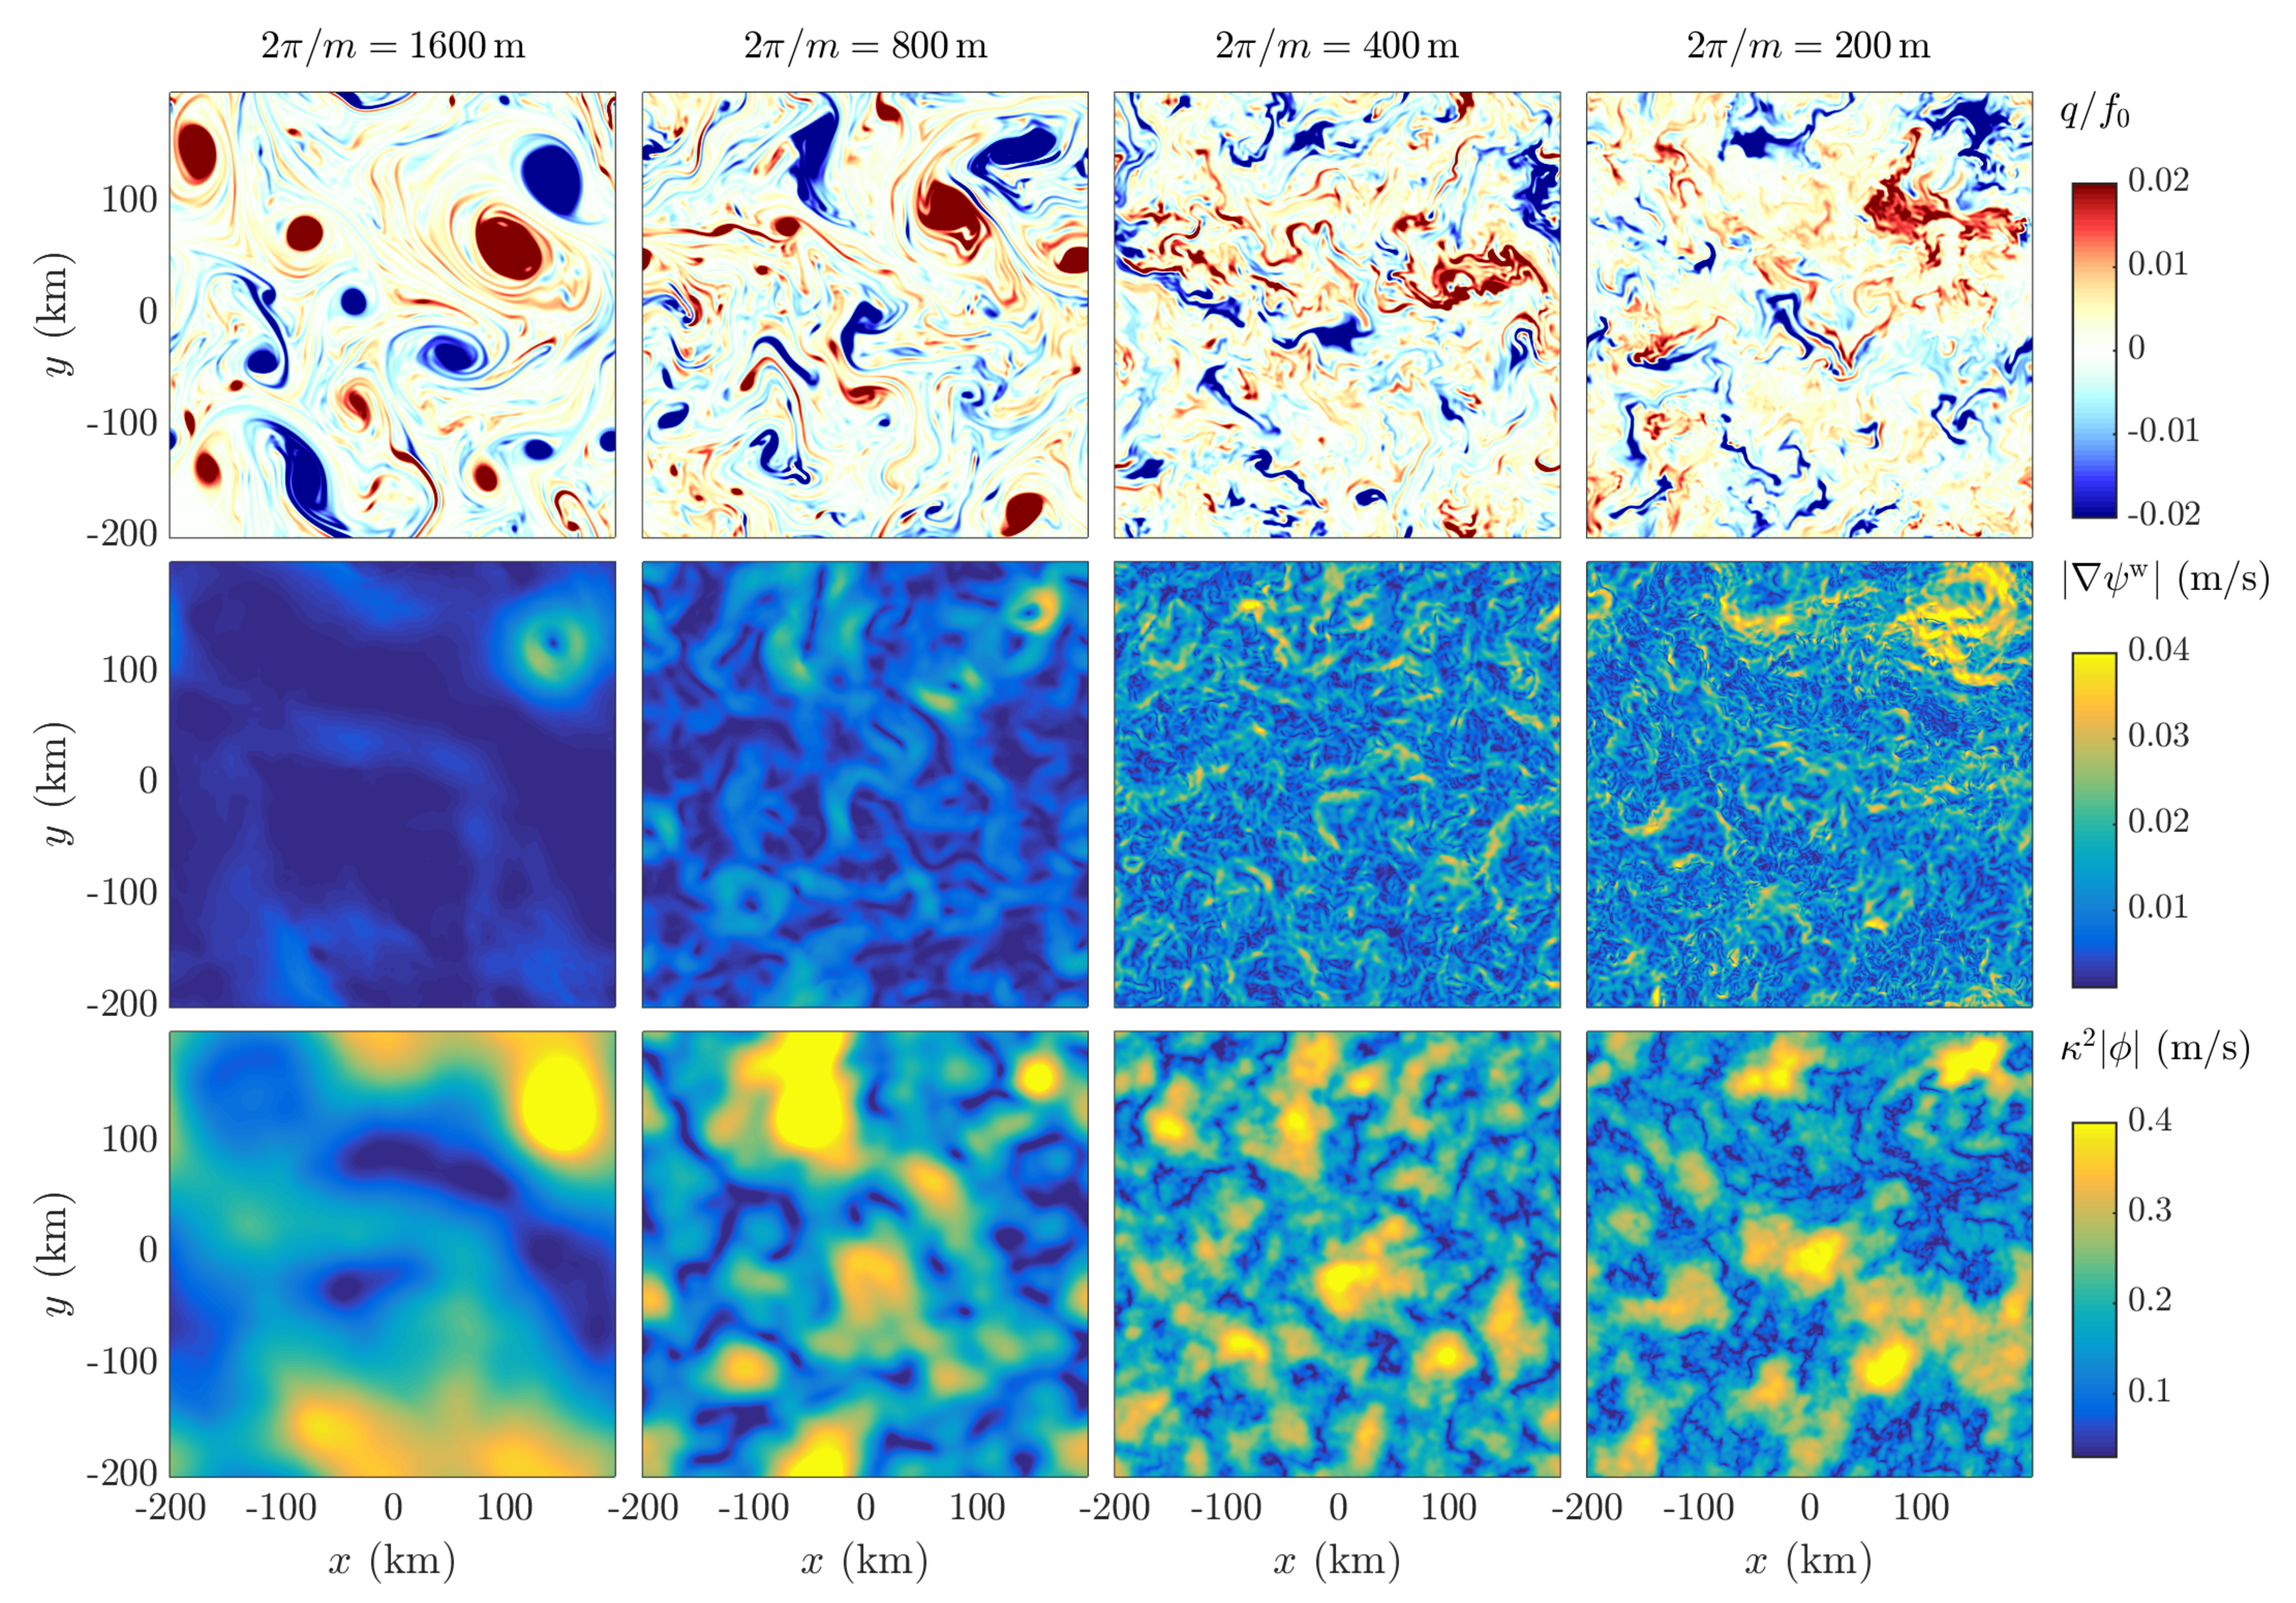
\includegraphics[width = 1\textwidth]{dispersivity_t400}
\caption[Effect of vertical wavenumber on coupled NIW and 2D turbulence evolution]{Effect of vertical wavenumber and thus wave dispersivity on the coupled evolution of NIWs and two-dimensional turbulence.  The four columns compare results for the four vertical wavelengths that label each column corresponding to the dispersivities $\hbar = 2594, 648.5, 162.1$, and $40.53 \; \mathrm{m^2/s}$.  The top row plots the vorticity $q/f_0$; the middle row plots the wave-induced mean flow speed $| \bnabla \psiw |$, and the bottom row plots the wave speed $\kappa^2 | \phi | = | \L A |$.  The initial vorticity and wave fields are the same as in figure \ref{initialFeelEarly} and all snapshots are taken from $t=400$ inertial periods.}
\label{comparingTinySpectrums}
\end{figure}

\subsection{The pseudospectral numerical method}
\label{pseudospectralNumerics2D}

Equations \eqref{qTwoDim} through \eqref{thetaEqn} can be solved on a periodic grid in $x,y$ with a pseudospectral numerical method.  For this we decompose $q$, $\phi$, and $\theta$ into Fourier modes, and denote their Fourier transforms with $\hat q$, $\hat \phi$, and $\hat \theta$.  $x$-wavenumbers are denoted by $k$ and $y$-wavenumbers by $\ell$, so that horizontal derivatives become
\beq
\phi_x \mapsto \ii k \hat \phi \qquad \text{and} \qquad \phi_y \mapsto \ii \ell \hat \phi \per
\eeq
We write the Jacobian $\J(a,b) = a_x b_y - a_y b_x$ and its transform as
\beq
\sJ \left ( a , b \right ) = \p_x \left ( a b_y \right ) - \p_y \left ( a b_x \right ) \com \quad \text{and} \quad \widehat{ \sJ (a,b) } = \ii k \, \widehat{ a b_y } - \ii \ell \, \widehat{ a b_x } \per
\eeq
Note that $\J(a,b) = \p_y \left ( a_x b \right ) - \p_x \left ( a_y b \right )$ and $\widehat{\J (a,b)} = \ii \ell \,\widehat{ a_x b} - \ii k \, \widehat{ a_y b }$ are also useful.  We also define 
\beq
q' \defn q - \beta y \quad \text{such that} \quad q' =  \hlap \psi + \tfrac{\ii \kappa^4}{2 f_0} \sJ \left ( \phi^*, \phi \right ) + \tfrac{\kappa^4}{4 f_0} \hlap | \phi |^2
\eeq
obeys
\beq
q'_t + \sJ(\psi,q') + \beta \psi_x = 0 \com \label{qp2d}
\eeq
The transform of \eqref{qp2d} is
\beq
\hat q_t + \D \hat q = - \widehat{ \sJ (\psi,q) } - \ii k \beta \, \hat \psi \com
\label{qp2dTransform}
\eeq
where $\D$ is a hyperdiffusion operator included for stability.  The transform of $q'$ 
%\beq
%\hat q = - K^2 \hat \psi - \tfrac{\kappa^4}{2 f_0} \Big [ k \, \widehat{\phi^* \phi_y} - \ell \, \widehat{ \phi^* \phi_x } \Big ]  - \tfrac{K^2 \kappa^4}{4 f_0} \widehat{ | \phi |^2 } \com
%\eeq
yields an inversion relation for $\hat \psi$,
\beq
\hat \psi = - \tfrac{1}{K^2} \hat q - \tfrac{\kappa^4}{2 K^2 f_0} \Big [ k \, \widehat{\phi^* \phi_y} - \ell \, \widehat{ \phi^* \phi_x } \Big ] - \tfrac{\kappa^4}{4 f_0} \widehat{ | \phi |^2 } \per
\eeq
The transform of the two-dimensionalized near-inertial equation \eqref{phiEqn} is 
\beq
\hat \phi_t + \tfrac{\ii f_0 K^2}{2 \kappa^2} \hat \phi + \D \hat \phi = - \widehat{ \sJ(\psi,\phi) } - \ii \reallywidehat{ \phi \left ( \half \hlap \psi + \beta y \right ) } - \half \widehat{ \phi^* \S \theta } \com
\label{phiEqnTransform}
\eeq
where $K^2 = k^2 + \ell^2$ and the operator $\S$ is 
\beq
\S \defn \left ( \p_x + \ii \p_y \right )^2 = \p_x^2 + 2 \ii \p_x \p_y - \p_y^2 \per
\eeq
Finally, equation \eqref{thetaEqn} transforms to
\beq
\hat \theta_t + \frac{ 4 \ii f_0 \left ( K^2 - 12 \kappa^2 \right )}{ K^2 + 52 \kappa^2} \hat \theta + \D \hat \theta = \frac{ 3 \left ( \ell^2 + 2 \ii k \ell - k^2 \right )}{ 2 \left ( K^2 + 52 \kappa^2 \right ) } \, \widehat{ \phi^2 }\per
\label{thetaEqnTransform}
\eeq
Notice that each of \eqref{qp2dTransform}, \eqref{phiEqnImprovedTransform}, and \eqref{thetaEqnTransform} take the form
\beq
\hat \phi_t + \mu_{\phi} \hat \phi = \cN_{\phi} \com
\eeq
where 
\begin{align}
\mu_q &= \D \com \\
\mu_{\phi} &= \frac{2 \ii f_0 K^2}{4 \kappa^2+ K^2} + \D \com \\
\mu_{\theta} &=  \frac{ 4 \ii f_0 \left ( K^2 - 12 \kappa^2 \right )}{ K^2 + 52 \kappa^2} + \D \per
\end{align}
$\D$ must be positive for it to damp the solution.  The $\cN$ are
\begin{align}
\cN_q &= \ii k \, \widehat{ \psi_y q } - \ii \ell \, \widehat{ \psi_x q } - \ii k \beta \, \hat \psi \com \\
\cN_{\phi} &= \ii k \, \widehat{ \psi_y \phi } - \ii \ell \, \widehat{ \psi_x \phi } - \ii \reallywidehat{ \phi \left ( \half \hlap \psi + \beta y \right ) } - \half \widehat{ \phi^* \S \theta } \com \\
\cN_{\theta} &= \frac{ 3 \left ( \ell^2 + 2 \ii k \ell - k^2 \right )}{ 2 \left ( K^2 + 52 \kappa^2 \right ) } \, \widehat{ \phi^2 } \per
\end{align}

\end{subappendices}

\section*{Acknowledgements}
\addcontentsline{toc}{section}{Acknowledgements}

Part of this chapter was submitted for publication in the \textit{Journal of Fluid Mechanics} by the author Gregory L. Wagner and William R. Young under the title `A three-component model for the coupled evolution of near-inertial waves, quasi-geostrophic flow, and the near-inertial second harmonic'.  The work was supported by the National Science Foundation under OCE-1357047.


% Chapter 4 ------------------------------------------------------------------- 
\let\cleardoublepage\relax \clearpage
\chapter{Slow evolution of internal tides in quasi-geostrophic flow}
\thispagestyle{preliminary}
\label{internalTideModelChapter}

\section{Introduction}

Internal tides are freely-propagating inertia-gravity waves with diurnal or semidiurnal tidal frequencies that are generated when surface tides slosh rotating and stratified water over rough bathymetry and underwater mountains.  The surface tides familiar to coastal life are essentially meter-high, depth-independent rotating shallow water waves forced by the gravitational pull of the sun and moon and predictable to within a centimeter in the open ocean.  \textit{Internal} tides have dynamically-unimportant surface displacements on the order of centimeters, depth-dependent interior density and velocity structure, and are much more difficult to predict because of their freely-propagating nature and modulation by quasi-geostrophic flows.  The name `internal tide' is potentially confusing because they are not directly forced by a harmonic gravitational perturbation.

Internal tides are an energetic and prominent component of motion almost everywhere in the Earth's ocean.  The ubiquity of their generation and basin-crossing propagation manifests in the striking global maps of their coherent mode-one surface signature extracted from decades of space-borne altimetry data by \citet{zhao2016global}.  And the role of internal tides in both ocean circulation and the astrodynamical evolution of the Earth and moon was demonstrated by \citet{egbert2000significant}, who constrained a shallow water surface tide model with long-term altimetry observations to show that roughly 25--30\% of the 3.75 terawatts dissipated from surface tides is converted to internal waves in the deep ocean.  Thus internal tides extract energy from the Earth-moon system, gradually slow the Earth's rotation, and contribute to the moon's outward drift of 3.82 cm per year.  At the same time, Egbert and Ray's result shows that internal tides are energetic enough to contribute to mixing processes that lift dense abyssal waters and thereby set the ocean's density stratification \citep{Ferrari2009}.  The detailed mechanisms and actual magnitude of the tidal contribution to abyssal mixing are yet unclear.

The ubiquity of internal tides also explains the irritation provoked by their contamination temporally-sparse observations intended to observe more slowly-evolving and persistent currents.  This aliasing issue confounds both ship-based hydrographic observations \citep{wunsch1975internal, munk1981internal} and planned altimetric observations of quasi-geostrophic flows with scales smaller than 50 km and faster than a month \citep{ponte2015incoherent}.

The scattering of oceanic internal tides by quasi-geostrophic flow is an important part of their dynamics over the long time-scales of their basin-crossing propagation and stymies the systematic removal of their contaminating signal from altimetric data.  In addition, the thought experiment by \citet{buhler2005wavecapture} and inferences from 1978-1979 POLYMODE Local Dynamics experiment data by \cite{polzin2010mesoscale} suggest that an energy budget for the ocean's quasi-geostrophic mesoscale should include a still-mysterious transfer of energy from quasi-geostrophic flows to the internal wave field.  Conceivably, quasi-geostrophic turbulence might lose energy or evolve with yet-undescribed dynamics when irradiated with a strong internal tide.  Finally, like the case of near-inertial waves described in \ch \ref{threeComponentModelChapter}, the distortion of internal tides by heterogeneous flows may precipitate nonlinear wave-wave interactions that transfer energy directly to the small spatial scales of wave breaking and mixing.  

%The need to understand internal tide propagation through quasi-geostrophic flows motivates \citet{rainville2006propagation}. 

%Put \citet{rainville2006propagation} and \citet{zaron2014time} in context.  And Kelly's papers?

We thus find two separate motivations to develop a slow evolution equation for the internal tide in quasi-geostrophic flow: \textit{(i)} to provide a potentially predictive model for internal tide propagation through quasi-geostrophic flow that is simpler than either the nonlinear or linearized Boussinesq equations; and \textit{(ii)} as the first step toward more sophisticated reduced models for the nonlinear coupled evolution and energetic interaction between internal tides, quasi-geostrophic flow, and possibly also near-inertial waves or tidal harmonics.  To this end, we assume the internal tide is a hydrostatic inertia-gravity wave, which limits our scope to mid-latitudes between roughly 15$^\circ$ and 60$^\circ$ latitude.  Poleward of 60$^\circ$, the tidal frequency becomes near-inertial and slow internal tide dynamics are better described by \cite{YBJ}'s near-inertial equation.  Equatorward of $15^\circ$, the vertical component of the Earth's rotation weakens to the point that both the horizontal component of Earth's rotation and non-hydrostatic dynamics are important for slow internal tide evolution.  

\subsection{Summary of the internal tide equation}

The principal result of this chapter is an equation that describes the slow evolution of internal tides in quasi-geostrophic flow.  In this slow internal tide equation, the pressure field is decomposed into a quasi-geostrophic and wave component, 
\beq
p = f_0 \left ( \psi + \ee^{- \ii \sigma t} A + \ee^{\ii \sigma t} A^* \right ) \com
\label{pressureIntro}
\eeq
where $\psi$ is the quasi-geostrophic streamfunction, $A$ is the complex amplitude of the wavy pressure field oscillating with frequency $\sigma$, and $f_0 = 4 \pi \sin \phi / \mathrm{day}$ is the constant local inertial frequency at latitude $\phi$.  Both $\psi$ and $A$ evolve slowly over time-scales much longer than $1/\sigma$.  The pressure in \eqref{pressureIntro} is a special solution justified only when initial conditions or oscillatory forcing projects onto a combination of motions with frequency $\sigma$ and nearly-balanced flow.  For the semidiurnal lunar tide $\sigma \approx 2 \pi / 12.421 \, \, \mathrm{hours^{-1}} \approx 1.4 \times 10^{-4} \, \mathrm{s^{-1}}$. 

The leading-order pressure in \eqref{pressureIntro} is related to hydrostatic buoyancy $b$ and velocity field $\bu = (u,v,w)$ through the linear hydrostatic Boussinesq equations, 
\beq
b = f_0 \left ( \psi_z + \ee^{-\ii \sigma t} A_z + \ee^{\ii \sigma t} A^*_z \right ) \com
\eeq
and
\beq
\bu = \pnabla \psi - \tfrac{1}{\alpha f_0} \left ( \ii \sigma \bnablad + f_0 \pnabla \right ) \ee^{-\ii \sigma t} A + \cc \com
\label{velocityIntro}
\eeq
where `cc' denotes the complex conjugate. Equation \eqref{velocityIntro} writes $\bu$ in terms of the two vector operators
\beq
\pnabla \defn - \p_y \bxh + \p_x \byh \qquad \text{and} \qquad \bnablad \defn \p_x \bxh + \p_y \byh - \frac{\alpha f_0^2}{N^2} \p_z \bzh \com
\label{operatorDefsIntro}
\eeq
which ultimately simplify the presentation.  

The derivation of the slow hydrostatic wave equation assumes that the nonlinear interaction of $\psi$ and $A$ induces small perturbations to a dominant linear balance in the hydrostatic Boussinesq equations \eqref{xmomAH} through \eqref{contAH}.  In that case, the form of $p$ in \eqref{pressureIntro} implies that $A$ approximately satisfies the linear dispersion constraint, 
\beq
0 \approx \Big ( \underbrace{\mystrut{2.2ex} \p_x^2 + \p_y^2}_{\defn \hlap} \, - \, \alpha \, \underbrace{\mystrut{2.2ex} \p_z \frac{f_0^2}{N^2} \p_z}_{\defn \L} \Big ) A = \disp A \com \qquad \text{where} \qquad \alpha \defn \frac{\sigma^2 - f_0^2}{f_0^2} \com
\label{dispersionConstraintIntro}
\eeq
and $N(z)$ is the buoyancy frequency reflecting a background density stratification with arbitrary vertical structure.  The operator 
\beq
\disp \defn \hlap - \alpha \L
\eeq
is the `dispersion operator' and $\alpha$ is an $O(1)$ frequency parameter.  The linear hydrostatic dispersion relation for constant $N$ implies $\alpha = \left ( N k / f_0 m \right )^2$ is the `wave Burger number' or squared aspect ratio for hydrostatic waves with horizontal wavenumber $k$ and vertical wavenumber $m$.  When $\alpha$ is small the wave is near-inertial and better described by the model in \ch \ref{threeComponentModelChapter}; when $\alpha$ is large non-hydrostatic effects become important.

The approximate equality $\approx$ in \eqref{dispersionConstraintIntro} would be exact if the wave field in $p$ were constrained to exactly satisfy the linear dispersion relation.  The essence of our derivation is relax the dispersion constraint by `reconstituting' the leading-order equation, $\disp A = 0$, with the first-order equation that describes the nonlinear interaction of $\psi$ and $A$.  The result is a slow evolution equation for $A$, 
\beq
\begin{split}
0 &= \big [ \hlap + \left ( 4 + 3 \alpha \right ) \L \big ] A_t + 2 \ii \sigma \disp A + \tfrac{2 \left ( 1 + \alpha \right)}{\alpha} \big [ \hlap \J \left ( \psi, A \right ) + \J \left ( \psi, \hlap A \right ) - \J \left ( \hlap \psi, A \right ) \big ] \\
& \qquad - \tfrac{2}{\alpha} \J \left ( \disp \psi, A \right )   + \tfrac{2 \ii \left ( 1+\alpha \right )^{1/2}}{\alpha} \Big [ 2 \J \left ( \psi_x, A_y \right ) - 2 \J \left ( \psi_y , A_x \right ) + \hnabla \bcdot \left ( \disp \psi \hnabla A \right ) \Big ] \\
& \qquad \qquad \qquad - 2 \ii \left ( 1+\alpha \right )^{1/2} \bnabla \bcdot \tfrac{f_0^2}{N^2} \left ( A_z \bnablad \psi_z + \psi_z \p_z \bnablad A \right ) \per
\label{internalTideEqnIntro}
\end{split}
\eeq
where the Jacobian operator is $\J(a,b) = a_x b_y - a_y b_x$.  Equation \eqref{internalTideEqnIntro} is a counterpart to the `YBJ' equation describing the slow evolution of near-inertial waves in three-dimensional quasi-geostrophic flow $\psi$ and arbitrary background stratification reflected in $N(z)$.  The greatly increased complexity of \eqref{internalTideEqnIntro} over the YBJ equation is the cost of considering more strongly dispersive hydrostatic waves with frequency $\sigma > f_0$. 

The reconstitution of the leading-order equation, $\disp A = 0$, with the first-order equation that contributes all the nonlinear terms in \eqref{internalTideEqnIntro} means that under weakly nonlinear conditions $\disp A$ is by far the largest contributor to \eqref{internalTideEqnIntro}.  Thus, as intimated in \eqref{dispersionConstraintIntro}, the pressure field $p$ corresponding to solutions of \eqref{internalTideEqnIntro} \textit{almost} satisfies the linear dispersion relation for hydrostatic internal waves with frequency $\sigma$.  \citet{roberts1985introduction} explains how the method of reconstitution permits equations like  \eqref{internalTideEqnIntro} or the Navier-Stokes equation to describe a broader range of dynamics than would be permitted by more ceremonious asymptotic expansions.  The benefit of reconstitution to \eqref{internalTideEqnIntro} is a description of the slow evolution of more spatial modes of $A$ than would be allowed if the solution were restricted to those that exactly satisfy $\disp A = 0$ and thus the exact hydrostatic dispersion relation. 

%We begin our derivation by non-dimensionalizing the hydrostatic Boussinesq equations and their associated `wave operator form' in \ch \ref{equationsTide}.  In \ch \ref{waveEquationDerivationTide} we derive and make finishing touches to the model.  In \ch \ref{quasigeostrophicEvolutionTide} we establish that $\psi$ obeys quasi-geostrophic dynamics and in \ch \ref{examplesTide} we present some example solutions for hydrostatic wave propagation in barotropic flows that illustrate the power and limitations of equation \eqref{internalTideEqnIntro}.  We wrap up and contemplate future hopes for the slow wave equation and its relatives in \ch \ref{discussionTide}.

\section{Hydrostatic internal waves in barotropic flow} \label{examplesTide}

% ----------------------------------------------------------------------------- 
% Appendices
% ----------------------------------------------------------------------------- 
\appendix

\clearpage
\newcommand{\bOmega}{\boldsymbol{\Omega}}
\chapter{The Boussinesq equations and `wave operator form'}
\label{waveOperatorFormAppendix}

Writing the Boussinesq equations in different ways illuminates important aspects of Boussinesq physics.  Particularly useful in this dissertation is the `wave operator form', in which terms are rearranged until a linear wave operator is obtained acting on either $w$ in the non-hydrostatic equations, or $p$ in the hydrostatic equations.  In this view the nonlinear parts of the resulting equation can be viewed either as a source of waves in the case of spontaneous generation, or as the agent of weakly nonlinear evolution for the leading-order linear solution.  We begin the appendix by writing down the Boussinesq equations in an Earth-relevant rotating frame.

In a frame that rotates with angular velocity $\bOmega$ with the components
\beq
2 \bOmega = \underbrace{ \mystrut{1ex} 2 \Omega \sin \phi }_{\defn f_v} \bzh + \underbrace{ \mystrut{1ex}2 \Omega \cos \phi}_{\defn f_h} \byh \com
\eeq
the Boussinesq equations become
\begin{align}
\Dt{u} - f_v v + f_h w + p_x &= 0 \com \label{xmomFull} \\
\Dt{v} + f_v u + p_y &= 0 \com \label{ymomFull} \\
\Dt{w} - b + f_h u + p_z &= 0 \com \label{zmomFull} \\
\Dt{b} + w N^2 &= 0 \com \label{buoyFull} \\
u_x + v_y + w_z &= 0 \per \label{contFull}
\end{align}
At midlatitudes $f_v \sim f_h$.  For motions with horizontal scale $L$ and vertical scale $H$, the vertical velocity is small and scales with $w \sim \tfrac{H}{L} u$.  For motions with time-scales $f_v \sim f_h$, this means that $w_t / f_h u \sim H/L$ is small, and that $w_t$ and $f_h u$ can only be consistently neglected at the same time when the hydrostatic balance $p_z \sim b$ dominates the vertical momentum equation.  

\section{In the non-hydrostatic Boussinesq equations}
\label{nonhydrostaticDerivationA}

With $f_h = 0$, $f_v = f_0$ constant and expanding $\Dt{} = \p_t + \bu \bcdot \bnabla$, the Boussinesq equations in \eqref{xmom} through \eqref{cont} become
\begin{align}
u_t - f_0 v + p_x &= - \bu \bcdot \bnabla u \com \label{xmomA} \\
v_t + f_0 u + p_y &= - \bu \bcdot \bnabla v \com \label{ymomA} \\
w_t - b  + p_z &= - \bu \bcdot \bnabla w \com \label{zmomA} \\
b_t + w N^2 &= - \bu \bcdot \bnabla b \com \label{buoyA} \\
u_x + v_y + w_z &= 0 \per \label{contA}
\end{align}
We note that the assumption $f_h = 0$ while retaining $\Dt{w}$ in the vertical momentum equation \eqref{zmomA} is not really consistent for the long-time evolution of waves except perhaps at polar latitudes. 

To arrive at the wave operator form we first form three intermediate equations: the `oscillation equation', the `divergence equation', and the `vertical vorticity' equation.  The oscillation equations follows by adding $\p_t$\eqref{zmomA} to \eqref{buoyA}, 
\beq
w_{tt} + w N^2 + p_{zt} = - \Big [ \p_t \left ( \bu \bcdot \bnabla w \right ) + \bu \bcdot \bnabla b \Big ] \per
\label{oscEqnA}
\eeq
The divergence equation follows from adding $\p_x$\eqref{xmomA} to $\p_y$\eqref{ymomA} and using $u_x + v_y = -w_z$, 
\beq
w_{zt} + f_0 \omega - \hlap p = \p_x \left ( \bu \bcdot \bnabla u \right ) + \p_y \left ( \bu \bcdot \bnabla v \right ) \com
\label{divEqnA}
\eeq
where $\omega \defn v_x - u_y$ is the vertical component of vorticity, $\bomega = \bnabla \times \bu$, and $\hlap \defn \p_x^2 + \p_y^2$ is the horizontal Laplacian.  The vertical vorticity equation is formed by subtracting $\p_y$\eqref{xmomA} from $\p_x$\eqref{ymomA},
\beq
\omega_t - f_0 w_z = - \p_x \left ( \bu \bcdot \bnabla v \right ) + \p_y \left ( \bu \bcdot \bnabla u \right ) \per
\label{vorEqnA}
\eeq
Two more steps yield the wave operator form.  First, $f_0 \p_z$\eqref{vorEqnA} subtracted from $\p_z \p_t$\eqref{divEqnA} yields
\beq
\left ( \p_t^2 + f_0^2 \right ) w_{zz} - \hlap p_{zt} = \p_z \left ( \p_x \p_t + f_0 \p_y \right ) \left ( \bu \bcdot \bnabla u \right ) + \p_z \left ( \p_y \p_t - f_0 \p_x \right ) \left ( \bu \bcdot \bnabla v \right ) \per 
\eeq
Adding this to $\hlap$\eqref{oscEqnA} then gives
\beq 
\Big [ \p_t^2 \left ( \hlap + \p_z^2 \right ) + f_0^2 \p_z^2 + N^2 \hlap \Big ] w = \p_z \left ( \p_t \bnabla + f_0 \pnabla \right ) \bcdot \left ( \bu \bcdot \bnabla \right ) \bu - \hlap \left ( \bu \bcdot \bnabla b \right ) \com
\label{waveOperatorFormA}
\eeq
where $\pnabla \defn -\p_y \bxh + \p_x \byh$.  Equation \eqref{waveOperatorFormA} is the Boussinesq formulation that we call `wave operator form'.  

%\textcolor{red}{Indicial notation and comment about Lighthill theory.}

\section{In the hydrostatic Boussinesq equations}

The hydrostatic Boussinesq equations are a simplification of equations \eqref{xmomA} through \eqref{contA} justified when vertical accelerations are small compared to buoyancy forces.  The smallness of $\Dt{w}$ permits the reduction of \eqref{zmomA} to
\beq
p_z = b \com
\eeq
or hydrostatic balance.  Equations \eqref{xmomA} through \eqref{contA} then become
\begin{align}
u_t - f_0 v + p_x &= - \bu \bcdot \bnabla u \com \label{xmomAH} \\
v_t + f_0 u + p_y &= - \bu \bcdot \bnabla v \com \label{ymomAH} \\
p_z &= b \com \label{zmomAH} \\
b_t + w N^2 &= - \bu \bcdot \bnabla b \com \label{buoyAH} \\
u_x + v_y + w_z &= 0 \per \label{contAH}
\end{align}
The hydrostatic version of \eqref{waveOperatorFormA} is obtained by repeating the derivation in \ch  \ref{nonhydrostaticDerivationA} with $w_t$ and $\bu \bcdot \bnabla w$ set to zero,
\beq
\Big [ \left ( \p_t^2 + f_0^2 \right ) \p_z^2 + N^2 \hlap \Big ] w = \p_z \left ( \p_t \hnabla + f_0 \pnabla \right ) \bcdot \left ( \bu \bcdot \bnabla \right ) \bu - \hlap \left ( \bu \bcdot \bnabla b \right ) \com
\eeq
where 
\beq
\hnabla \defn \p_x \bxh + \p_y \byh
\label{horizontalNabla}
\eeq
has the horizontal components of $\bnabla$. 

\subsection{An alternative hydrostatic wave operator form}

Equations \eqref{xmomAH} through \eqref{contAH} have an alternative wave operator formulation which is expressed in terms of pressure $p$ rather than vertical velocity $w$.  To obtain this we first add $\p_t$\eqref{zmomAH} to $\p_z N^{-2}$\eqref{buoyAH} and use \eqref{contAH} to find
\begin{align}
u_x + v_y &= - w_z \com \\
&= f_0^{-2} \L p_t + \p_z \frac{1}{N^2} \left ( \bu \bcdot \bnabla p_z \right ) \per
\label{alternateContinuity}
\end{align}
Subtracting $\p_y$\eqref{xmomAH} from $\p_x$\eqref{ymomAH} and using \eqref{alternateContinuity} and multiplying the result by $f_0^3$ yields the vertical vorticity equation, 
\beq
f_0^3 \omega_t +  f_0^2 \L p_t = - f_0^3 \p_x \left ( \bu \bcdot \bnabla v \right ) + f_0^3 \p_y \left ( \bu \bcdot \bnabla u \right ) - f_0^2 \p_z \frac{f_0^2}{N^2} \left ( \bu \bcdot \bnabla p_z \right ) \per
\label{hydrostaticVerticalVorticity}
\eeq
Next, adding $\p_x$\eqref{xmomAH} to $\p_y$\eqref{ymomAH} using \eqref{alternateContinuity} and operating on the result with $ f_0^2 \p_t$ leads to
\beq
\p_t \big ( \p_t^2 \L + f_0^2 \hlap \big ) p + \p_z \p_t^2 \frac{f_0^2}{N^2} \left ( \bu \bcdot \bnabla p_z \right ) - f_0^3 \omega_t = - f_0^2 \p_t \p_x \left ( \bu \bcdot \bnabla u \right ) - f_0^2 \p_t \p_y \left ( \bu \bcdot \bnabla v \right ) \per
\label{hydrostaticDivergence}
\eeq
Adding \eqref{hydrostaticDivergence} to \eqref{hydrostaticVerticalVorticity} eliminates $f_0^3 \omega_t$ and thus produces the wave operator form of \eqref{xmomAH} through \eqref{contAH},
\beq
\p_t \Big [ \p_t^2 \L + f_0^2 \left ( \hlap + \L \right ) \Big ] p = - f_0^2 \left ( \p_t \hnabla + f_0 \pnabla \right ) \bcdot \left ( \bu \bcdot \bnabla \right ) \bu - \p_z \frac{f_0^2}{N^2} \left ( \p_t^2 + f_0^2 \right ) \left ( \bu \bcdot \bnabla p_z \right ) \com
\label{hydrostaticWaveOperatorFormA}
\eeq
where $\hnabla$ is the horizontal gradient defined in \eqref{horizontalNabla}.  The definition of the vector operator
\beq
\Sv \defn \p_t \hnabla + f_0 \pnabla 
\eeq
offers slight convenience for expressing \eqref{hydrostaticWaveOperatorFormA}.

% ----------------------------------------------------------------------------- 
% Bibliography
% ----------------------------------------------------------------------------- 
\clearpage
\singlespacing
\bibliographystyle{jfm}
\bibliography{refs}
\addcontentsline{toc}{chapter}{Bibliography}

\end{document}
